%%%%% META DATA %%%%%%%%%%%%
\newcommand\Course{Algebra for Secondary Mathematics Teaching} % e.g., Algebra, Geometry, Modeling, Statistics
\newcommand\Location{MODULE($\textnormal{S}^2$)} % affiliation and course
\newcommand\Term{Spring 2018} % term taught

 \newcommand\MODULES{$\textnormal{MODULE}(\textnormal{S}^2)$}
 \title{{\normalsize{Mathematics Of Doing, Understand, Learning, and Educating Secondary Schools} }\\  $\;$ \\ \MODULES: \\  \Course}
 \author{Adapted for \Location} 
 \date{Version \Term} 
 
 % Input a course graphic or leave the { } empty:
\newcommand\coursegraphic{DoubleRectangles.png} 
 
 %%%%%%%DOCUMENT FORMATTING %%%%%%%%%%
\documentclass[11pt]{article}
\linespread{1.03}% 6 lpi http://tex.stackexchange.com/questions/23824/6-lines-in-one-inch
\parskip6pt
\usepackage{amsmath, amsthm, amsfonts, amssymb, mathpazo, url, graphicx, stackrel, mdwlist, enumitem, mdframed, ifthen}
	% usual suspects, palatino, hyperlink capability, PDF graphics, symbol stacking, list customizations, boxes, ifthenelse macros
\usepackage[top=1in,bottom=1in,left=1in,right=1in]{geometry} % 8.5" x 11" pages with 1 inch margins
\usepackage[pdftex, bookmarks, colorlinks, breaklinks]{hyperref} % prettier hyperlinks
\usepackage[usenames,dvipsnames,svgnames,table]{xcolor} % defines colors for text and tikz graphics
\definecolor{darkred}{rgb}{0.8,0.1,0.2} % for hyperlinks
\definecolor{darkblue}{rgb}{0.2,0.1,0.7} % for hyperlinks
\hypersetup{linkcolor=darkred,citecolor=blue,filecolor=dullmagenta,urlcolor=darkblue} % colors for links
\usepackage[none]{hyphenat} % prettier hyphenating
\raggedright \parskip4pt  \parindent0pt 
\usepackage{array} % tables with paragraphs of set widths
\renewcommand{\arraystretch}{1.3} % makes tables more legible
\newcolumntype{L}[1]{>{\raggedright\let\newline\\\arraybackslash\hspace{0pt}}p{#1}}
\newcolumntype{C}[1]{>{\centering\let\newline\\\arraybackslash\hspace{0pt}}p{#1}}
\newcolumntype{R}[1]{>{\raggedleft\let\newline\\\arraybackslash\hspace{0pt}}p{#1}}
\usepackage{rotating} % rotating figures and tables, provides sidewaystable and sidewaysfigure
\usepackage{lipsum} % text testing


%%%%%%% DOCUMENT MANAGEMENT %%%%%%%%%%%%
% To do notes and commenting 
\usepackage{comment}

% View instructor notes 
\newif\ifinstructor 
\instructortrue  % view as instructor 
% \instructorfalse  % view as student
  
%%%%%%% SECTION FORMATTING %%%%%%%%%%%%
% sections
\usepackage{titlesec}
\titleformat{\subsection}[block]{\Large \bfseries \filcenter}{}{0em}{}
\titleformat{\subsubsection}[block]{\large \scshape\filcenter}{}{0em}{}
\newcommand{\handout}{\subsubsection}
\newcommand\header[1]{\vspace*{4pt}\par {\large {\bf #1}}\par}
\newcommand\about{\textasciitilde}

% itemize - second layer is an open circle instead of dash
\def\labelitemii{$\circ$}

% table colors - mostly for fun
\definecolor{yellow}{RGB}{255, 255, 0}
\definecolor{red}{RGB}{226, 30, 60}
\definecolor{orange}{RGB}{255, 159, 12}
\definecolor{green}{RGB}{16, 168, 112}
\definecolor{blue}{RGB}{1,200,255}
\definecolor{periwinkle}{RGB}{200,200,255}
\definecolor{lightteal}{RGB}{200,250,250}
\definecolor{purple}{RGB}{113, 1, 232}
%\definecolor{pink}{RGB}{255,70,192}
\definecolor{pink}{RGB}{232,1,193}
\definecolor{gray}{RGB}{100, 100, 100}

% instructor notes
\ifinstructor 
\newenvironment{bignote}[1][Instructor note]% default note is an "Instructor Note"
	{\begin{mdframed}\raggedright{\bf #1.~}}
	{\end{mdframed}}  
\else \excludecomment{bignote}
\fi

\ifinstructor
\newcommand\smallnote[1]
	{\begin{mdframed}\raggedright  {\bf Instructor note.} {#1} \end{mdframed}}
\else \newcommand\smallnote[1]{}
\fi

\ifinstructor  \usepackage{todonotes} 
\else \usepackage[disable]{todonotes}
\fi

% in-class task
\newenvironment{task}
	{\begin{mdframed}[linecolor=lightgray, linewidth=3pt]\raggedright}
	{\end{mdframed}}

%%% GRAPHICS / TIKZ %%%%%%%%%%%
\graphicspath{{Images/}}

\usepackage{tikz}
\usepackage{tkz-euclide} % tikz package for Euclidean geometry
\usepackage{siunitx} % typesetting quantities
\usepackage{pgfplots} %\pgfplotsset{compat=1.13} % plotting graphs
\usetikzlibrary{calc} % calculations within tikz
\usetkzobj{all} % needed for tkz-euclide package
 
%%%%% MATH NOTATION %%%%%%%%

\newcommand\tn{\textnormal}

% systems
\newcommand{\R}{\mathbb{R}}
\newcommand{\C}{\mathbb{C}}
\newcommand{\Q}{\mathbb{Q}}
\newcommand{\N}{\mathbb{N}}
\newcommand{\Z}{\mathbb{Z}}

% notation tweaking
\renewcommand\phi\varphi  % normal \phi looks too much like the empty set.
\renewcommand\subset\subseteq 
\renewcommand\supset\supseteq  % to be careful about strict subsets and nonstrict subsets
\newcommand\st{:}

% divisibility
\newcommand\divides{\;|\;}
\newcommand\notdivides{\hspace*{-2pt}\not |\;}

% trig and geometry
\newcommand\degrees{^\circ}

%%%%%%%%%% THEOREMS AND RELATED STRUCTURES %%%%%
\renewcommand\emph[1]{\underline{\bf{#1}}} % terminology

\newtheorem{theorem}{Theorem}[section]
\newtheorem{proposition}[theorem]{Proposition}
\newtheorem{lemma}[theorem]{Lemma}
\newtheorem{corollary}[theorem]{Corollary}
\newtheorem{claim}{Claim}

\theoremstyle{definition}
\newtheorem{definition}[theorem]{Definition}
\newtheorem{example}[theorem]{Example}
\newtheorem{problem}[theorem]{Problem}
\newtheorem{conjecture}[theorem]{Conjecture}
\newtheorem{question}[theorem]{Question}
\newtheorem{remark}[theorem]{Remark}
\newtheorem{case}{Case}

\newtheorem*{theorem*}{Theorem}
\newtheorem*{example*}{Example}
\newtheorem*{question*}{Question}
\newtheorem*{claim*}{Claim}
\newtheorem*{definition*}{Definition}

\newenvironment{solution}{{\it Solution.} }{\hfill {\color{lightgray}$\blacksquare$}}

\newcommand\qedpart[1]{ \hfill \framebox(6,6){\tiny #1}}
\renewcommand\qed{\hfill \framebox(6,6){}}
%%%%%%%%%%%%%%%%%%%%%%%%%%%%%%%% 	
%%%%%%%% DOCUMENT BEGINS %%%%%%%%%%%%
%%%%%%%%%%%%%%%%%%%%%%%%%%%%%%%% 

\begin{document}

%%%%%% COVER PAGE %%%%%%%%%%%%%%% 
\pagenumbering{gobble} % no page number
\maketitle
\ifthenelse{\equal{\coursegraphic}{}} % insert course graphic if one exists
	{}
	{\begin{center}\includegraphics[width=3in]{\coursegraphic}\end{center}}
	
\vfill 
% copyleft
\begin{center} 
\includegraphics[width=1in]{by-nc-sa.png} \end{center}
\footnotesize{ This work is licensed under a Creative Commons Attribution-ShareAlike 3.0 Unported License. }

 % acknowledgments 
\footnotesize{
The Mathematics Of Doing, Understand, Learning, and Educating Secondary Schools (\MODULES) project is partially supported by funding from a collaborative grant of the National Science Foundation under Grant Nos.~DUE-1726707,1726804, 1726252, 1726723, 1726744, and 1726098.  Any opinions, findings, and conclusions or recommendations expressed in this material are those of the authors and do not necessarily reflect the views of the National Science Foundation.}
\newpage
%%%%%% TABLE OF CONTENTS %%%%%%%%%%%%%%% 	
\thispagestyle{plain} \pagenumbering{roman}  
%\listoftodos
\tableofcontents
\newpage \pagenumbering{arabic}
%%%%%%%%%%%%%%%%%%%%%%%%%%%%%%%% 
%%%%%%%%%%%%%%%%%%%%%%%%%%%%%%%% 	
%%%%%% PART 1 %%%%%%%%%%%%%%%%%%%%%	
%%%%%%%%%%%%%%%%%%%%%%%%%%%%%%%% 
%%%%%%%%%%%%%%%%%%%%%%%%%%%%%%%% 	
\newpage 

\part{Introduction to Fields}

%%%%%%%%% 1 OVERVIEW  %%%%%%%%%%%%%%%%%%%%
\subsection{Overview}
 
 \vspace*{-16pt}
\begin{tabular}{L{6.5in}} 
{\bf Content} \\ \hline \parskip4pt
\emph{Field}, a set of objects together with two operations - addition ($+$) and multiplication ($\cdot$) which satisfy the following properties
  \begin{enumerate}
    \item[(A)] $a+b=b+a$ and $a\cdot b=b\cdot a$ (commutative laws)
    \item[(B)] $(a+b)+c = a + (b+c)$ and $(a\cdot b)\cdot c = a\cdot (b \cdot c)$ (associative laws)
    \item[(C)] $a\cdot (b+c) = a\cdot b + a \cdot c$ (distributive law)
    \item[(D)] There are distinct elements, called $0$ and $1$, such that $a+0 = a $ and $a \cdot 1 = a$ for all $a$.
    \item[(E)] For each $a$ there is an element $b$ such that $a + b = 0$ and if $a\neq 0$, there is an element $c$ such that $a\cdot c = 1$.
  \end{enumerate}
  A field is properly specified by listing its set of objects, together with its two operations. We will often use the symbol $\mathbb{F}$ to 
  denote the set of objects of an arbitrary field, and complete mathematical structure is most properly denoted $\langle \mathbb{F},+,\cdot\rangle$.
  However, when no confusion will result we will often just use the symbol $\mathbb{F}$ to refer to the field.

  A \emph{Subfield} is essentially defined as a ``field within a field;'' a subfield $\mathbb{G}$ of a field $\mathbb{F}$ is a subset of $\mathbb{F}$ which is also
  a field when the operations of $\mathbb{F}$ are restricted to $\mathbb{G}$. For example, the rationals $\mathbb{Q}$ are a subfield of
  the reals $\mathbb{R}$.

  A \emph{Field extension}, is an extension of a field to a larger field. For example, the field of real numbers $\mathbb{R}$ is an extension of the field 
  of rational numbers $\mathbb{Q}$.

  The \emph{additive identity} is a special element of a field $\mathbb{F}$, often denoted $0$, with the property that for any $a\in\mathbb{F}$,
  $a+0=0+a=a$.

  Every element of a field has an \emph{additive inverse}; that is, for every element $a$ in a field $\mathbb{F}$ there is some element $b\in\mathbb{F}$
  such that $a+b=b+a = 0$. Since every element $a$ in a field $\mathbb{F}$ has a unique additive identity, we usually denote it by ``$-a$.''

  The \emph{multiplicative identity} is another special element of a field $\mathbb{F}$. In this case, we usually denote the multiplicative identity
  by $1$, and it has the property that for every $a\in\mathbb{F}$, $a\cdot 1 = 1 \cdot a = a$.

  Every nonzero element in a field $\mathbb{F}$ has a unique \emph{multiplicative inverse}. That is, for every $a\in\mathbb{F}$, $a\neq 0$, there exists
  $b\in\mathbb{F}$ with the property that $a\cdot b = b \cdot a = 1$. The multiplicative identity of a nonzero element $a$ is unique to $a$, so we will
  usually denote it by $a^{-1}$.

  An \emph{ordered field} is a field $\mathbb{F}$ with an ordering relation $<$ which satisfies the following properties for any $a,b,c\in\mathbb{F}$:
\begin{itemize}
  \item (Trichotomy) Exactly one of the following holds: $a < b$, $a=b$ or $b < a$.
  \item (Transitivity) $a< b$ and $b < c$ implies that $a < c$.
  \item (Addition) If $a< b$, then $a+b < a+c$.
  \item (Multiplication) If $a < b$, $0 < c$, then $ac < bc$.
\end{itemize}

\end{tabular}

%%%%%%%%%%%%%%
\header{Summary}

In this section we introduce the notion of a field. The emphasis is on justifying well known facts from high school algebra using the formal properties of
fields. We then introduce ordered fields and relate these to issues often studied in high school mathematics.

%%%%%%%%%%%%%%
{\it Acknowledgements.}  The material in this part is inspired by the notes from courses we've taught. The textbooks used in those courses include

Hadlock, C. R. (1978). Field Theory and Its Classical Problems. Washington: Mathematical Association of America.

Madden, D. J. \& Aubrey, J. A. (2017). An introduction to proof through real analysis (1st ed.). Hoboken, NJ: Wiley.

Peressini, A. L. (2003). Mathematics for high school teachers: An advanced perspective. Prentice Hall.



%%%%%%%%%%%%%%
\newpage
\begin{bignote}[Materials]
  In this part there are three inquiries to print and give to students. They are
\begin{itemize}
  \item Opening Inquiry: Solving Equations,
  \item Inquiry: Finite Fields,
  \item Inquiry: $\mathbb{Q}(\sqrt{2})$.
\end{itemize}
\end{bignote}

%%%%%%%%%%Strayer Added Opening Inquiry%%%%%%%%%%
\subsection{Opening inquiry: Solving Equations}
\begin{task}
  Consider the equation:
\[ 3x + 8 = 14 \]
It's not hard to see that the solution to this equation is $x=2$: $3(2)+8 = 14$. Let's think very carefully through some steps we 
could take to solve this equation, justifying each step along the way. 

First we could subtract $8$ from both sides (Step 1):
\[ (3x+8)-8 = 14 -8.\]

Second, we could re-write the left side of the equation to get (Step 2):
\[ 3x + (8-8) = 6.\]
We know that $8-8=0$ so we have (Step 3):
\[ 3x + 0 = 6.\]
We know that adding 0 to any number returns the value of the number that we added it to. So we have (Step 4):
\[ 3x = 6.\]
We now could multiply each side by $1/3$ to obtain (Step 5):
\[ \frac{1}{3}(3x) = \frac{1}{3}\cdot 6. \]
We can re-write the left side of the equation (and simplify the right side) to obtain (Step 6):
\[ \left( \frac{1}{3}\cdot 3 \right)x = 2. \]
We know that $\frac{1}{3}\cdot 3$ is equal to $1$, so we have (Step 7):
\[ 1x = 2.\]
We also know that the number 1 multiplied times any other number returns the value of that number, so we conclude that (Step 8):
\[ x = 2.\]

Now, analyze this situation even more carefully by answering the following:
\begin{enumerate}
  \item How many operations did the above solution use? List them.
  \item How many ``laws'' or ``special properties'' of numbers did the above solution use? List them in each step. 
  
  \item Can you solve this equation by using other operations than you have listed above. How many operations did you use? What were they? 
  \item When you solved this equation using other operations, did you gain any more ``special properties?'' If so, what were they?
%%%% Strayer - students will likely want to use division
  \item Try to solve this equation without using a rational number (NOTE: the $1/3$ above is a rational number).
%%% Strayer - this activity should be tweaked. I am thinking it is good to get students thinking about properties and operations. Then, the next exploration 
%%% defines fields and has them explore. I added a homework assignment to have them think about solving equations using Usiskin's definition of field.
\end{enumerate}
\end{task}


\subsection{Introduction to Fields}

In this section we will begin our study of \emph{fields}. You've already encountered fields in your mathematical studies: the set of rational numbers $\mathbb{Q}$ 
and the set of real numbers $\mathbb{R}$ are fields, as is the set of complex numbers $\mathbb{C}$. In the opening inquiry to this section, you saw that
$\mathbb{Z}_n$ is a field for some values of $n$. The sets $\mathbb{Q}$, $\mathbb{R}$, $\mathbb{C}$ and $\mathbb{Z}_n$ are 
different in many ways, but here we will focus on the ways in which they are similar. 

The study of fields is motivated by the desire to provide justification for the steps we use in solving equations with the two arithmetic operations of
addition and multiplication. What rules do we need to follow in order to solve such equations? When can we guarantee that such an equation will always 
have a solution?

The goal of this section is to explore the foundations of the number systems we typically use for solving equations. This exploration will allow us to provide 
well grounded, thorough, and pedagogically appropriate justifications for the steps we use in algebra every day to solve equations. But it will also allow 
us to explore exciting extensions of our ordinary mathematical practices and allow us to connect equation solving to geometry in an intriguing way.

To begin, consider the equation
      \[ 3x + 8 = 14. \]
It's not hard to see that the solution to this equation is $x=2$: $3(2)+8 = 14$. Let's us solve this equation step-by-step, justifying each step along the 
way. First we will subtract $8$ from both sides:
\[ (3x+8)-8 = 14 -8.\]
(Note that we could also view this as adding $-8$ to both sides. The number $-8$ is known as the \emph{additive inverse} of $8$.) Applying the associative 
law on the left-hand side gives
\[ 3x + (8-8) = 6.\]
We know that $8-8=0$ so we have
\[ 3x + 0 = 6.\]
The number 0 is an \emph{additive identity}. That means adding 0 returns the value we added it to. So we have
\[ 3x = 6.\]
We now multiply each side by $1/3$ to obtain
\[ \frac{1}{3}(3x) = \frac{1}{3}\cdot 6. \]
Multiplication is associative, so we can write this as
\[ \left( \frac{1}{3}\cdot 3 \right)x = 2. \]
The number $1/3$ is the \emph{multiplicative inverse} of $3$, meaning that $\frac{1}{3}\cdot 3$ is equal to the \emph{multiplicative identity}; that is, $\frac{1}{3}\cdot 3 = 1$. Thus we have
\[ 1x = 2.\]
The number 1 is the \emph{multiplicative identity} meaning that $1x = x$. So we conclude that
\[ x = 2.\]

Let us analyze this situation more carefully. First note that the equation $3x+8 = 14$ uses two operations, called addition and multiplication. 
(Subtraction can always be defined in terms of addition, and division can be defined in terms of multiplication.)
We used some familiar properties of addition and multiplication such as associativity of addition and multiplication.

Above we multiplied by $1/3$ at point in the solution. Since $1/3$ is a rational number, we say that we solved this equation ``over the
rationals.'' But, notice that in this example we didn't really need to do this. Next we give a solution to the equation $3x+8=14$ ``over the
integers.'' We begin the same way:
\begin{align*}
  3x + 8 &= 14\\
 (3x+8)-8 &= 14 -8\\
 3x + (8-8) &= 6\\
 3x + 0 &= 6\\
 3x &= 6.
\end{align*}
Next we observe that $6 = 3(2)$ so we have
\[ 3x = 3(2).\]
One can prove that in the integers that if $a$, $b$, and $c$ are integers and $ab=ac$ then $b=c$. Using just that fact, we can conclude that
\[ x = 2.\]

\begin{task}
  \begin{itemize}
    \item Prove that if $a$, $b$, and $c$ are integers and $ab = ac$ then $b=c$. Remember - division is not allowed, we want to do this
      proof entirely in the integers.
    \item Can you solve the equation $3x+8=14$ over the natural numbers? (Here you're not allowed to use additive inverses!)
  \end{itemize}
\end{task}

The equation $3x+8=14$ can be solved over the rationals, integers, or natural numbers, but notice that the equation $3x+8=10$ cannot be solved over
the integers or natural numbers. The solution $x=2/3$ is a rational number and is not a natural number or integer. Notice that so long as $a$, $b$ and
$c$ are always rational numbers, $ax+b=c$ will always have a rational solution.  The same goes for equations with real or complex coefficients. On the
other hand, if $a$, $b$, and $c$ are integers, that does not guarantee that $ax+b=c$ will have an integer solution. We want to determine all of the 
properties necessary on a set of numbers for an equation such as $ax+b=c$ to always have a solution in that set. That is, we want to figure out
what makes a set of numbers like $\mathbb{Q}$, $\mathbb{R}$ and $\mathbb{C}$ in this regard. We will call such a set of numbers a field.

We begin with some terminology.

We call $0$ an additive identity because for any number $n$, $n+0 = 0 + n = n$. The number $0$ is also an additive identity in the set of complex numbers,
although more formally it is $0+0i$. A corresponding notion for multiplication exists - the multiplicative identity.

\begin{task}
  \begin{itemize}
    \item Consider the collection of all $2\times 2$ matrices whose entries are real numbers. Write down the additive identity of this set.
    \item How would you define the general notion of a \emph{multiplicative identity}? What is a multiplicative identity in $\mathbb{Q}$?
    \item Is there a multiplicative identity for the set of all $2\times 2$ matrices with real entries?
  \end{itemize}
\end{task}

Once we have a notion of an additive identity, we can define the notion of an additive inverse. We say that 
a number $b$ is an additive inverse of a number $a$ if and only if $a+b=b+a = 0$. 

\begin{task}
  How would you define the notion of a \emph{multiplicative inverse}? Give an example of a number $a$ and its 
  multiplicative inverse $b$.
\end{task}

A \emph{field} $\mathbb{F}$ is a collection of mathematical objects (possibly numbers, matrices, functions, etc.) with two operations, called
addition ($+$) and multiplication ($\cdot$), in which we can always solve an equation of the form
\[ ax + b = c\]
where $a,b,c\mathbb{F}$ and $a \neq 0$. The properties we need to make this happen are given in the following definition.

\begin{definition} A field $\mathbb{F}$ is a nonempty set together with two operations addition $+$ and multiplication $\cdot$ which satisfy the following
  properties, called the field axioms:
  \begin{enumerate}
    \item[(A)] $a+b=b+a$ and $a\cdot b=b\cdot a$ (commutative laws)
    \item[(B)] $(a+b)+c = a + (b+c)$ and $(a\cdot b)\cdot c = a\cdot (b \cdot c)$ (associative laws)
    \item[(C)] $a\cdot (b+c) = a\cdot b + a \cdot c$ (distributive law)
    \item[(D)] There are distinct elements, called $0$ and $1$, such that $a+0 = a $ and $a \cdot 1 = a$ for all $a$.
    \item[(E)] For each $a$ there is an element $b$ such that $a + b = 0$ and if $a\neq 0$, there is an element $c$ such that $a\cdot c = 1$.
  \end{enumerate}
\end{definition}

Of course, you have seen fields before: the rational numbers $\mathbb{Q}$ and the real numbers $\mathbb{R}$ are both fields under their usual operations of
addition and multiplication. But there are fields which are quite different from these familiar ones, as seen in the next inquiry.

%%%%%%%%%%%%%%%%%%%%%%%%%%%%%%%%%%%%%%%
%%%%%%%%%%%%%%%%%%%%%%%%%%%%%%%%%%%%%%%
\subsection{Inquiry: Finite Fields}
\begin{task}
  We are interested in mathematical structures with operations of addition ($+$) and multiplication ($\cdot$) that satisfy the following properties:
  \begin{itemize}
    \item[(A)] $a+b=b+a$ and $a\cdot b=b\cdot a$ (commutative laws)
    \item[(B)] $(a+b)+c = a + (b+c)$ and $(a\cdot b)\cdot c = a\cdot (b \cdot c)$ (associative laws)
    \item[(C)] $a\cdot (b+c) = a\cdot b + a \cdot c$ (distributive law)
    \item[(D)] There are distinct elements, called $0$ and $1$, such that $a+0 = a $ and $a \cdot 1 = a$ for all $a$.
    \item[(E)] For each $a$ there is an element $b$ such that $a + b = 0$ and if $a\neq 0$, there is an element $c$ such that $a\cdot c = 1$.
  \end{itemize}
  Structures which satisfy these properties are called \emph{fields}. We now define a field called $\mathbb{Z}_5$. We will avoid the complexities of a formal definition of $\mathbb{Z}_5$ and simply assert that 
  $\mathbb{Z}_5 = \{ 0, 1, 2, 3, 4\}$. The operations of addition ($+$) and multiplication ($\cdot$) are defined ``modulo 5.'' That means we find
  the regular sum or product and then divide by 5 and take the remainder as our answer. For example, in $\mathbb{Z}_5$:
  \begin{align*}
    3 + 4 &= 7\\
    7 \div 5 &= 1 \text{ R } 2.
  \end{align*}
  Since the sum of 3 and 4 is 7 and the remainder when we divide 7 by 5 is 2, we conclude that in $\mathbb{Z}_5$, $3 + 4 = 2$. Using that procedure, fill in
  the following addition table:

  \begin{center}
    \begin{tabular}{|c|c|c|c|c|c|}\\ \hline
      $+$ & 0 & 1 & 2 & 3 & 4 \\ \hline
      0   &   &   &   &   &   \\ \hline
      1   &   &   &   &   &   \\ \hline
      2   &   &   &   &   &   \\ \hline
      3   &   &   &   &   & 2 \\ \hline
      4   &   &   &   &   &   \\ \hline
    \end{tabular}
  \end{center}
    \begin{enumerate}
      \item Find a number $a \in \mathbb{Z}_5$ with the property that $a + 2 = 2 + a = 0$. The number $a$ that you find is called the \emph{additive inverse} of $2$ in 
    $\mathbb{Z}_5$. That is, it is the value of $-2$ in $\mathbb{Z}_5$.
    \begin{enumerate}
      \item $-2 = \underline{\hspace{1cm}}$ in $\mathbb{Z}_5$ because $2 + \underline{\hspace{1cm}} = \underline{\hspace{1cm}} + 2 = \underline{\hspace{1cm}}$.
    \end{enumerate}
    \item Find the value of $-1$, $-3$, and $-4$ in $\mathbb{Z}_5$.
    \begin{enumerate}
      \item $-1 = \underline{\hspace{1cm}}$ in $\mathbb{Z}_5$ because $1 + \underline{\hspace{1cm}} = \underline{\hspace{1cm}} + 1 = \underline{\hspace{1cm}}$.
      \item $-3 = \underline{\hspace{1cm}}$ in $\mathbb{Z}_5$ because $3 + \underline{\hspace{1cm}} = \underline{\hspace{1cm}} + 3 = \underline{\hspace{1cm}}$.
      \item $-4 = \underline{\hspace{1cm}}$ in $\mathbb{Z}_5$ because $4 + \underline{\hspace{1cm}} = \underline{\hspace{1cm}} + 4 = \underline{\hspace{1cm}}$.
    \end{enumerate}
  \end{enumerate}

  We follow the analogous process for multiplication. For example, $4 \cdot 4 = 16$. When we divide $16$ by $5$ we get $3$ with a remainder of $1$. So we
  conclude that in $\mathbb{Z}_5$, $4 \cdot 4 = 1$. Using that procedure, fill in the following multiplication table:

  \begin{center}
    \begin{tabular}{|c|c|c|c|c|c|}\\ \hline
      $\cdot$ & 0 & 1 & 2 & 3 & 4 \\ \hline
      0   &   &   &   &   &   \\ \hline
      1   &   &   &   &   &   \\ \hline
      2   &   &   &   &   &   \\ \hline
      3   &   &   &   &   &   \\ \hline
      4   &   &   &   &   & 1 \\ \hline
    \end{tabular}
  \end{center}

  Since $4\cdot 4 = 1$ in $\mathbb{Z}_5$, we conclude that $4$ is its own \emph{multiplicative inverse} in $\mathbb{Z}_5$. That is, $4^{-1}=4$ in $\mathbb{Z}_5$!

    \begin{enumerate}
        \setcounter{enumi}{2}
      \item Find the value of $2^{-1}$ in $\mathbb{Z}_5$ and the value of $3^{-1}$ in $\mathbb{Z}_5$. 
        \begin{enumerate}
          \item $2^{-1}=\underline{\hspace{1cm}}$ in $\mathbb{Z}_5$ because $2\cdot \underline{\hspace{1cm}} = \underline{\hspace{1cm}}\cdot 2 = \underline{\hspace{1cm}}$
          \item $3^{-1}=\underline{\hspace{1cm}}$ in $\mathbb{Z}_5$ because $3\cdot \underline{\hspace{1cm}} = \underline{\hspace{1cm}}\cdot 3 = \underline{\hspace{1cm}}$
        \end{enumerate}
    \end{enumerate}

    One can see by inspection of the addition and multiplication tables for $\mathbb{Z}_7$ that every element of $\mathbb{Z}_7$ has an additive inverse, and
    every nonzero element of $\mathbb{Z}_7$ has a multiplicative inverse. That is, $\mathbb{Z}_7$ satisfies (E) above. It is also easy to see by 
    inspecting those tables that for all $a\in \mathbb{Z}_7$ $0+a=a+0 = a$ and $a\cdot 1 = 1 \cdot a = a$. That is, property (D) above is true 
    in $\mathbb{Z}_7$. 

    \begin{enumerate}
        \setcounter{enumi}{3}
      \item Verify that in $\mathbb{Z}_7$ the following number sentences are true. Be prepared to share you work with the class.
        \begin{itemize}
          \item $3\cdot (1+4) = 3\cdot 1 + 3 \cdot 4$
          \item $5\cdot (2 + 6) = 5\cdot 2 + 5 \cdot 7$
        \end{itemize}
      \item Make up two number sentences with the same form using numbers $0-6$ and verify that they are true in $\mathbb{Z}_7$.
      \item Do you believe that the distributive law (C) holds in $\mathbb{Z}_7$? Have you proved it? Exactly how many different 
        instances of the distributive law are there in $\mathbb{Z}_7$?
      \item Verify that in $\mathbb{Z}_7$ the following number sentences are true. Be prepared to share you work with the class.
        \begin{itemize}
          \item $3 + (1+4) = (3+1)+4$ and $5 + (2 + 6) = (5 + 2) + 6$.
          \item $3 \cdot (1\cdot 4) = (3\cdot 1)\cdot 4$ and $5 \cdot (2 \cdot 6) = (5 \cdot 2) \cdot 6$.
        \end{itemize}
      \item Do you believe that the associative laws (B) hold in $\mathbb{Z}_7$? Have you proved it? Exactly how many different 
        instances of each of the two distributive laws are there in $\mathbb{Z}_7$?
      \item Verify that in $\mathbb{Z}_7$ the following number sentences are true. Be prepared to share you work with the class.
        \begin{itemize}
          \item $3 +4 = 4+3$ and $5 + 6 = 6+ 5$.
          \item $3 \cdot 4 = 4\cdot 5$ and $5 \cdot 6 = 6 \cdot 5$.
        \end{itemize}
      \item Do you believe that the commutative laws (A) hold in $\mathbb{Z}_7$? Have you proved it? Exactly how many different 
        instances of each of the two commutative laws are there in $\mathbb{Z}_7$?
      \item Based on your work above, does $\mathbb{Z}_7$ satisfy properties (A)-(E)? Is it a field?
      \item Create addition and multiplication tables for $\mathbb{Z}_5 = \{0,1,2,3,4\}$ and $\mathbb{Z}_4=\{0,1,2,3\}$ and answer
        appropriate versions of questions 1-11 for these two structures. Once you have determined whether or not $\mathbb{Z}_4$ and 
        $\mathbb{Z}_4$ are fields, form a conjecture for which values of $n$ is $\mathbb{Z}_n$ a field?
      \item Test your conjecture with another value of $n$ and be prepared to discuss your conjecture with the class.
    \end{enumerate}
\end{task}

\smallnote{
Distribute handout with this question. The activity should be done in groups of 3-4. As students work on it, circulate and listen to the 
questions and comments they make. They may say and do things that will lead into a discussion about additive inverses, multiplicative 
inverses and other properties of fields. Groups may conjecture that $\mathbb{Z}_n$ is a field whenever $n$ is odd. Be prepared to discuss
this conjecture.} 

\subsection{More on Identities and Inverses}

We all know that in the rational numbers there is only one additive identity: the number 0. But could it be that there is a field with more than one
additive identity? We have the following proposition:

\begin{proposition}
  In any field $\mathbb{F}$, then additive identity is unique.
\end{proposition}
\begin{proof}
  Suppose that we have additive identities $0$ and $z$ in $\mathbb{F}$. Since $0$ is an additive identity, we know that
  \[ 0 + z = z.\]
  But since $z$ is also an additive identity, we also know that
  \[ 0 + z = 0.\]
  So, we have that
  \[ z = 0 + z = 0.\]
  This proves that the additive identity in any field is unique.
\end{proof}

There are a couple of observations to make about this proof. First, a good general strategy for proving that something is unique is to assume that there are
two of them and then prove that they are equal.  If needed, you can also assume that your two proposed objects are not equal and derive a contradiction, but
notice that we did not need to do that in the proof above. Second, observe that besides using the definition of an additive identity, the only other property we
used to prove the proposition above is that addition is commutative.

Since the additive identity in any field is unique, we will always use the usual symbol $0$ to represent it, unless we have a good reason not to. 

\begin{task}
  Use the proof above as a model to show that in any field the multiplicative identity is unique.
\end{task}

Similarly, since the multiplicative identity in any field is unique, we will almost always use the usual symbol $1$ to represent it. 

There is a similar fact to observe with respect to additive and multiplicative inverses. For example, there is only one rational number whose sum with
$-\frac{1}{2}$ is 0, namely $\frac{1}{2}$. Similarly, there is only one rational number whose product with $-\frac{1}{2}$ is $1$, namely $-2$. 
Above you may have noticed that we said ``an additive inverse'' instead of ``the additive inverse,'' and
``a multiplicative inverse'' instead of ``the multiplicative inverse.'' We didn't want to suggest that they are unique, and were hoping that a reader might notice
our strange locution and question it. But now we are at a point where we are happy to admit that additive and multiplicative inverses are, in a sense, unique:

\begin{proposition}
  If $\mathbb{F}$ is a field and $a\in \mathbb{F}$, then its additive inverse is unique to it.
\end{proposition}
\begin{proof}
  Suppose that $\mathbb{F}$ is a field and that $a\in\mathbb{F}$. We want to prove that there is only one element $b\in\mathbb{F}$ so that
  \[ a+b=b+a=0.\]
  To this end, suppose that there are two such elements $b,c\in\mathbb{F}$. Then we have both:
  \begin{align*}
    a + b = b + a &= 0\\
    a + c = c + a &= 0
  \end{align*}
  Consider the sum $b + a + c$. On one hand we have
  \[ b + a + c = (b+a) + c = 0 + c = c.\]
  On the other hand we have
  \[ b + a + c = b+ (a + c) = b + 0 = b.\]
  Thus we conclude that $c=b$ and that every element in a field has a unique additive inverse.
\end{proof}

If $b$ is the additive inverse of $a$ we write $b = -a$. Note that $-a$ may be positive or negative. For example,
the additive inverse of $4$ is $-4$, but the additive inverse of $-5$ is $5$. This brings up an important point. 
When people see ``$-a$'' it is common to read it as ``minus $a$,'' or ``negative $a$.'' The least common thing for
people to say is ``the additive inverse of $a$.'' But, that's what we want you to do because it really helps to 
keep things straight as, for example, in the following proposition.

\begin{proposition}
  Suppose $a,b\in\mathbb{F}$. Then
  \begin{enumerate}
    \item[(a)] $-(-a) = a$
    \item[(b)] $-a = (-1)a$
    \item[(c)] $-(a+b)=(-a) + (-b)$
    \item[(d)] $-(a\cdot b) = (-a)\cdot b = a\cdot (-b)$.
  \end{enumerate}\label{prop: additive inverses}
\end{proposition}
\begin{proof}
The proof of item (a) is really an exercise in understanding the definition of the additive inverse. The expression $-a$ means ``the additive inverse
of $a$.'' So the expression ``$-(-a)$ means the additive inverse of $-a$. What is the additive inverse of $-a$? It's $a$ of course. That's because
\[ a + (-a) = (-a) + a = 0.\]
To prove (b), we want to so that $(-1)a$ is the additive inverse of $a$. How would we do that? Well, we must show that
\[ a + (-1)a = 0.\]
Here it goes:
\begin{align*}
  a + (-1)a &= 1a + (-1)a\\
            &= (1 + (-1))a\\
            &= 0\cdot a\\
            &= 0
\end{align*}
Thus $a+(-1)a =0$. Since addition is commutative we know that $a+(-1)a=(-1)a+a=0$. So $(-1)a$ fits the definition of an additive inverse of $a$. Since 
additive inverses are unique we conclude that $(-1)a=-a$. The proofs of parts (c) and (d) are left as exercises.
\end{proof}

It's a good idea to translate the statements in Proposition \ref{prop: additive inverses} into statements in ordinary language:
\begin{center}
  \begin{tabular}[]{ll}
    \textbf{Mathematical Statement} & \textbf{English Statement} \\
   $-(-a)=a$ & The additive inverse of the additive inverse of $a$ is $a$ itself.\\
   $-a = (-1)a$ & The additive inverse of $a$ is $-1$ times $a$.\\
   $-(a+b)=(-a)+(-b)$ & The additive inverse of a sum is the sum of the additive inverses.\\
   $-(a\cdot b) = (-a)\cdot b$  & The additive inverse of $a$ times $b$ is $b$ times the additive inverse of $a$. 
  \end{tabular}
\end{center}

Notice that in the proof above we had a nice, if slightly tricky, application of the distributive property. That trick is really helpful. Here's another 
application of it.

\begin{proposition}
  If $a\in\mathbb{F}$, then $a\cdot 0 = 0 \cdot a = 0$.
\end{proposition}
\begin{proof}
  We have 
  \begin{align*}
  a &= a\cdot 1\\
    &= a\cdot (1+0)\\
    &= a\cdot 1 + a\cdot 0\\
    &= a + a\cdot 0.
  \end{align*}
  Thus, $a = a + a \cdot 0$. Now add $-a$ to both sides:
  \begin{align*}
   (-a) + a &= (-a) + (a + a\cdot 0)\\
   0 &= (-a + a) + a\cdot 0\\
   0 &= 0 + a\cdot 0\\
   0 &= a\cdot 0
  \end{align*}
\end{proof}

\begin{task}
  In the proof above we only used field axioms, but did not identify which ones we used as we went along. For each step in the proof above, identify the
  field axioms that justify the step.
\end{task}

Now let's discuss multiplicative inverses. The fundamental facts about multiplicative inverses largely parallel the fundamental facts about multiplicative inverses. In a field, there is a unique
multiplicative identity. We'll always call it $1$ unless we have a good reason not to. And, in a field every element except the additive identity has a multiplicative inverse which is unique to it.
We will denote the multiplicative inverse of $a$ as $a^{-1}$. Because our experience with fields is mostly limited to $\mathbb{Q}$ and $\mathbb{R}$, it is common to reflexively think that 
\[ a^{-1} = \frac{1}{a}. \]
For example, $2^{-1} = 1/2$. And it is true that in $\mathbb{Q}$ and $\mathbb{R}$ (and even in $\mathbb{C}$), $a^{-1} = 1/a$ for nonzero $a$. However, as we saw 
in the opening inquiry, it is not true in every field that $a = 1/a$. 

\begin{example}
  In the finite fields inquiry, we defined a field called $\mathbb{Z}_5 = \{ 0, 1, 2, 3, 4\}$. Recall that the operations of addition ($+$) and multiplication ($\cdot$) are defined ``modulo 5.'' That means we find
  the regular sum or product and then divide by 5 and take the remainder as our answer. For example, in $\mathbb{Z}_5$:
  \begin{align*}
    3 + 4 &= 7\\
    7 \div 5 &= 1 \text{ R } 2.
  \end{align*}
  Since the sum of 3 and 4 is 7 and the remainder when we divide 7 by 5 is 2, we conclude that in $\mathbb{Z}_5$, $3 + 4 = 2$. Using that procedure, we 
  developed the following addition table:

  \begin{center}
    \begin{tabular}{|c|c|c|c|c|c|}\\ \hline
      $+$ & 0 & 1 & 2 & 3 & 4 \\ \hline
      0   & 0 & 1 & 2 & 3 & 4 \\ \hline
      1   & 1 & 2 & 3 & 4 & 0 \\ \hline
      2   & 2 & 3 & 4 & 0 & 1 \\ \hline
      3   & 3 & 4 & 0 & 1 & 2 \\ \hline
      4   & 4 & 0 & 1 & 2 & 3 \\ \hline
    \end{tabular}
  \end{center}
  Thus, in $\mathbb{Z}_5$ we have that
  \begin{itemize}
    \item $-1 = 4$
    \item $-2 = 3$
    \item $-3 = 2$
    \item $-4 = 1$
  \end{itemize}

  We followed the analogous process for multiplication. For example, $4 \cdot 4 = 16$. When we divide $16$ by $5$ we get $3$ with a remainder of $1$. So we
  conclude that in $\mathbb{Z}_5$, $4 \cdot 4 = 1$. Using that procedure, we developed the following multiplication table:

  \begin{center}
    \begin{tabular}{|c|c|c|c|c|c|}\\ \hline
      $\cdot$ & 0 & 1 & 2 & 3 & 4 \\ \hline
      0       & 0 & 0 & 0 & 0 & 0 \\ \hline
      1       & 0 & 1 & 2 & 3 & 4 \\ \hline
      2       & 0 & 2 & 4 & 1 & 3 \\ \hline
      3       & 0 & 3 & 1 & 4 & 2 \\ \hline
      4       & 0 & 4 & 3 & 2 & 1 \\ \hline
    \end{tabular}
  \end{center}

  Since $4\cdot 4 = 1$ in $\mathbb{Z}_5$, we conclude that $4$ is its own multiplicative inverse in $\mathbb{Z}_5$. That is, $4^{-1}=4$ in $\mathbb{Z}_5$!
  Similarly, in $\mathbb{Z}_5$, $1^{-1}=1$, $2^{-1}=3$ and $3^{-1}=2$.

\end{example}

The main point of the previous example is that $-a$ does not always mean ``the negative of $a$,'' and $a^{-1}$ does not always mean $1/a$. In every context
it's safe to read $-a$ as ``the additive inverse of $a$'' and to read $a^{-1}$ as ``the multiplicative inverse of $a$.''

We have the following facts about multiplicative inverses. The proof of this proposition is left as an exercise.

\begin{proposition} Suppose that $\mathbb{F}$ is a field and that $a,b\in\mathbb{F}$ and $a,b\neq 0$.
  \begin{itemize}
    \item[(a)] $(a^{-1})^{-1} = a$
    \item[(b)] $(a\cdot b)^{-1}=b^{-1}\cdot a^{-1}$
    \item[(c)] $(-a)^{-1} = -a^{-1}$
  \end{itemize}\label{prop: multiplicative inverses}
\end{proposition}

\begin{task}
Again, it's helpful here to state the parts of this proposition in ordinary language. For example, part (a) asserts that ``the multiplicative inverse of
the multiplicative inverse of $a$ is $a$ itself.'' Do the same for parts (b) and (c).
\end{task}

\subsection{Field Extensions}

Sometimes we will be working with more than one field at a time. If we have two fields, say $\mathbb{F}$ and $\mathbb{G}$ and
\begin{itemize}
  \item $\mathbb{F}\subseteq \mathbb{G}$, and
  \item The operations on $\mathbb{F}$ are the operations on $\mathbb{G}$ restricted to $\mathbb{F}$
\end{itemize}
then we say that $\mathbb{G}$ is an \emph{extension} of $\mathbb{F}$. If $\mathbb{G}$ is an \emph{extension} of $\mathbb{F}$, then we say that
$\mathbb{F}$ is a \emph{subfield} of $\mathbb{G}$.

As an example, $\mathbb{Q}$ is a subfield of $\mathbb{R}$. Similarly, $\mathbb{C}$ is an extension of $\mathbb{R}$.

\subsubsection{Inquiry: $\mathbb{Q}(\sqrt{2})$}

In this section we develop the idea of a \emph{quadratic extension} of the field of rational numbers. This construction will be very important to us
later in this module. We begin with a task in which students convince themselves that $\mathbb{Q}(\sqrt{2})$ is a field.

\begin{task}

  Consider the set $\mathbb{Q}(\sqrt{2})$ defined as
  \[ \mathbb{Q}(\sqrt{2}) = \{ a + b\sqrt{2} \mid a, b\in \mathbb{Q}\}. \]
  Given $a+b\sqrt{2}$ and $c+d\sqrt{2}$ in $\mathbb{Q}(\sqrt{2})$ we define
  \begin{itemize}
    \item $(a+b\sqrt{2})+(c+d\sqrt{2}) = (a+c) + (b+d)\sqrt{2}$, and
    \item $(a+b\sqrt{2})\cdot (c+d\sqrt{2}) = (ac + 2bd) + (ad +bd)\sqrt{2}$.
  \end{itemize}
  The definition of addition here is quite natural, but the definition of multiplication might seem confusing until you realize that it is just
  the result of the distributive law:
  \begin{align*}
    (a+b\sqrt{2})\cdot (c+d\sqrt{2}) &= a(c+d\sqrt{2}) + b\sqrt{2}(c+d\sqrt{2})\\
                                     &= ac + ad\sqrt{2} + bc\sqrt{2} + bd \sqrt{2}\sqrt{2}\\
                                     &= ac + ad\sqrt{2} + bc\sqrt{2} + 2bd\\
                                     &= (ac + 2bd) + (ad +bd)\sqrt{2}
  \end{align*}
  With these definitions, explore the following questions in small groups.
  \begin{enumerate}
    \item Does $\mathbb{Q}(\sqrt{2})$ satisfy the commutative laws? Convince yourself that the commutative law for multiplication is true in $\mathbb{Q}(\sqrt{2})$
      by computing $(a+b\sqrt{2})\cdot (c+d\sqrt{2})$ and $(c+d\sqrt{2})\cdot (a+b\sqrt{2})$ and showing that they have the same value.
    \item Does $\mathbb{Q}(\sqrt{2})$ satisfy the associative laws? Convince yourself that the associative law for multiplication is true in $\mathbb{Q}(\sqrt{2})$
      by computing $((a+b\sqrt{2})\cdot (c+d\sqrt{2}))\cdot (e + f\sqrt{2})$ and $(a+b\sqrt{2})\cdot ( (c+d\sqrt{2})\cdot (e+f\sqrt{2}) )$ and showing that 
      they have the same value.
    \item What is the additive identity in $\mathbb{Q}(\sqrt{2})$? What is the multiplicative identity in $\mathbb{Q}(\sqrt{2})$?
    \item If $a+b\sqrt{2}\in \mathbb{Q}(\sqrt{2})$ what is its additive inverse is clearly $-a-b\sqrt{2}$ and this is in $\mathbb{Q}(\sqrt{2})$. Suppose
      we know that $a+b\sqrt{2} \neq 0$. What is the multiplicative inverse of $a+b\sqrt{2}$? That is, what is the value of $(a+b\sqrt{2})^{-1}$? Is
      the multiplicative inverse of $a+b\sqrt{2}$ an element of $\mathbb{Q}(\sqrt{2})$?
  \end{enumerate}

\end{task}

In the inquiry above, we showed that $\mathbb{Q}(\sqrt{2})$ is a field.  The field $\mathbb{Q}(\sqrt{2})$ is called a \emph{quadratic extension}
of $\mathbb{Q}$. First, $\mathbb{Q}(\sqrt{2})$ is an extension of $\mathbb{Q}$ because $\mathbb{Q}\subseteq \mathbb{Q}(\sqrt{2})$ and the operations of addition and
multiplication on $\mathbb{Q}$ are the same as those on $\mathbb{Q}(\sqrt{2})$, just restricted to $\mathbb{Q}$. We call $\mathbb{Q}(\sqrt{2})$ a
quadratic extension because we extended $\mathbb{Q}$ by \emph{adjoining} the root of a quadratic polynomial over $\mathbb{Q}$. In this case, we adjoined
a root of
\[ x^2 -2 \]
to $\mathbb{Q}$. 

\begin{task}
  Let $n$ be a positive integer and define $\mathbb{Q}(\sqrt{n})$. Show that $\mathbb{Q}(\sqrt{n})$ is a field. When does $\mathbb{Q}(\sqrt{n})=\mathbb{Q}$?
\end{task}

\subsection{Ordered Fields}

Above we gave the axioms that define a field. We add to those the following \emph{order axioms} to create an \emph{ordered field}.

\begin{definition} Suppose that $\mathbb{F}$ is a field. Then $\mathbb{F}$ is an \emph{ordered field} if there is an order
  relation $<$ on $\mathbb{F}$ that satisfies the following properties for any $a,b,c\in\mathbb{F}$:
\begin{itemize}
  \item (Trichotomy) Exactly one of the following holds: $a < b$, $a=b$ or $b < a$.
  \item (Transitivity) $a< b$ and $b < c$ implies that $a < c$.
  \item (Addition) If $a< b$, then $a+b < a+c$.
  \item (Multiplication) If $a < b$, $0 < c$, then $ac < bc$.
\end{itemize}
\end{definition}

\begin{definition}
  Suppose that $\mathbb{F}$ is an ordered field. An element $a\in\mathbb{F}$ is positive if $0 < a$ and $a$ is negative if $a < 0$.
\end{definition}

\begin{proposition}
  Suppose that $\mathbb{F}$ is an ordered field. Then
  \begin{enumerate}
    \item[(a)] $x\in \mathbb{F}$ is positive if and only if $-x$ is negative.
    \item[(b)] If $x,y \in \mathbb{F}$, then $x+y$ and $xy$ are positive.
    \item[(c)] If $x\neq 0$, then $x^2$ is positive.
    \item[(d)] $1$ is positive.
  \end{enumerate}
\end{proposition}
\begin{proof}
  For part (a) we proceed as follows. Suppose that $x\in\mathbb{F}$ is positive. By definition that means $0 < x$. Since $x\in\mathbb{F}$ it's additive
  inverse $-x$ is also in $\mathbb{F}$. By the addition axiom for ordering, since $0 < x$ we have
  \[ -x + 0 < -x + x.\]
  We know that $-x+0 = -x$ and that $-x + x = 0$. So we have $-x < 0$. Thus, if $x$ is positive, then $-x$ is negative. The proofs of the remaining items
  are left as exercises.
\end{proof}

\begin{task}
  Use the field axioms and the ordering axioms to prove parts (b)-(d) of the previous proposition.
\end{task}

\begin{proposition}
  Suppose that $\mathbb{F}$ is an ordered field. Then for all $a,b,c\in\mathbb{F}$ if $a< b$ and $c < 0$, then $ac > bc$.
\end{proposition}
\begin{proof}
  To see this, suppose that $a < b$ and that $c < 0$. Then $0 < -c$. So multiplication by $-c$ preserves order:
  \[ (-c)a < (-c)b.\]
  But $(-c)a = -ca$ and $(-c)b = -cb$. Thus, we have $-ca < -cb$. But then
  \[ (ca + cb) - ca < (ca + cb) -cb.\]
  Then by commutativity and associativity of addition
  \[ (ca - ca) + cb < ca + (cb -cb).\]
  But $ca - ca = 0$ and $cb - cb =0$ so we have $cb < ca$. By commutativity of multiplication we can restate this as
  \[ ac > bc. \]
\end{proof}


\begin{corollary}
  $\mathbb{C}$ is not an ordered field.
\end{corollary}
\begin{proof}
  This statement means that it is impossible to define an ordering on $\mathbb{C}$ which satisfies the four ordering axioms above. To see this, suppose
  by way of contradiction that we have found an ordering $<$ on $\mathbb{C}$ that satisfies all four of the ordering axioms. Then either $0< i$ or $i < 0$.
  If $0 < i$, then $i\cdot 0 < i\cdot i$. So $0 < -1$. But since 1 is positive, we know that $-1$ must be negative, and so we have a contradiction.
  Now suppose that $i < 0$. Then since we are multiplying by a negative element, the inequality is reversed. So $i\cdot i > i\cdot 0$. That is, 
  $-1 > 0$. Again, this is a contradiction.
\end{proof}

\begin{proposition} In an ordered field
  \begin{enumerate}
    \item[(a)] the product of a positive element and a negative element is negative.
    \item[(b)] the product of a negative element and a negative element is positive.
  \end{enumerate}
\end{proposition}
\begin{proof}
  To prove (a), let us suppose that $x > 0$ and $y < 0$. We claim that $xy < 0$. Suppose not. Then $xy \geq 0$. Since $x > 0$ we know that
  $x^{-1} > 0$. Thus $x^{-1}(xy) \geq x^{-1}(0) = 0$. Then by associativity, $(x^{-1}x)y \geq 0$. That is $y \geq 0$. This 
  contradicts our assumption that $y < 0$.

  We leave part (b) as an exercise.
\end{proof}


%%%%%%%%% 1 HOMEWORK %%%%%%%%%%%%%%%%%%%%
\newpage \subsection{Homework}  

\begin{enumerate}
%%%%%% Strayer added this question %%%%
\item   Recall that we have defined \emph{fields} to be mathematical structures with operations of addition ($+$) and multiplication ($\cdot$) that satisfy the following properties:
  \begin{itemize}
    \item[(A)] $a+b=b+a$ and $a\cdot b=b\cdot a$ (commutative laws)
    \item[(B)] $(a+b)+c = a + (b+c)$ and $(a\cdot b)\cdot c = a\cdot (b \cdot c)$ (associative laws)
    \item[(C)] $a\cdot (b+c) = a\cdot b + a \cdot c$ (distributive law)
    \item[(D)] There are distinct elements, called $0$ and $1$, such that $a+0 = a $ and $a \cdot 1 = a$ for all $a$.
    \item[(E)] For each $a$ there is an element $b$ such that $a + b = 0$ and if $a\neq 0$, there is an element $c$ such that $a\cdot c = 1$.
  \end{itemize}
  In light of these properties, consider the following equation       
      \[8x+3=2x+21.\]
  \begin{itemize}
    \item[i.] Carefully solve this equation one step at a time, indicating which of the above properties (A - E) that you utilized in each step. 
    \item[ii.]How many of the above properties are \emph{necessary} in order to solve the equation (i.e. did you need to use them all)? If not, which properties were not necessary?
    \item[iii.] Are these properties \emph{sufficient} for solving this equation (i.e., did you need to apply other properties that are not listed in A - E in order to solve the equation)? If so, what other properties were required? 
  \end{itemize}

\item Suppose that $\mathbb{F}$ is a field, and that $k\in\mathbb{F}$. Let
  \[ \mathbb{F}(\sqrt{k}) = \{ a+b\sqrt{k} \mid a,b\in\mathbb{F} \}.\]
  We define addition and multiplication on $\mathbb{F}(\sqrt{k})$ as follows:
  \begin{align*}
    (a+b\sqrt{k}) + (c+d\sqrt{k}) = (a+c) &+ (b+d)\sqrt{k}\\
    (a+b\sqrt{k})\cdot (c+d\sqrt{k}) = (ac+bdk) + (ad+bc)\sqrt{k}
  \end{align*}
  Here we show that $\mathbb{F}(\sqrt{k})$ is a field.
  \begin{enumerate}
    \item Show that addition and multiplication are commutative on $\mathbb{F}(\sqrt{k})$.
    \item Show that addition and multiplication are associative on $\mathbb{F}(\sqrt{k})$.
    \item Show that the distributive property holds in $\mathbb{F}(\sqrt{k})$.
    \item What is the additive identity in $\mathbb{F}(\sqrt{k})$? What is the multiplicative identity in $\mathbb{F}(\sqrt{k})$?
    \item If $a+b\sqrt{k}\in\mathbb{F}(\sqrt{k})$, what is its additive inverse?
    \item If $a+b\sqrt{k}\in\mathbb{F}(\sqrt{k})$, and $a,b$ are not both zero, then what is the multiplicative inverse of $a+b\sqrt{k}$? 
      (Hint: For this one, begin by solving the equation $(a+b\sqrt{k})x=1$ for $x$. Of course, the solution to that equation is
      $x = \frac{1}{a+b\sqrt{k}}$. The problem is that written this way, we don't know $x$ is in $\mathbb{F}(\sqrt{k})$. Try to rewrite
      $x$ so that it is clearly in $\mathbb{F}(\sqrt{k})$.)
  \end{enumerate} \label{homework: quadratic extensions are fields}

  \item Let $\mathbb{F}$ be an ordered field and $a,b\in\mathbb{F}$. Prove the following.
    \begin{enumerate}
      \item $(a^{-1})^{-1} = a$.
      \item $(ab)^{-1} = b^{-1}a^{-1}$
      \item $(-a)^{-1} = -(a^{-1})$
    \end{enumerate}

  \item Prove that in an ordered field $\mathbb{F}$ if $a$ is positive, then so is $a^{-1}$, and that if $a$ is negative then $a^{-1}$ is negative. 

  \item Prove that in an ordered field $\mathbb{F}$, if $a$ and $b$ are positive, then $ab^{-1}$ and $ba^{-1}$ are positive.

  \item Prove that in an ordered field the product of two negative elements of a field is a positive element.


\item Carefully use the field axioms to prove the ``Average Theorem.''
  \begin{quotation}
    Suppose that $\mathbb{F}$ is an ordered field and that $a,b\in\mathbb{F}$ with $a<b$. Then there is some $r\in\mathbb{F}$ with
    $a < r < b$. In fact $r = \frac{a+b}{2}$ is one such element of $\mathbb{F}$.
  \end{quotation}

\item Suppose that $\mathbb{F}$ is an ordered field. Then for $x\in\mathbb{F}$ we can define
  \[ |x| = \begin{cases}
      x &\text{if }x\geq 0\\
      -x &\text{if }x < 0
  \end{cases}.\]
  Prove the following 
  \begin{enumerate}
    \item If $a\in\mathbb{F}$, then $|a| \geq 0$.
    \item If $a\in\mathbb{F}$, then $-|a|\leq a \leq |a|$.
    \item Let $a,r\in\mathbb{F}$ with $r\geq 0$. Then for all $x\in\mathbb{F}$, $|x-a|\leq r$ if and only if $a-r\leq x \leq a+r$.
    \item For all $a,b\in\mathbb{F}$, $|ab| = |a||b|$.
    \item For all $a,b\in\mathbb{F}$, $|a+b|\leq |a|+|b|$. This is called the ``Triangle Inequality.''
  \end{enumerate}
\end{enumerate}

\newpage \subsection{In-Class Resources}

\subsubsection{Opening inquiry: Solving Equations}

\begin{task}
  Consider the equation:
\[ 3x + 8 = 14 \]
It's not hard to see that the solution to this equation is $x=2$: $3(2)+8 = 14$. Let's think very carefully through some steps we 
could take to solve this equation, justifying each step along the way. 

First we could subtract $8$ from both sides (Step 1):
\[ (3x+8)-8 = 14 -8.\]

Second, we could re-write the left side of the equation to get (Step 2):
\[ 3x + (8-8) = 6.\]
We know that $8-8=0$ so we have (Step 3):
\[ 3x + 0 = 6.\]
We know that adding 0 to any number returns the value of the number that we added it to. So we have (Step 4):
\[ 3x = 6.\]
We now could multiply each side by $1/3$ to obtain (Step 5):
\[ \frac{1}{3}(3x) = \frac{1}{3}\cdot 6. \]
We can re-write the left side of the equation (and simplify the right side) to obtain (Step 6):
\[ \left( \frac{1}{3}\cdot 3 \right)x = 2. \]
We know that $\frac{1}{3}\cdot 3$ is equal to $1$, so we have (Step 7):
\[ 1x = 2.\]
We also know that the number 1 multiplied times any other number returns the value of that number, so we conclude that (Step 8):
\[ x = 2.\]

Now, analyze this situation even more carefully by answering the following:
\begin{enumerate}
  \item How many operations did the above solution use? List them.
  \item How many ``laws'' or ``special properties'' of numbers did the above solution use? List them in each step. 
  
  \item Can you solve this equation by using other operations than you have listed above. How many operations did you use? What were they? 
  \item When you solved this equation using other operations, did you gain any more ``special properties?'' If so, what were they?
%%%% Strayer - students will likely want to use division
  \item Try to solve this equation without using a rational number (NOTE: the $1/3$ above is a rational number).
%%% Strayer - this activity should be tweaked. I am thinking it is good to get students thinking about properties and operations. Then, the next exploration 
%%% defines fields and has them explore. I added a homework assignment to have them think about solving equations using Usiskin's definition of field.
\end{enumerate}
\end{task}
\newpage

\subsubsection{Inquiry: Finite Fields}
\begin{task}
  We are interested in mathematical structures with operations of addition ($+$) and multiplication ($\cdot$) that satisfy the following properties:
  \begin{itemize}
    \item[(A)] $a+b=b+a$ and $a\cdot b=b\cdot a$ (commutative laws)
    \item[(B)] $(a+b)+c = a + (b+c)$ and $(a\cdot b)\cdot c = a\cdot (b \cdot c)$ (associative laws)
    \item[(C)] $a\cdot (b+c) = a\cdot b + a \cdot c$ (distributive law)
    \item[(D)] There are distinct elements, called $0$ and $1$, such that $a+0 = a $ and $a \cdot 1 = a$ for all $a$.
    \item[(E)] For each $a$ there is an element $b$ such that $a + b = 0$ and if $a\neq 0$, there is an element $c$ such that $a\cdot c = 1$.
  \end{itemize}
  Structures which satisfy these properties are called \emph{fields}. We now define a field called $\mathbb{Z}_5$. We will avoid the complexities of a formal definition of $\mathbb{Z}_5$ and simply assert that 
  $\mathbb{Z}_5 = \{ 0, 1, 2, 3, 4\}$. The operations of addition ($+$) and multiplication ($\cdot$) are defined ``modulo 5.'' That means we find
  the regular sum or product and then divide by 5 and take the remainder as our answer. For example, in $\mathbb{Z}_5$:
  \begin{align*}
    3 + 4 &= 7\\
    7 \div 5 &= 1 \text{ R } 2.
  \end{align*}
  Since the sum of 3 and 4 is 7 and the remainder when we divide 7 by 5 is 2, we conclude that in $\mathbb{Z}_5$, $3 + 4 = 2$. Using that procedure, fill in
  the following addition table:

  \begin{center}
    \begin{tabular}{|c|c|c|c|c|c|}\\ \hline
      $+$ & 0 & 1 & 2 & 3 & 4 \\ \hline
      0   &   &   &   &   &   \\ \hline
      1   &   &   &   &   &   \\ \hline
      2   &   &   &   &   &   \\ \hline
      3   &   &   &   &   & 2 \\ \hline
      4   &   &   &   &   &   \\ \hline
    \end{tabular}
  \end{center}
    \begin{enumerate}
      \item Find a number $a \in \mathbb{Z}_5$ with the property that $a + 2 = 2 + a = 0$. The number $a$ that you find is called the \emph{additive inverse} of $2$ in 
    $\mathbb{Z}_5$. That is, it is the value of $-2$ in $\mathbb{Z}_5$.
    \begin{enumerate}
      \item $-2 = \underline{\hspace{1cm}}$ in $\mathbb{Z}_5$ because $2 + \underline{\hspace{1cm}} = \underline{\hspace{1cm}} + 2 = \underline{\hspace{1cm}}$.
    \end{enumerate}
    \item Find the value of $-1$, $-3$, and $-4$ in $\mathbb{Z}_5$.
    \begin{enumerate}
      \item $-1 = \underline{\hspace{1cm}}$ in $\mathbb{Z}_5$ because $1 + \underline{\hspace{1cm}} = \underline{\hspace{1cm}} + 1 = \underline{\hspace{1cm}}$.
      \item $-3 = \underline{\hspace{1cm}}$ in $\mathbb{Z}_5$ because $3 + \underline{\hspace{1cm}} = \underline{\hspace{1cm}} + 3 = \underline{\hspace{1cm}}$.
      \item $-4 = \underline{\hspace{1cm}}$ in $\mathbb{Z}_5$ because $4 + \underline{\hspace{1cm}} = \underline{\hspace{1cm}} + 4 = \underline{\hspace{1cm}}$.
    \end{enumerate}
  \end{enumerate}

  We follow the analogous process for multiplication. For example, $4 \cdot 4 = 16$. When we divide $16$ by $5$ we get $3$ with a remainder of $1$. So we
  conclude that in $\mathbb{Z}_5$, $4 \cdot 4 = 1$. Using that procedure, fill in the following multiplication table:

  \begin{center}
    \begin{tabular}{|c|c|c|c|c|c|}\\ \hline
      $\cdot$ & 0 & 1 & 2 & 3 & 4 \\ \hline
      0   &   &   &   &   &   \\ \hline
      1   &   &   &   &   &   \\ \hline
      2   &   &   &   &   &   \\ \hline
      3   &   &   &   &   &   \\ \hline
      4   &   &   &   &   & 1 \\ \hline
    \end{tabular}
  \end{center}

  Since $4\cdot 4 = 1$ in $\mathbb{Z}_5$, we conclude that $4$ is its own \emph{multiplicative inverse} in $\mathbb{Z}_5$. That is, $4^{-1}=4$ in $\mathbb{Z}_5$!

    \begin{enumerate}
        \setcounter{enumi}{2}
      \item Find the value of $2^{-1}$ in $\mathbb{Z}_5$ and the value of $3^{-1}$ in $\mathbb{Z}_5$. 
        \begin{enumerate}
          \item $2^{-1}=\underline{\hspace{1cm}}$ in $\mathbb{Z}_5$ because $2\cdot \underline{\hspace{1cm}} = \underline{\hspace{1cm}}\cdot 2 = \underline{\hspace{1cm}}$
          \item $3^{-1}=\underline{\hspace{1cm}}$ in $\mathbb{Z}_5$ because $3\cdot \underline{\hspace{1cm}} = \underline{\hspace{1cm}}\cdot 3 = \underline{\hspace{1cm}}$
        \end{enumerate}
    \end{enumerate}

    One can see by inspection of the addition and multiplication tables for $\mathbb{Z}_7$ that every element of $\mathbb{Z}_7$ has an additive inverse, and
    every nonzero element of $\mathbb{Z}_7$ has a multiplicative inverse. That is, $\mathbb{Z}_7$ satisfies (E) above. It is also easy to see by 
    inspecting those tables that for all $a\in \mathbb{Z}_7$ $0+a=a+0 = a$ and $a\cdot 1 = 1 \cdot a = a$. That is, property (D) above is true 
    in $\mathbb{Z}_7$. 

    \begin{enumerate}
        \setcounter{enumi}{3}
      \item Verify that in $\mathbb{Z}_7$ the following number sentences are true. Be prepared to share you work with the class.
        \begin{itemize}
          \item $3\cdot (1+4) = 3\cdot 1 + 3 \cdot 4$
          \item $5\cdot (2 + 6) = 5\cdot 2 + 5 \cdot 7$
        \end{itemize}
      \item Make up two number sentences with the same form using numbers $0-6$ and verify that they are true in $\mathbb{Z}_7$.

        \vspace{1.5in}

      \item Do you believe that the distributive law (C) holds in $\mathbb{Z}_7$? Have you proved it? Exactly how many different 
        instances of the distributive law are there in $\mathbb{Z}_7$?

        \vspace{1.5in}

      \item Verify that in $\mathbb{Z}_7$ the following number sentences are true. Be prepared to share you work with the class.
        \begin{itemize}
          \item $3 + (1+4) = (3+1)+4$ and $5 + (2 + 6) = (5 + 2) + 6$.
          \item $3 \cdot (1\cdot 4) = (3\cdot 1)\cdot 4$ and $5 \cdot (2 \cdot 6) = (5 \cdot 2) \cdot 6$.
        \end{itemize}

        \vspace{1.5in}

      \item Do you believe that the associative laws (B) hold in $\mathbb{Z}_7$? Have you proved it? Exactly how many different 
        instances of each of the two distributive laws are there in $\mathbb{Z}_7$?

        \vspace{1.5in}

      \item Verify that in $\mathbb{Z}_7$ the following number sentences are true. Be prepared to share you work with the class.
        \begin{itemize}
          \item $3 +4 = 4+3$ and $5 + 6 = 6+ 5$.
          \item $3 \cdot 4 = 4\cdot 5$ and $5 \cdot 6 = 6 \cdot 5$.
        \end{itemize}

        \vspace{1.5in}

      \item Do you believe that the commutative laws (A) hold in $\mathbb{Z}_7$? Have you proved it? Exactly how many different 
        instances of each of the two commutative laws are there in $\mathbb{Z}_7$?

        \vspace{1.5in}

      \item Based on your work above, does $\mathbb{Z}_7$ satisfy properties (A)-(E)? Is it a field?

        \vspace{1.5in}

        \newpage 
      \item Create addition and multiplication tables for $\mathbb{Z}_5 = \{0,1,2,3,4\}$ and answer
        appropriate versions of questions 1-11 for this structure. 

        \newpage
      \item Create addition and multiplication tables for $\mathbb{Z}_4 = \{0,1,2,3\}$ and answer
        appropriate versions of questions 1-11 for this structure. 
        \newpage


      \item Once you have determined whether or not $\mathbb{Z}_4$ and $\mathbb{Z}_5$ are fields, form a conjecture about which values of $n$ make
        $\mathbb{Z}_n$ a field. Test your conjecture with another value of $n$ and be prepared to discuss your conjecture with the class.

        \newpage
    \end{enumerate}
  \end{task}

    \newpage \subsubsection{Inquiry: $\mathbb{Q}(\sqrt{2})$}

  Consider the set $\mathbb{Q}(\sqrt{2})$ defined as
  \[ \mathbb{Q}(\sqrt{2}) = \{ a + b\sqrt{2} \mid a, b\in \mathbb{Q}\}. \]
  Given $a+b\sqrt{2}$ and $c+d\sqrt{2}$ in $\mathbb{Q}(\sqrt{2})$ we define
  \begin{itemize}
    \item $(a+b\sqrt{2})+(c+d\sqrt{2}) = (a+c) + (b+d)\sqrt{2}$, and
    \item $(a+b\sqrt{2})\cdot (c+d\sqrt{2}) = (ac + 2bd) + (ad +bd)\sqrt{2}$.
  \end{itemize}
  The definition of addition here is quite natural, but the definition of multiplication might seem confusing until you realize that it is just
  the result of the distributive law:
  \begin{align*}
    (a+b\sqrt{2})\cdot (c+d\sqrt{2}) &= a(c+d\sqrt{2}) + b\sqrt{2}(c+d\sqrt{2})\\
                                     &= ac + ad\sqrt{2} + bc\sqrt{2} + bd \sqrt{2}\sqrt{2}\\
                                     &= ac + ad\sqrt{2} + bc\sqrt{2} + 2bd\\
                                     &= (ac + 2bd) + (ad +bd)\sqrt{2}
  \end{align*}
  With these definitions, explore the following questions in small groups.
  \begin{enumerate}
    \item Does $\mathbb{Q}(\sqrt{2})$ satisfy the commutative laws? Convince yourself that the commutative law for multiplication is true in $\mathbb{Q}(\sqrt{2})$
      by computing $(a+b\sqrt{2})\cdot (c+d\sqrt{2})$ and $(c+d\sqrt{2})\cdot (a+b\sqrt{2})$ and showing that they have the same value.
      \begin{itemize}
        \item $(a+b\sqrt{2})\cdot (c+d\sqrt{2}) = $
        \item $(c+d\sqrt{2})\cdot (a+b\sqrt{2}) = $
      \end{itemize}
      Now start with the result of $(a+b\sqrt{2})\cdot (c+d\sqrt{2})$ and manipulate it algebraically to derive the result of $(c+d\sqrt{2})\cdot (a+b\sqrt{2})$.

      \vspace{1in}

    \item Does $\mathbb{Q}(\sqrt{2})$ satisfy the associative laws? Convince yourself that the associative law for multiplication is true in $\mathbb{Q}(\sqrt{2})$
      by computing $((a+b\sqrt{2})\cdot (c+d\sqrt{2}))\cdot (e + f\sqrt{2})$ and $(a+b\sqrt{2})\cdot ( (c+d\sqrt{2})\cdot (e+f\sqrt{2}) )$ and showing that 
      they have the same value.
      \begin{itemize}
        \item $(a+b\sqrt{2})\cdot (c+d\sqrt{2}) =$
        \item $((a+b\sqrt{2})\cdot (c+d\sqrt{2}))\cdot (e + f\sqrt{2}) = $
      \end{itemize}
      \vspace{1in}
      \begin{itemize}
        \item $(c+d\sqrt{2})\cdot (e+f\sqrt{2}) = $
        \item $(a+b\sqrt{2})\cdot ( (c+d\sqrt{2})\cdot (e+f\sqrt{2}) ) =$
      \end{itemize}
      \vspace{1in}
      Now start with the result of $((a+b\sqrt{2})\cdot (c+d\sqrt{2}))\cdot (e + f\sqrt{2})$ and manipulate it algebraically to derive the result of 
      $(a+b\sqrt{2})\cdot ( (c+d\sqrt{2})\cdot (e+f\sqrt{2}) )$.

      \vspace{1.25in}


    \item What is the additive identity in $\mathbb{Q}(\sqrt{2})$? What is the multiplicative identity in $\mathbb{Q}(\sqrt{2})$?

      \vspace{1in}

    \item If $a+b\sqrt{2}\in \mathbb{Q}(\sqrt{2})$ what is its additive inverse is clearly $-a-b\sqrt{2}$ and this is in $\mathbb{Q}(\sqrt{2})$. Suppose
      we know that $a+b\sqrt{2} \neq 0$. What is the multiplicative inverse of $a+b\sqrt{2}$? That is, what is the value of $(a+b\sqrt{2})^{-1}$? Is
      the multiplicative inverse of $a+b\sqrt{2}$ an element of $\mathbb{Q}(\sqrt{2})$?

      \textit{Hint:} Start with the equation $(a+b\sqrt{2})x = 1$ and solve for $x$. Yes, of course, after one step you get $x=\frac{1}{a+b\sqrt{2}}$. The
      crucial part though is showing that you can put this into the form $c+d\sqrt{2}$ for some $c,d\in\mathbb{Q}$.

      \vspace{1in}
  \end{enumerate}\newpage

\part{Semi-Advanced Topics in Ordered Fields}

\begin{center}
  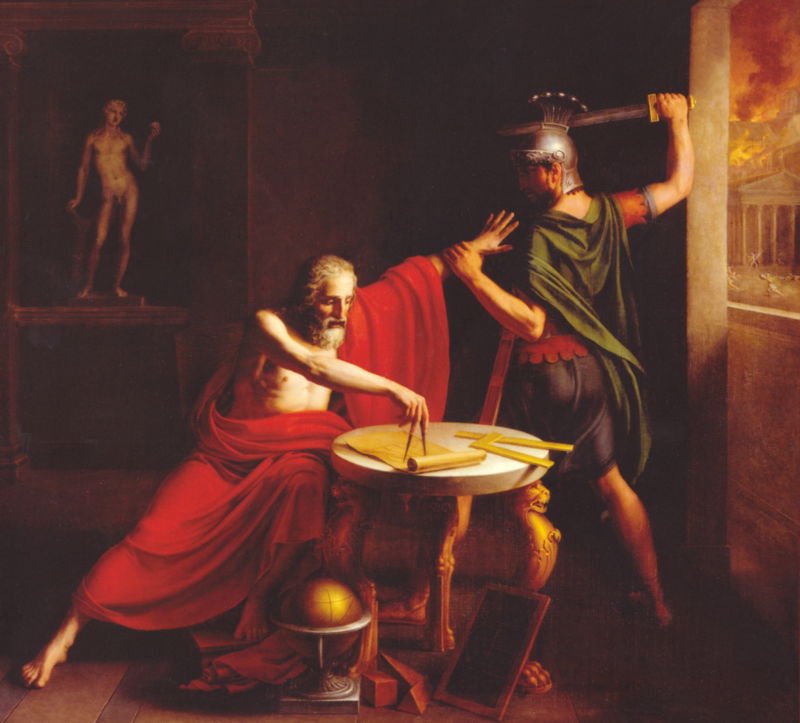
\includegraphics{Death_of_Archimedes.png}
\end{center}
%%%%%%%%% 1 OVERVIEW  %%%%%%%%%%%%%%%%%%%%
\subsection{Overview}
 
 \vspace*{-16pt}
\begin{tabular}{L{6.5in}} 
{\bf Content} \\ \hline \parskip4pt

  This part entirely studies \emph{ordered fields} which are fields $\mathbb{F}$ with 
  an ordering relation $<$ which satisfies the following properties for any $a,b,c\in\mathbb{F}$:
\begin{itemize}
  \item (Trichotomy) Exactly one of the following holds: $a < b$, $a=b$ or $b < a$.
  \item (Transitivity) $a< b$ and $b < c$ implies that $a < c$.
  \item (Addition) If $a< b$, then $a+b < a+c$.
  \item (Multiplication) If $a < b$, $0 < c$, then $ac < bc$.
\end{itemize}

 We look at the \emph{field of rational functions over the rationals, $\mathbb{Q}(x)$}

 The \emph{minimum} of a set is the least element in a set. The \emph{maximum} of
 a set is the greatest element in a set.

 A \emph{lower bound} of a set is an element which is less than every element of the
 set. 
 
 An \emph{upper bound} of a set is an element which is greater than 
 every element of the set.

 The \emph{greatest lower bound} of a set, if it exists, is the unique lower bound which is greater
 than or equal to every lower bound.

 The \emph{least upper bound} of a set, if it exists, is the unique upper bound of a set
 which is less than or equal to every upper bound.

 An \emph{Archimedean} field $\mathbb{F}$ has the property that for every 
 $x\in\mathbb{F}$ there is an integral element $n\in\mathbb{F}$ so that
 $x < n$. $\mathbb{Q}$ is Archimedean while $\mathbb{Q}(x)$ is not.

 A field is \emph{complete} if every nonempty subset of the field which is 
 bounded above has a least upper bound.

\end{tabular}

%%%%%%%%%%%%%%
\header{Summary}

In this part we explore the crucial concepts of the minimum and maximum of a set,
upper and lower bounds, and least upper bounds and greatest lower bounds. These concepts are important
in themselves in high-school mathematics. However, we take these notions a bit further to explore
the question of what makes the rational numbers and the real numbers special.
We discuss Archimedean fields, complete fields, and explore examples of these. These properties are
of crucial importance for nearly all of the algebra we do in high-school mathematics, but they are rarely
discussed except at an advanced level. We explore these properties and conclude by indicating the way in
which the real numbers is truly special - it is the unique complete ordered field.

%%%%%%%%%%%%%%
{\it Acknowledgements.}  The material in this part is inspired by the notes from courses we've taught. The textbooks used in those courses include

Hadlock, C. R. (1978). Field Theory and Its Classical Problems. Washington: Mathematical Association of America.

Madden, D. J. \& Aubrey, J. A. (2017). An introduction to proof through real analysis (1st ed.). Hoboken, NJ: Wiley.

Peressini, A. L. (2003). Mathematics for high school teachers: An advanced perspective. Prentice Hall.

%%%%%%%%%%%%%%
\newpage
\begin{bignote}[Materials]
  In this part there are six inquiries to print and give to students. They are
\begin{itemize}
  \item Opening Inquiry: $\mathbb{Q}(x)$
  \item Inquiry: Minimums and Maximums
  \item Inquiry Upper and Lower Bounds
  \item Inquiry: Least Upper Bounds and Greatest Lower Bounds
  \item Inquiry: Completeness
  \item Inquiry: Reviewing our Fields
\end{itemize}
\end{bignote}


\subsection{Opening Inquiry: $\mathbb{Q}(x)$}

\begin{task}
In $\mathbb{Q}$ and $\mathbb{R}$ we know that we have the integers as a subset. And, each positive integer can be built up by repeatedly adding 1 to itself.
That is,
\begin{align*}
  1 + 1 &= 2\\
  1+ 1 + 1 &= 3
\end{align*}
and so on. Then, once we have the positive integers, we know we have the negative integers because in a field every element has an additive inverse. 

We can do exactly the same construction in any field. That's because any arbitrary field $\mathbb{F}$ has a multiplicative identity, which we call $1$. (As we have seen,
it may actually be quite different from the number 1.) Then we can form special elements by repeatedly adding the multiplicative identity to itself over and
over. So for example, in any field we can define
\begin{align*}
  2 &= 1 + 1\\
  3 &= 1 + 1 + 1
\end{align*}
and so on. We call these elements \emph{integral elements}. In this inquiry we want to study the integral elements of a somewhat strange field - the field
of rational functions with rational coefficients. We begin by defining this field, which we denote $\mathbb{Q}(x)$.

\subsubsection{Defining $\mathbb{Q}(x)$}

First we define the set of objects $\mathbb{Q}(x)$:
\[ \mathbb{Q}(x) = \left\{ \frac{p(x)}{q(x)} \mid p(x) \text{ and }q(x)\text{ are polynomials with rational coefficients} \right\}.\]

\begin{enumerate}
  \item Which of the following are elements of $\mathbb{Q}(x)$?
    \begin{itemize}
      \item $r(x) = x^2 + 1$
      \item $s(x) = \frac{3x^2+\pi x + 1}{4x^3 + 2x^2 + x + 2}$
      \item $t(x) = \frac{x^{1/2}+2x + 1}{\frac{3}{2}x+5}$
      \item $u(x) = \frac{\frac{2}{3}x^2+2x + 1}{\frac{3}{2}x+5}$
    \end{itemize}
\end{enumerate}

We define the equality of two rational functions, as well as their sums and products, like we do with fractions. That is, given $r_1(x),r_2(x)\in\mathbb{Q}(x)$ with
$r_1(x) = \frac{p_1(x)}{q_1(x)}$ and $r_2(x) = \frac{p_2(x)}{q_2(x)}$ we define
\begin{itemize}
  \item $r_1(x)=r_2(x)$ if and only if $p_1(x)q_2(x) - q_1(x)p_2(x) = 0$
  \item $(r_1 + r_2)(x) = \frac{p_1(x)q_2(x) + q_1(x)p_2(x)}{q_1(x)q_2(x)}$
  \item $(r_1\cdot r_2)(x) = \frac{p_1(x)p_2(x)}{q_1(x)q_2(x)}$
\end{itemize}

\begin{enumerate}
    \setcounter{enumi}{1}
  \item Suppose that
    \[ r_1(x) = \frac{x^2 + \frac{1}{2}x + 2}{x+1},\quad  r_2(x) = \frac{x + 2}{x^2 +4}, \text{ and } r_3(x)=\frac{2x^2 + x + 4}{2x+2}.\]
    Is $r_1(x) = r_2(x)$? Is $r_1(x) = r_3(x)$? Is $r_2(x) = r_3(x)$?
  \item Suppose that 
    \[ r_1(x) = \frac{3x^2 + 2x + 1}{x+5} \text{ and } r_2(x) = \frac{8x + 2}{4x^2 +\frac{1}{2}}.\]
    Compute $(r_1+r_2)(x)$ and $(r_1\cdot r_2)(x)$.
\end{enumerate}

Next we define an ordering on $\mathbb{Q}(x)$ as follows: Given $r_1(x),r_2(x)\in\mathbb{Q}(x)$ with
$r_1(x) = \frac{p_1(x)}{q_1(x)}$ and $r_2(x) = \frac{p_2(x)}{q_2(x)}$, suppose that the leading coefficients of $q_1(x)$ and $q_2(x)$ are both positive. Then
\[ r_1(x) < r_2(x) \] 
if and only if the leading coefficient of 
\[ p_2(x)q_1(x) - p_1(x)q_2(x) \]
is positive. This ordering can be difficult to get a handle on. In practice you want to (a) make sure to leading coefficients in the denominator are positive, and
if not multiply by $-1/-1$ to make it so and then (b) cross multiply and subtract. Here are two examples, followed by some exercises for you to try.

\begin{example}
  Let us compare $r_1(x) = \frac{2x^2 + 11x + 1}{x+5}$ and $r_2(x) = 2x +1$. First, we observe that as a rational function $r_2(x) = \frac{2x+1}{1}$ and 
  that both $r_1(x)$ and $r_2(x)$ have positive leading coefficients in the denominator. Now we cross multiply and obtain
  \begin{align*}
    (x+5)(2x+1) &= 2x^2 + 11x + 5\\
    (1)(2x^2 + 11x + 1) = 2x^2 + 11x + 1
  \end{align*}
  We see that $(2x^2+11x + 5)-(2x^2+11x+1) = 4$ while subtracting in the other direction gives a negative. So we conclude that
  \[ \frac{2x^2+11x+1}{x+5} < 2x + 1.\]
\end{example}

\begin{example}
  Let us compare $r_1(x) = \frac{-x^2+3}{-2x+1}$ and $r_2(x) = \frac{2x+1}{2x-1}$. First, we multiply $r_1(x)$ by $-1/-1$ to rewrite it as
  $r_1(x) = \frac{x^2-3}{2x-1}$. Now we cross multiply and obtain
  \begin{align*}
    (2x-1)(x^2-3) &= 2x^3-x^2-6x +4\\
    (2x-1)(2x+1) &= 4x^2-1
  \end{align*}
  We see that $(2x^3-x^2-6x +4)- (4x^2-1) = 2x^3-5x^2-6x+3$ has positive leading coefficient. So we conclude that
  \[r_2(x) = \frac{2x+1}{2x-1} < r_1(x) = \frac{-x^2+3}{-2x+1}. \]
\end{example}

\begin{enumerate}
    \setcounter{enumi}{3}
  \item It is important to play with this ordering a bit to get used to it. Try to work through these examples in small groups. For each pair $r_1(x)$ and $r_2(x)$
    determine whether $r_1(x) < r_2(x)$, $r_1(x)=r_2(x)$ or $r_2(x) < r_1(x)$.
    \begin{enumerate}
      \item  $r_1(x) = \frac{p_1(x)}{q_1(x)} = \frac{x+5}{3x^2+x-2}$ and $r_2(x) = \frac{p_2(x)}{q_2(x)}=\frac{x+6}{3x^2+x-2}$.
      \item  $r_1(x) = \frac{p_1(x)}{q_1(x)} = \frac{x^2+5}{3x^2+x-2}$ and $r_2(x) = \frac{p_2(x)}{q_2(x)}=\frac{x+5}{3x^2+x-2}$.
      \item  $r_1(x) = \frac{p_1(x)}{q_1(x)} = \frac{x^2+5}{3x-2}$ and $r_2(x) = \frac{p_2(x)}{q_2(x)}=\frac{x^2+5}{3x^2-2}$.
      \item  $r_1(x) = \frac{p_1(x)}{q_1(x)} = \frac{x^2+5}{-3x+2}$ and $r_2(x) = \frac{p_2(x)}{q_2(x)}=\frac{x^2+5}{3x-2}$.
    \end{enumerate}
\end{enumerate}

The purpose of this opening task is to give you a sense of how the field $\mathbb{Q}(x)$ works. The fact that these operations make it an ordered field is
a theorem which is not difficult to prove, but is somewhat tedious. So here we simply state it without proof.

\begin{theorem*}
  The set of rational functions over the rationals,
\[ \mathbb{Q}(x) = \left\{ \frac{p(x)}{q(x)} \mid p(x) \text{ and }q(x)\text{ are polynomials with rational coefficients} \right\}.\]
together with the operations of addition ($+$) and multiplication ($\cdot$) defined above form a field. If we add in the ordering $<$ defined above,
$\mathbb{Q}(x)$ is an ordered field.
\end{theorem*}

We opened this inquiry by talking about integral elements. Here, in $\mathbb{Q}(x)$, the integral elements are of the form
\[ q_n(x) = n \]
for $n\in\mathbb{N}$. (Notice that these are degree 0 polynomials, and are also rational functions since $q_n(x) = \frac{n}{1}$.) As your final task in
this inquiry, prove the following facts:

\begin{enumerate}
    \setcounter{enumi}{4}
  \item Suppose that $r(x) =  x^2 + 2x + 3$. Prove that $q_{500}(x) < r(x)$
  \item Suppose that $r(x) =  2x + 3$. Prove that for any $n\in\mathbb{N}$, $q_n(x) < r(x)$.
  \item Suppose that $r(x) =  a_mx^m + a_{m-1}x_{m-1}+\cdots a_1x + a_0$ is an element
    of $\mathbb{Q}(x)$ with $m \geq 1$. Prove that if $a_m > 0$, then $q_{500}(x) < r(x)$
  \item Suppose that $r(x) =  a_mx^m + a_{m-1}x_{m-1}+\cdots a_1x + a_0$ is an element
    of $\mathbb{Q}(x)$ with $m \geq 1$. Prove that for any $n\in\mathbb{N}$, if $a_m > 0$, then $q_{n}(x) < r(x)$
\end{enumerate}

You've just shown that in $\mathbb{Q}(x)$ every polynomial with degree at least 1 and with positive leading coefficient is greater than every integral
element. 
\end{task}

Let's talk a bit more about integral elements of a field because they will play an important role below.  The idea is that every field contains
a multiplicative identity, $1$, and an addition operation $+$. So, we can add $1$ to itself as often as we like. It can get tedious to write
expressions like $1+1$, $1+1+1$, $1+1+1+1$, and so on, so we give them special names:
\begin{align*}
  2 &= 1 + 1\\
  3 &= 1 + 1 + 1\\
  4 &= 1 + 1 + 1 + 1\\
  5 &= 1 + 1 + 1 + 1 + 1
\end{align*}
and so on. In infinite fields, we can generate infinitely many integral elements in this manner. In finite fields, the expressions on the right 
are still valid - we can add 1 to itself as often as we like - but the values of those sums will cycle through the elements of the field. Notice
that in $\mathbb{Q}$ if somebody gives you any $x\in\mathbb{Q}$, no matter how large, you can always find an integral element $n$ so that
$x < n$.  Below we will call a field with this property an ``Archimedean field.'' Notice that you showed that this property does not hold in $\mathbb{Q}(x)$. 
In the inquiry above, you showed that there are some rational functions that are larger than every integral element (namely polynomials of degree at 
least 1 with positive leading coefficients). Thus, we will call $\mathbb{Q}(x)$ a \textit{non-Archimedean} field.

\section{Minimums and Maximums, Upper and Lower Bounds}

Once we have a notion of order in a field, we can talk about minimums and maximums and upper and lower bounds.

\subsection{Inquiry: Minimums and Maximums}
\begin{task}
  We haven't formally defined the notions of minimum and maximum elements of a set, but with some thought about the 
  intended meanings of these words we can come up with the definitions ourselves.
  \begin{itemize}
    \item Consider the set $S=\{3, 4, 7, 8 \}$. 
      \begin{itemize}
        \item What is the minimum of this set? Try to list two facts that make the number you chose the minimum of the set $S$.
        \item Why isn't $2$ the minimum of $S$? Why isn't $4$ the minimum of this set?
      \end{itemize}
      Try to write down the definition of the minimum of a set $S$. In a small group, discuss your definition and be prepared to share it
      with the class. Must every set have a minimum? Notice that we have talked about ``the'' minimum of a set, implying that the minimum 
      of a set $S$ is unique. Can sets have more than one minimum? Can you justify your answer?
      \begin{itemize}
        \item What is the maximum of the set $S=\{3,4,7,8\}$? Try to list two facts that make the number you chose the maximum of the set $S$.
        \item Why isn't $9$ the maximum of $S$? Why isn't $4$ the maximum of this set?
      \end{itemize}
      Try to write down the definition of the maximum of a set $S$. In a small group, discuss your definition and be prepared to share it
      with the class. Must every set have a maximum? Notice that we have talked about ``the'' maximum of a set, implying that the maximum 
      of a set $S$ is unique. Can sets have more than one maximum? Can you justify your answer?
      \begin{itemize}
        \item Suppose that $[2,3) = \{ x \in\mathbb{R} \mid 2\leq x < 3\}$. Based on your definition, what is the minimum and the maximum of $[2,3)$?
        \item Suppose that $(2,3) = \{ x \in\mathbb{R} \mid 2 < x < 3\}$. Based on your definition, what is the minimum and the maximum of $(2,3)$?
        \item Suppose that $(-\infty,3) = \{ x \in\mathbb{R} \mid x < 3\}$. Based on your definition, what is the minimum and the maximum of $(-\infty,3)$?
        \item Suppose that $[2,\infty) = \{ x \in\mathbb{R} \mid 2\leq x \}$. Based on your definition, what is the minimum and the maximum of $[2,\infty)$?
      \end{itemize}
  \end{itemize}
\end{task}

\begin{definition}
  Given a set $S$
  \begin{itemize}
    \item $m$ is a minimum of $S$ if
      \begin{itemize}
        \item $m\in S$, and 
        \item for all $x \in S$, $m\leq x$.
      \end{itemize}
    \item $M$ is a maximum of $S$ if
      \begin{itemize}
        \item $M\in S$, and 
        \item for all $x \in S$, $x\leq M$.
      \end{itemize}
  \end{itemize}
\end{definition}

\begin{lemma}
  If a set $S$ has a minimum, then it is unique.
  \label{lemma: minimums are unique}
\end{lemma}
\begin{proof}
  A good strategy for trying to prove that something is unique is to start by supposing there are two of them. So suppose that $m_1$ and $m_2$ are minimums of
  $S$. Since $m_1$ and $m_2$ are both minimums of $S$ they must both be members of $S$. 
  
  Since $m_1$ is a minimum of $S$ we must also have that $m_1 \leq x$ for every $x\in S$. But we know that $m_2\in S$, so we must have $m_1 \leq m_2$.

  Since $m_2$ is a minimum of $S$ we must also have that $m_2 \leq x$ for every $x\in S$. But we know that $m_1\in S$, so we must have $m_2 \leq m_1$.

  Thus we have $m_1\leq m_2$ and $m_2 \leq m_1$. By trichotomy, this implies that $m_1=m_2$. Thus the minimum of a set is unique.
\end{proof}

The proof that the maximum of a set is unique is similar, and we leave it as an exercise.

\subsection{Inquiry: Upper and Lower Bounds}
\begin{task}
  To illustrate the idea of upper and lower bounds, consider the following questions. Don't look up any answers on the internet, just give your best answers
  based on what you know of the world.
  \begin{itemize}
    \item Give an upper bound on the height of all humans that have ever lived.
    \item Give a lower bound on the mass of the earth.
    \item Give upper and lower bounds on the cost of raising a child.
  \end{itemize}
  Let's consider the first question for a moment. It is impossible to know how tall the tallest human ever was. Of course, we could look up the
  height of the tallest known human, but recorded history goes back only so far. And, even if the tallest person ever did in fact live during the
  period of recorded history, maybe nobody ever recorded his or her height or maybe the records were lost or forgotten. Even so, we can still give
  a reasonably good answer to the first question. For example, we can probably all agree that there was never a human who grew to be over 1 million
  feet tall. So, 1 million feet is an upper bound on the height of all humans that ever lived. Similarly, we can be confident that all humans that
  ever lived were less than 100 feet tall. So 100 feet is also an upper bound on the height of all humans that ever lived. What about 20 feet? 10 feet?
  The point is that an upper bound on a set just tells us that everything in the set is less than that value. With this discussion in mind, consider
  the other two questions and be prepared to discuss and share your answers.
  \begin{itemize}
    \item Consider the set $S = \{ 3, 5, 8, 10\}$.
      \begin{itemize}
        \item Is $15$ an upper bound of this set?
        \item Is $11$ an upper bound of this set?
        \item Is $10$ an upper bound of this set?
        \item Is $9$ an upper bound of this set?
      \end{itemize}
    \item Consider the set $[2,3) = \{ x \in\mathbb{R} \mid 2 \leq x < 3\}$.
        \begin{itemize}
          \item Is $5$ an upper bound of this set?
          \item Is $3$ an upper bound of this set?
          \item Is $3$ the maximum of this set?
          \item Is there an upper bound of this set less than $3$?
        \end{itemize}
      \item Try to complete the definition of an upper bound of a set: An element $u$ is an upper bound of
        a set $S$ if\dots
    \item Consider the set $S = \{ 3, 5, 8, 10\}$.
      \begin{itemize}
        \item Is $0$ a lower bound of this set?
        \item Is $1$ a lower bound of this set?
        \item Is $3$ a lower bound of this set?
        \item Is $4$ a lower bound of this set?
      \end{itemize}
    \item Consider the set $[2,3) = \{ x \in\mathbb{R} \mid 2 \leq x < 3\}$.
        \begin{itemize}
          \item Is $0$ a lower bound of this set?
          \item Is $1.99$ a lower bound of this set?
          \item Is $2$ a lower bound of this set?
          \item Is there a lower bound of this set greater than $2$?
        \end{itemize}
      \item Try to complete the definition of a lower bound of a set: An element $\ell$ is a lower bound of
        a set $S$ if\dots
  \end{itemize}
\end{task}

We now give the formal definitions of an upper and lower bound of a set.

\begin{definition}
  Let $\mathbb{F}$ be an ordered field and suppose that $S\subseteq \mathbb{F}$. Then
  \begin{itemize}
    \item $u$ is an upper bound of $S$ if $x \leq u$ for all $x\in S$.
    \item $l$ is a lower bound of $S$ if $l \leq x$ for all $x\in S$.
  \end{itemize}
\end{definition}

\begin{example}
  Consider the set $S = \{ x \in \mathbb{Q} \mid 2 \leq x < 3 \}$. Notice that
  $3$ is an upper bound of $S$, but so is $3.5$, $4$, and indeed any number larger
  than $3$. Similarly, $2$ is a lower bound of $\mathbb{Q}$ as is $1\frac{3}{4}$ and
  any number less than $2$. Upper bounds and lower bounds may or not be members of
  the sets they bound.
\end{example}

\subsubsection{Inquiry: Least Upper Bounds and Greatest Lower Bounds}
\begin{task}
  \begin{itemize}
    \item Some lower bounds are special in that they are the greatest lower bounds of a set. That is, not only are they lower
      bounds, but nothing larger is a lower bound.
    \item Similarly, some upper bounds are special in that they are the least upper bounds. That is, not only are they upper bounds,
      but nothing lower is an upper bound.
  \end{itemize}
  Let us explore these ideas in this inquiry.
  \begin{itemize}
    \item Consider the set $[2,3)=\{ x\in\mathbb{R} \mid 2 \leq x < 3 \}$. 
    \begin{itemize}
      \item What is the least upper bound of this set?
      \item Why isn't $2.95$ the least upper bound of this set? What about $2.999995$? 
      \item The greatest lower bound of this set is $2$. There are two ways to say this.
        \begin{itemize}
          \item First, we could express this by writing a mathematical statement which says that no number
          larger than $2$ is a lower bound of this set. That is, if $x > 2$, then $x$ is not a lower bound of $[2,3)$. What does it 
          mean to not be a lower bound of a set? Can you complete a mathematical sentence which says that no number
          larger than $2$ is a lower bound of this set? It begins ``If $x > 2$, then\dots''
        \item Second, we could express this by saying that every lower bound of this set is less than or equal to 2. Can you write a 
          mathematical statement which says this? Do you see why these two ways of expressing the idea of a greatest lower bound are
          the equivalent?
        \end{itemize}
    \end{itemize}
    \item Consider the set $[2,5]=\{ x\in\mathbb{R} \mid 2 \leq x \leq 5 \}$. 
      \begin{itemize}
        \item What is the greatest lower bound of this set? 
        \item Why isn't $2.05$ the greatest lower bound? What about $2.000001$?
        \item The least upper bound of this set is $5$. There are two ways to say this
          \begin{itemize}
            \item First, we want to write a mathematical statement which says that no number less than
          $5$ is an upper bound of this set.  That is, if $x < 5$, then $x$ is not a lower bound of $[2,5]$. What does it mean to not be
          a lower bound of a set? Can you complete a mathematical sentence which says that no number less than $5$ is an upper bound of
          this set? It begins ``If $x < 5$, then\dots''
          \item Second, we could express this by saying that every upper bound of this set is greater than or equal to 5. Can you
            write a mathematical statement which says this? Do you see why these two ways of expressing the idea of a least upper bound
            are equivalent?
          \end{itemize}
      \end{itemize}
  \end{itemize}
\end{task}

\begin{definition}
  Let $\mathbb{F}$ be an ordered field and suppose that $S\subseteq \mathbb{F}$. Then
    \item $u$ is a least upper bound of $S$ if 
      \begin{enumerate}
        \item $x \leq u$ for all $x\in S$, and
        \item If $b$ is an upper bound of $S$, then $u\leq b$. 
      \end{enumerate}
    \item $l$ is a greatest lower bound of $S$ 
      \begin{enumerate}
        \item if $l \leq x$ for all $x\in S$, and
        \item if $b$ is a lower bound of $S$, then $b \leq l$.
      \end{enumerate}
\end{definition}

\begin{example}
  Consider the set $S = \{ x \in \mathbb{Q} \mid 2 \leq x < 3 \}$. Notice that
  $3$ is an upper bound of $S$, and any other upper bound of $S$ is greater than or 
  equal to $3$. Thus, $3$ is the least upper bound of $S$. Similarly, $2$ is a lower 
  bound of $\mathbb{Q}$ and any other lower bound of $S$ must be less than or
  equal to $2$. Thus, $2$ is the greatest lower bound of $S$.  Note that a greatest 
  lower bound or least upper bound of a set may be in the set or not in the set.
\end{example}

\begin{theorem}
  If $S$ has a greatest lower bound, then it is unique. If $S$ has a least upper bound, then it is unique.
  \label{theorem: glb and lub are unqiue}
\end{theorem}
\begin{proof}
  We leave the proof of this theorem as an exercise.
\end{proof}

\subsection{The Archimedean Property and Completeness}

We have seen this definition before.

\begin{definition}
  An ordered field $\mathbb{F}$ is Archimedean if and only if for each positive $x\in\mathbb{F}$ there is an integral 
  element $k\in\mathbb{F}$ such that $x < k$.
\end{definition}

The following theorem says that in an Archimedean field, the ceiling and floor functions are well defined.

\begin{theorem}
  For each positive element $x$ in an Archimedean field $\mathbb{F}$ there is a unique integral element $n$ such that
  \[ n \leq x < n + 1.\]
  \label{theorem: archimedean implies unique integral element}
\end{theorem}
\begin{proof}
  We leave the proof as an exercise.
\end{proof}

\subsubsection{Inquiry: Completeness}
\begin{task}
  Let us consider the set
  \[ S = \{ r\in \mathbb{Q} \mid r > 0 \text{ and } r^2 < 2 \}. \]
  Note that 
  \[ \sqrt{2} = 1.414213562373095048801688724209698078569671875376948073176\dots\]
  where the decimal expansion goes on forever with no pattern. That's because $\sqrt{2}$ is irrational - it's not rational. Here we could
  write $\sqrt{2}\not\in\mathbb{Q}$ to say that $\sqrt{2}$ is not a rational number. We could be more specific and say
  $\sqrt{2}\in\mathbb{R}\setminus \mathbb{Q}$ to say that $\sqrt{2}$ is a real number but not a rational number.

  Our goal here is to figure out the least upper bound of $S$. First, for each of the numbers $r$ listed below, determine whether or not
  $r^2 < 2$.
  \begin{itemize}
    \item $r=1.414$
    \item $r=1.41421$
    \item $r=1.4142135$
    \item $r=1.414213562$
    \item $r=1.41421356237$
  \end{itemize}
  Notice that each of the numbers $r$ above satisfies $r < \sqrt{2}$. Now let's consider some numbers that are barely above $\sqrt{2}$ and
  determine whether or not they satisfy $r^2 < 2$.
  \begin{itemize}
    \item $r=1.415$
    \item $r=1.41422$
    \item $r=1.4142136$
    \item $r=1.414213563$
    \item $r=1.41421356238$
  \end{itemize}
  Complete the following sentences:
  \begin{itemize}
    \item If $r$  is less than $\sqrt{2}$, even barely, then $r^2$ \dots.
    \item If $r$  is greater than $\sqrt{2}$, even barely, then $r^2$ is\dots.
  \end{itemize}
  We now claim that $\sqrt{2}$ is an upper bound of $S$. Suppose $s\in S$ and $s > \sqrt{2}$
  \begin{itemize}
    \item There is an ordering axiom which implies that $s\cdot s > s\cdot \sqrt{2}$. Which is it?
    \item There is an ordering axiom which implies that $s\cdot \sqrt{2} > \sqrt{2}\cdot \sqrt{2}$. Which is it?
    \item There is an ordering axiom given the previous two facts implies that $s^2 > 2$. Which is it?
  \end{itemize}
  Thus, if $s\in S$, then we must have $s\leq \sqrt{2}$. So $\sqrt{2}$ is an upper bound of $S$. 
  
  We now claim that
  if $x < \sqrt{2}$, then $x$ is not an upper bound of $S$. To see this, suppose that $x < \sqrt{2}$. Then there is
  some $\epsilon > 0$ so that $x+\epsilon = \sqrt{2}$. Notice that $x < x + \epsilon/2 < \sqrt{2}$. Fill in the blanks:
  \[ (x + \epsilon/2)^2 = \underline{\hspace{2in}} < x^2 + 2x\epsilon + \epsilon^2 = (x+\epsilon)^2. \]
  But $(x+\epsilon)^2 = \underline{\hspace{1in}}$. Thus,
  \[ (x+\epsilon/2)^2 < 2. \]
  Thus $x+\epsilon/2$ is in $S$ but greater than $x$. 
  
  So, if $x<\sqrt{2}$, then $x$ is not an upper bound of $S$. So, $\sqrt{2}$ is the least upper bound of $S$. The moral of the story is
  that $S$ is a subset of $\mathbb{Q}$, but its least upper bound is not in $\mathbb{Q}$. That means that $\mathbb{Q}$ is not \emph{complete}
  in the sense defined below.
\end{task}

\begin{definition}
  An ordered field $\mathbb{F}$ is complete if and only if every subset of $\mathbb{F}$ that is bounded above has a least upper bound in 
  $\mathbb{F}$.
\end{definition}

There is nothing special about least upper bounds in this respect. We have the following theorem.

\begin{theorem}
  An ordered field $\mathbb{F}$ is complete if and only if every subset of $\mathbb{F}$ that is bounded below has a greatest lower bound
  in $\mathbb{F}$.
  \label{theorem: alternate completeness axiom}
\end{theorem}

Notice that $\mathbb{Q}$ shows that not every Archimedean field is complete. However, we have the following.

\begin{theorem}
  Any complete ordered field is Archimedean.
  \label{theorem: complete implies archimedean}
\end{theorem}
\begin{proof}
  Suppose that $\mathbb{F}$ is a complete ordered field. Suppose to the contrary that $\mathbb{F}$ is not Archimedean. Then, there is
  some $x\in \mathbb{F}$ so that no integral element $n$ is above $x$. Thus,
  \[ N = \{ n \in \mathbb{F} \mid n \text{ is an integral element} \}\]
  is bounded above by $x$. Since $N$ is a nonempty set which is bounded above and $\mathbb{F}$ is a complete field, it follows that
  $N$ has a least upper bound, say $b$. Consider $b-1$. Since $b-1 < b$ and $b$ is the least upper bound of $N$, it follows that there is
  some $n \in N$ so that $b-1 < n$. But then $b < n+1$. This is a contradiction because $n+1$ is an integral element and it is greater
  than $b$ which was suppose to be an upper bound of $N$. So, we have a contradiction and our assumption that $\mathbb{F}$ is not
  Archimedean must be false. So, we conclude that if $\mathbb{F}$ is complete, then it is Archimedean.
\end{proof}

\subsubsection{Inquiry: Reviewing our Fields}

\begin{task}
  We have just seen that every complete ordered field is Archimedean. Try to answer as many of the following questions as you can
  without looking at your notes.
  \begin{itemize}
    \item Give two examples of fields that are not ordered fields.
    \item Define what it means for a field to be Archimedean.
    \item Give an example of an ordered field that is not Archimedean.
    \item Define what it means for a field to be complete.
    \item Give an example of an Archimedean field that is not complete.
  \end{itemize}
  The real numbers $\mathbb{R}$ is a complete ordered field. In fact, it is the unique complete ordered field.
  
\end{task}

As stated in the inquiry above, we have the following theorem that makes the real numbers special. It says that there is
essentially only one complete ordered field, and it is the field of real numbers.

\begin{theorem}
  Any complete ordered field is isomorphic to the ordered field of real numbers.
  \label{theorem: reals are unique}
\end{theorem}

Again, the purpose of stating this theorem is to highlight the uniqueness of the real numbers. Essentially, the real numbers contain every number
we might need for measurement. The proof of this theorem is beyond the scope of these notes.

%%%%%%%%% 1 HOMEWORK %%%%%%%%%%%%%%%%%%%%
\newpage \subsection{Homework}  

\begin{enumerate}

\item For each of the following sets, find their minimums and maximums and greatest lower bounds and least upper bounds, if they exist.
  \begin{enumerate}
    \item $\mathbb{N}$
    \item $[0,1)$
    \item The set of irrational numbers in $[0,1]$.
  \end{enumerate}
\item Show that $0$ is the greatest lower bound of $S = \{ x \in \mathbb{R} \mid x^{-1}\in \mathbb{N}\}$.

\item Let $A$ be a set of real numbers.

\begin{enumerate}
\item Prove that if $A$ has an upper bound, then $A$ has an upper bound that
is a natural number.

\item Prove that if $A$ has a lower bound, then $A$ has a lower bound that is
an integer.

\item Prove that if $A$ has a lower bound and an upper bound, then there is a
natural number $n$ so that $n$ is an upper bound and $-n$ is a lower bound of
$A$.

\item Prove that $A$ is bounded (above and below) if and only if there is
$n\in \mathbb{N}$ so that for all $x\in A$, $-n\leq x\leq n$.

\item Prove that $A$ is bounded (above and below) if and only if there is
$n\in \mathbb{N}$ so that for all $x\in A$, $-n<x<n$.
\end{enumerate}

\item Prove that if $a\in\mathbb{R}$, then there exists $n\in \mathbb{N}$ so that $a<10^{n}$.

\item Let $a\in\mathbb{R}$.
\begin{enumerate}
\item Prove that for all $n\in\mathbb{N}$, there is $m\in \mathbb{Z}$ so that $10^{n}m\leq a\leq$ $10^{n}(m+1)$.
\item What does part a say about approximating real numbers with decimals?
\end{enumerate}

\item Let $S=\{r\in \mathbb{Q} \mid\text{there is an } n\in \mathbb{N} \text{ such that }r=\frac{10^{n}-1}{10^{n}}\}$.
\begin{enumerate}
\item Prove that $S$ has at least one element.
\item Prove that $S$ has at least one upper bound.
\item Prove that $S$ has a real number that is its least upper bound.
\item What does this tell you about $u=0.99999\dots$?
\item Can you guess what the real number $u$ is?
\end{enumerate}

\item Is $\mathbb{Q}(\sqrt{2})$ Archimedean? Is it complete?

\end{enumerate}

\section{In-Class Resources}

\newpage 
\subsection*{Opening Inquiry: $\mathbb{Q}(x)$}

\begin{task}
In $\mathbb{Q}$ and $\mathbb{R}$ we know that we have the integers as a subset. And, each positive integer can be built up by repeatedly adding 1 to itself.
That is,
\begin{align*}
  1 + 1 &= 2\\
  1+ 1 + 1 &= 3
\end{align*}
and so on. Then, once we have the positive integers, we know we have the negative integers because in a field every element has an additive inverse. 

We can do exactly the same construction in any field. That's because any arbitrary field $\mathbb{F}$ has a multiplicative identity, which we call $1$. (As we have seen,
it may actually be quite different from the number 1.) Then we can form special elements by repeatedly adding the multiplicative identity to itself over and
over. So for example, in any field we can define
\begin{align*}
  2 &= 1 + 1\\
  3 &= 1 + 1 + 1
\end{align*}
and so on. We call these elements \emph{integral elements}. In this inquiry we want to study the integral elements of a somewhat strange field - the field
of rational functions with rational coefficients. We begin by defining this field, which we denote $\mathbb{Q}(x)$.

\subsubsection{Defining $\mathbb{Q}(x)$}

First we define the set of objects $\mathbb{Q}(x)$:
\[ \mathbb{Q}(x) = \left\{ \frac{p(x)}{q(x)} \mid p(x) \text{ and }q(x)\text{ are polynomials with rational coefficients} \right\}.\]

\begin{enumerate}
  \item Which of the following are elements of $\mathbb{Q}(x)$?
    \begin{itemize}
      \item $r(x) = x^2 + 1$
        \vspace{.5in}
      \item $s(x) = \frac{3x^2+\pi x + 1}{4x^3 + 2x^2 + x + 2}$
        \vspace{.5in}
      \item $t(x) = \frac{x^{1/2}+2x + 1}{\frac{3}{2}x+5}$
        \vspace{.5in}
      \item $u(x) = \frac{\frac{2}{3}x^2+2x + 1}{\frac{3}{2}x+5}$
        \vspace{.5in}
    \end{itemize}
\end{enumerate}

We define the equality of two rational functions, as well as their sums and products, like we do with fractions. That is, given $r_1(x),r_2(x)\in\mathbb{Q}(x)$ with
$r_1(x) = \frac{p_1(x)}{q_1(x)}$ and $r_2(x) = \frac{p_2(x)}{q_2(x)}$ we define
\begin{itemize}
  \item $r_1(x)=r_2(x)$ if and only if $p_1(x)q_2(x) - q_1(x)p_2(x) = 0$
  \item $(r_1 + r_2)(x) = \frac{p_1(x)q_2(x) + q_1(x)p_2(x)}{q_1(x)q_2(x)}$
  \item $(r_1\cdot r_2)(x) = \frac{p_1(x)p_2(x)}{q_1(x)q_2(x)}$
\end{itemize}

\begin{enumerate}
    \setcounter{enumi}{1}
  \item Suppose that
    \[ r_1(x) = \frac{x^2 + \frac{1}{2}x + 2}{x+1},\quad  r_2(x) = \frac{x + 2}{x^2 +4}, \text{ and } r_3(x)=\frac{2x^2 + x + 4}{2x+2}.\]
    Is $r_1(x) = r_2(x)$? Is $r_1(x) = r_3(x)$? Is $r_2(x) = r_3(x)$?
        \vspace{1.25in}
  \item Suppose that 
    \[ r_1(x) = \frac{3x^2 + 2x + 1}{x+5} \text{ and } r_2(x) = \frac{8x + 2}{4x^2 +\frac{1}{2}}.\]
    Compute $(r_1+r_2)(x)$ and $(r_1\cdot r_2)(x)$.
        \vspace{1.25in}
\end{enumerate}

Next we define an ordering on $\mathbb{Q}(x)$ as follows: Given $r_1(x),r_2(x)\in\mathbb{Q}(x)$ with
$r_1(x) = \frac{p_1(x)}{q_1(x)}$ and $r_2(x) = \frac{p_2(x)}{q_2(x)}$, suppose that the leading coefficients of $q_1(x)$ and $q_2(x)$ are both positive. Then
\[ r_1(x) < r_2(x) \] 
if and only if the leading coefficient of 
\[ p_2(x)q_1(x) - p_1(x)q_2(x) \]
is positive. This ordering can be difficult to get a handle on. In practice you want to (a) make sure to leading coefficients in the denominator are positive, and
if not multiply by $-1/-1$ to make it so and then (b) cross multiply and subtract. Here are two examples, followed by some exercises for you to try.

\begin{example}
  Let us compare $r_1(x) = \frac{2x^2 + 11x + 1}{x+5}$ and $r_2(x) = 2x +1$. First, we observe that as a rational function $r_2(x) = \frac{2x+1}{1}$ and 
  that both $r_1(x)$ and $r_2(x)$ have positive leading coefficients in the denominator. Now we cross multiply and obtain
  \begin{align*}
    (x+5)(2x+1) &= 2x^2 + 11x + 5\\
    (1)(2x^2 + 11x + 1) = 2x^2 + 11x + 1
  \end{align*}
  We see that $(2x^2+11x + 5)-(2x^2+11x+1) = 4$ while subtracting in the other direction gives a negative. So we conclude that
  \[ \frac{2x^2+11x+1}{x+5} < 2x + 1.\]
\end{example}

\begin{example}
  Let us compare $r_1(x) = \frac{-x^2+3}{-2x+1}$ and $r_2(x) = \frac{2x+1}{2x-1}$. First, we multiply $r_1(x)$ by $-1/-1$ to rewrite it as
  $r_1(x) = \frac{x^2-3}{2x-1}$. Now we cross multiply and obtain
  \begin{align*}
    (2x-1)(x^2-3) &= 2x^3-x^2-6x +4\\
    (2x-1)(2x+1) &= 4x^2-1
  \end{align*}
  We see that $(2x^3-x^2-6x +4)- (4x^2-1) = 2x^3-5x^2-6x+3$ has positive leading coefficient. So we conclude that
  \[r_2(x) = \frac{2x+1}{2x-1} < r_1(x) = \frac{-x^2+3}{-2x+1}. \]
\end{example}

\begin{enumerate}
    \setcounter{enumi}{3}
  \item It is important to play with this ordering a bit to get used to it. Try to work through these examples in small groups. For each pair $r_1(x)$ and $r_2(x)$
    determine whether $r_1(x) < r_2(x)$, $r_1(x)=r_2(x)$ or $r_2(x) < r_1(x)$.
    \begin{enumerate}
      \item  $r_1(x) = \frac{p_1(x)}{q_1(x)} = \frac{x+5}{3x^2+x-2}$ and $r_2(x) = \frac{p_2(x)}{q_2(x)}=\frac{x+6}{3x^2+x-2}$.
        \vspace{1.5in}
      \item  $r_1(x) = \frac{p_1(x)}{q_1(x)} = \frac{x^2+5}{3x^2+x-2}$ and $r_2(x) = \frac{p_2(x)}{q_2(x)}=\frac{x+5}{3x^2+x-2}$.
        \vspace{1.5in}
      \item  $r_1(x) = \frac{p_1(x)}{q_1(x)} = \frac{x^2+5}{3x-2}$ and $r_2(x) = \frac{p_2(x)}{q_2(x)}=\frac{x^2+5}{3x^2-2}$.
        \vspace{1.5in}
      \item  $r_1(x) = \frac{p_1(x)}{q_1(x)} = \frac{x^2+5}{-3x+2}$ and $r_2(x) = \frac{p_2(x)}{q_2(x)}=\frac{x^2+5}{3x-2}$.
        \vspace{1.5in}
    \end{enumerate}
\end{enumerate}

The purpose of this opening task is to give you a sense of how the field $\mathbb{Q}(x)$ works. The fact that these operations make it an ordered field is
a theorem which is not difficult to prove, but is somewhat tedious. So here we simply state it without proof.

\begin{theorem*}
  The set of rational functions over the rationals,
\[ \mathbb{Q}(x) = \left\{ \frac{p(x)}{q(x)} \mid p(x) \text{ and }q(x)\text{ are polynomials with rational coefficients} \right\}.\]
together with the operations of addition ($+$) and multiplication ($\cdot$) defined above form a field. If we add in the ordering $<$ defined above,
$\mathbb{Q}(x)$ is an ordered field.
\end{theorem*}

We opened this inquiry by talking about integral elements. Here, in $\mathbb{Q}(x)$, the integral elements are of the form
\[ q_n(x) = n \]
for $n\in\mathbb{N}$. (Notice that these are degree 0 polynomials, and are also rational functions since $q_n(x) = \frac{n}{1}$.) As your final task in
this inquiry, prove the following facts:

\begin{enumerate}
    \setcounter{enumi}{4}
  \item Suppose that $r(x) =  x^2 + 2x + 3$. Prove that $q_{500}(x) < r(x)$
        \vspace{1.5in}
  \item Suppose that $r(x) =  2x + 3$. Prove that for any $n\in\mathbb{N}$, $q_n(x) < r(x)$.
        \vspace{1.5in}
  \item Suppose that $r(x) =  a_mx^m + a_{m-1}x_{m-1}+\cdots a_1x + a_0$ is an element
    of $\mathbb{Q}(x)$ with $m \geq 1$. Prove that if $a_m > 0$, then $q_{500}(x) < r(x)$
        \vspace{1.5in}
  \item Suppose that $r(x) =  a_mx^m + a_{m-1}x_{m-1}+\cdots a_1x + a_0$ is an element
    of $\mathbb{Q}(x)$ with $m \geq 1$. Prove that for any $n\in\mathbb{N}$, if $a_m > 0$, then $q_{n}(x) < r(x)$
        \vspace{1.5in}
\end{enumerate}

You've just shown that in $\mathbb{Q}(x)$ every polynomial with degree at least 1 and with positive leading coefficient is greater than every integral
element. 
\end{task}\newpage

\subsection{Inquiry: Minimums and Maximums}
\begin{task}
  We haven't formally defined the notions of minimum and maximum elements of a set, but with some thought about the 
  intended meanings of these words we can come up with the definitions ourselves.
  \begin{itemize}
    \item Consider the set $S=\{3, 4, 7, 8 \}$. 
      \begin{itemize}
        \item What is the minimum of this set? Try to list two facts that make the number you chose the minimum of the set $S$.
        \item Why isn't $2$ the minimum of $S$? Why isn't $4$ the minimum of this set?
      \end{itemize}
      Try to write down the definition of the minimum of a set $S$. In a small group, discuss your definition and be prepared to share it
      with the class. Must every set have a minimum? Notice that we have talked about ``the'' minimum of a set, implying that the minimum 
      of a set $S$ is unique. Can sets have more than one minimum? Can you justify your answer?
      \begin{itemize}
        \item What is the maximum of the set $S=\{3,4,7,8\}$? Try to list two facts that make the number you chose the maximum of the set $S$.
        \item Why isn't $9$ the maximum of $S$? Why isn't $4$ the maximum of this set?
      \end{itemize}
      Try to write down the definition of the maximum of a set $S$. In a small group, discuss your definition and be prepared to share it
      with the class. Must every set have a maximum? Notice that we have talked about ``the'' maximum of a set, implying that the maximum 
      of a set $S$ is unique. Can sets have more than one maximum? Can you justify your answer?
      \begin{itemize}
        \item Suppose that $[2,3) = \{ x \in\mathbb{R} \mid 2\leq x < 3\}$. Based on your definition, what is the minimum and the maximum of $[2,3)$?
        \item Suppose that $(2,3) = \{ x \in\mathbb{R} \mid 2 < x < 3\}$. Based on your definition, what is the minimum and the maximum of $(2,3)$?
        \item Suppose that $(-\infty,3) = \{ x \in\mathbb{R} \mid x < 3\}$. Based on your definition, what is the minimum and the maximum of $(-\infty,3)$?
        \item Suppose that $[2,\infty) = \{ x \in\mathbb{R} \mid 2\leq x \}$. Based on your definition, what is the minimum and the maximum of $[2,\infty)$?
      \end{itemize}
  \end{itemize}
\end{task}\newpage


\subsection{Inquiry: Upper and Lower Bounds}
\begin{task}
  To illustrate the idea of upper and lower bounds, consider the following questions. Don't look up any answers on the internet, just give your best answers
  based on what you know of the world.
  \begin{itemize}
    \item Give an upper bound on the height of all humans that have ever lived.
    \item Give a lower bound on the mass of the earth.
    \item Give upper and lower bounds on the cost of raising a child.
  \end{itemize}
  Let's consider the first question for a moment. It is impossible to know how tall the tallest human ever was. Of course, we could look up the
  height of the tallest known human, but recorded history goes back only so far. And, even if the tallest person ever did in fact live during the
  period of recorded history, maybe nobody ever recorded his or her height or maybe the records were lost or forgotten. Even so, we can still give
  a reasonably good answer to the first question. For example, we can probably all agree that there was never a human who grew to be over 1 million
  feet tall. So, 1 million feet is an upper bound on the height of all humans that ever lived. Similarly, we can be confident that all humans that
  ever lived were less than 100 feet tall. So 100 feet is also an upper bound on the height of all humans that ever lived. What about 20 feet? 10 feet?
  The point is that an upper bound on a set just tells us that everything in the set is less than that value. With this discussion in mind, consider
  the other two questions and be prepared to discuss and share your answers.
  \begin{itemize}
    \item Consider the set $S = \{ 3, 5, 8, 10\}$.
      \begin{itemize}
        \item Is $15$ an upper bound of this set?
        \item Is $11$ an upper bound of this set?
        \item Is $10$ an upper bound of this set?
        \item Is $9$ an upper bound of this set?
      \end{itemize}
    \item Consider the set $[2,3) = \{ x \in\mathbb{R} \mid 2 \leq x < 3\}$.
        \begin{itemize}
          \item Is $5$ an upper bound of this set?
          \item Is $3$ an upper bound of this set?
          \item Is $3$ the maximum of this set?
          \item Is there an upper bound of this set less than $3$?
        \end{itemize}
      \item Try to complete the definition of an upper bound of a set: An element $u$ is an upper bound of
        a set $S$ if\dots
    \item Consider the set $S = \{ 3, 5, 8, 10\}$.
      \begin{itemize}
        \item Is $0$ a lower bound of this set?
        \item Is $1$ a lower bound of this set?
        \item Is $3$ a lower bound of this set?
        \item Is $4$ a lower bound of this set?
      \end{itemize}
    \item Consider the set $[2,3) = \{ x \in\mathbb{R} \mid 2 \leq x < 3\}$.
        \begin{itemize}
          \item Is $0$ a lower bound of this set?
          \item Is $1.99$ a lower bound of this set?
          \item Is $2$ a lower bound of this set?
          \item Is there a lower bound of this set greater than $2$?
        \end{itemize}
      \item Try to complete the definition of a lower bound of a set: An element $\ell$ is a lower bound of
        a set $S$ if\dots
  \end{itemize}
\end{task}\newpage


\subsection{Inquiry: Least Upper Bounds and Greatest Lower Bounds}
\begin{task}
  \begin{itemize}
    \item Some lower bounds are special in that they are the greatest lower bounds of a set. That is, not only are they lower
      bounds, but nothing larger is a lower bound.
    \item Similarly, some upper bounds are special in that they are the least upper bounds. That is, not only are they upper bounds,
      but nothing lower is an upper bound.
  \end{itemize}
  Let us explore these ideas in this inquiry.
  \begin{itemize}
    \item Consider the set $[2,3)=\{ x\in\mathbb{R} \mid 2 \leq x < 3 \}$. 
    \begin{itemize}
      \item What is the least upper bound of this set?
      \item Why isn't $2.95$ the least upper bound of this set? What about $2.999995$? 
      \item The greatest lower bound of this set is $2$. There are two ways to say this.
        \begin{itemize}
          \item First, we could express this by writing a mathematical statement which says that no number
          larger than $2$ is a lower bound of this set. That is, if $x > 2$, then $x$ is not a lower bound of $[2,3)$. What does it 
          mean to not be a lower bound of a set? Can you complete a mathematical sentence which says that no number
          larger than $2$ is a lower bound of this set? It begins ``If $x > 2$, then\dots''
        \item Second, we could express this by saying that every lower bound of this set is less than or equal to 2. Can you write a 
          mathematical statement which says this? Do you see why these two ways of expressing the idea of a greatest lower bound are
          the equivalent?
        \end{itemize}
    \end{itemize}
    \item Consider the set $[2,5]=\{ x\in\mathbb{R} \mid 2 \leq x \leq 5 \}$. 
      \begin{itemize}
        \item What is the greatest lower bound of this set? 
        \item Why isn't $2.05$ the greatest lower bound? What about $2.000001$?
        \item The least upper bound of this set is $5$. There are two ways to say this
          \begin{itemize}
            \item First, we want to write a mathematical statement which says that no number less than
          $5$ is an upper bound of this set.  That is, if $x < 5$, then $x$ is not a lower bound of $[2,5]$. What does it mean to not be
          a lower bound of a set? Can you complete a mathematical sentence which says that no number less than $5$ is an upper bound of
          this set? It begins ``If $x < 5$, then\dots''
          \item Second, we could express this by saying that every upper bound of this set is greater than or equal to 5. Can you
            write a mathematical statement which says this? Do you see why these two ways of expressing the idea of a least upper bound
            are equivalent?
          \end{itemize}
      \end{itemize}
  \end{itemize}
\end{task}\newpage

\subsection{Inquiry: Completeness}
\begin{task}
  Let us consider the set
  \[ S = \{ r\in \mathbb{Q} \mid r > 0 \text{ and } r^2 < 2 \}. \]
  Note that 
  \[ \sqrt{2} = 1.414213562373095048801688724209698078569671875376948073176\dots\]
  where the decimal expansion goes on forever with no pattern. That's because $\sqrt{2}$ is irrational - it's not rational. Here we could
  write $\sqrt{2}\not\in\mathbb{Q}$ to say that $\sqrt{2}$ is not a rational number. We could be more specific and say
  $\sqrt{2}\in\mathbb{R}\setminus \mathbb{Q}$ to say that $\sqrt{2}$ is a real number but not a rational number.

  Our goal here is to figure out the least upper bound of $S$. First, for each of the numbers $r$ listed below, determine whether or not
  $r^2 < 2$.
  \begin{itemize}
    \item $r=1.414$
    \item $r=1.41421$
    \item $r=1.4142135$
    \item $r=1.414213562$
    \item $r=1.41421356237$
  \end{itemize}
  Notice that each of the numbers $r$ above satisfies $r < \sqrt{2}$. Now let's consider some numbers that are barely above $\sqrt{2}$ and
  determine whether or not they satisfy $r^2 < 2$.
  \begin{itemize}
    \item $r=1.415$
    \item $r=1.41422$
    \item $r=1.4142136$
    \item $r=1.414213563$
    \item $r=1.41421356238$
  \end{itemize}
  Complete the following sentences:
  \begin{itemize}
    \item If $r$  is less than $\sqrt{2}$, even barely, then $r^2$ \dots.
    \item If $r$  is greater than $\sqrt{2}$, even barely, then $r^2$ is\dots.
  \end{itemize}
  We now claim that $\sqrt{2}$ is an upper bound of $S$. Suppose $s\in S$ and $s > \sqrt{2}$
  \begin{itemize}
    \item There is an ordering axiom which implies that $s\cdot s > s\cdot \sqrt{2}$. Which is it?
    \item There is an ordering axiom which implies that $s\cdot \sqrt{2} > \sqrt{2}\cdot \sqrt{2}$. Which is it?
    \item There is an ordering axiom given the previous two facts implies that $s^2 > 2$. Which is it?
  \end{itemize}
  Thus, if $s\in S$, then we must have $s\leq \sqrt{2}$. So $\sqrt{2}$ is an upper bound of $S$. 
  
  We now claim that
  if $x < \sqrt{2}$, then $x$ is not an upper bound of $S$. To see this, suppose that $x < \sqrt{2}$. Then there is
  some $\epsilon > 0$ so that $x+\epsilon = \sqrt{2}$. Notice that $x < x + \epsilon/2 < \sqrt{2}$. Fill in the blanks:
  \[ (x + \epsilon/2)^2 = \underline{\hspace{2in}} < x^2 + 2x\epsilon + \epsilon^2 = (x+\epsilon)^2. \]
  But $(x+\epsilon)^2 = \underline{\hspace{1in}}$. Thus,
  \[ (x+\epsilon/2)^2 < 2. \]
  Thus $x+\epsilon/2$ is in $S$ but greater than $x$. 
  
  So, if $x<\sqrt{2}$, then $x$ is not an upper bound of $S$. So, $\sqrt{2}$ is the least upper bound of $S$. The moral of the story is
  that $S$ is a subset of $\mathbb{Q}$, but its least upper bound is not in $\mathbb{Q}$. That means that $\mathbb{Q}$ is not \emph{complete}
  in the sense defined below.
\end{task}\newpage

\subsubsection{Inquiry: Reviewing our Fields}

\begin{task}
  We have just seen that every complete ordered field is Archimedean. Try to answer as many of the following questions as you can
  without looking at your notes.
  \begin{itemize}
    \item Give two examples of fields that are not ordered fields.
    \item Define what it means for a field to be Archimedean.
    \item Give an example of an ordered field that is not Archimedean.
    \item Define what it means for a field to be complete.
    \item Give an example of an Archimedean field that is not complete.
  \end{itemize}
  The real numbers $\mathbb{R}$ is a complete ordered field. In fact, it is the unique complete ordered field.
\end{task}


\part{Three Famous Problems about Constructible Numbers}

\begin{center}
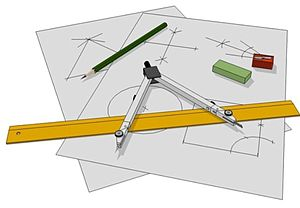
\includegraphics{straight_edge_compass_wikipedia.jpg}
\end{center}

%%%%%%%%% 1 OVERVIEW  %%%%%%%%%%%%%%%%%%%%
\subsection{Overview}
 
 \vspace*{-16pt}
\begin{tabular}{L{6.5in}} 
{\bf Content} \\ \hline \parskip4pt

\emph{Compass and straightedge constructions} are finite constructions of geometric figures
using only a compass and an unmarked straightedge.

There are three \emph{fundamental constructions} which are the only operations we
assume we can do with our straightedge and compass.

A number $a$ is said to be \emph{constructible} if and only if a line segment of
length $|a|$ can be constructed with compass and straightedge constructions.

We see that all rational numbers can be constructed, and the square root of
any constructible number can be constructed.

A \emph{Quadratic extension} of a field $\mathbb{F}$ is a field of the form
$\mathbb{F}(\sqrt{k}) = \{ a + b\sqrt{k} \mid a,b\in\mathbb{F}\}$ where $k\in\mathbb{F}$
and with appropriately defined operations.


\end{tabular}

%%%%%%%%%%%%%%
\header{Summary}

In this part we study an interesting connection between the theory of fields and
an ancient geometric technique for constructing geometric figures - compass and
straightedge constructions. We review how to accomplish many common compass and
straightedge constructions and then connect this topic to the theory of fields.
Using this connection, we give negative answers to two of three famous problems
considered by ancient Greek mathematicians.


%%%%%%%%%%%%%%
{\it Acknowledgements.}  The material in this part is inspired by the notes from courses we've taught. The textbooks used in those courses include

Hadlock, C. R. (1978). Field Theory and Its Classical Problems. Washington: Mathematical Association of America.

Madden, D. J. \& Aubrey, J. A. (2017). An introduction to proof through real analysis (1st ed.). Hoboken, NJ: Wiley.

Peressini, A. L. (2003). Mathematics for high school teachers: An advanced perspective. Prentice Hall.

%%%%%%%%%%%%%%
\newpage
\begin{bignote}[Materials]
  In this part there are 10 inquiries to print and give to students. They are
\begin{itemize}
  \item Inquiry: Bisect a line segment
  \item Inquiry: Construct Angles of $30^\circ$ and $60^\circ$
  \item Inquiry: Construct a line perpendicular to a given line
  \item Inquiry: Using Similar Triangles
  \item Inquiry: Remember the Equilateral Triangle
  \item Inquiry: Constructing Square Roots
  \item Inquiry: Am I Constructible?
  \item Inquiry: Side Length of a Cube
  \item Inquiry: $\sqrt[3]{2}$
  \item Inquiry: Remember Your Trig! (Or look it up.)
\end{itemize}
\end{bignote}

Now we turn to a collection of problems considered by ancient Greek mathematicians, namely compass-and-straightedge constructions. 
Here, by the word ``compass'' we do not mean the navigation tool! The way we're using the word, a compass is a drawing instrument 
that can be used for inscribing circles or arcs. By a ``straightedge'' we basically mean a ruler with no markings on it. 

The ancient Greeks were curious about the following question which gave rise to these problems: Given a line segment of length 1 in the plane, 
for what values of $a$ can we construct a line segment of length $a$ using compass and straightedge constructions?

The Greeks discovered how to construct sums, differences, products, ratios, and square roots of given lengths. They could also construct half of a 
given angle; that is, they could ``bisect'' any angle. We will see these constructions below, and there are many other interesting constructions
they figured out.

However, there were some constructions they could not figure out. For example, they could not figure out how to trisect an arbitrary angle. That is, they could
not construct one third of a given angle except in some particular cases. They could not ``square a circle.'' That is, they could not figure out how to 
construct a square with the same area as a given circle.  Nor could they ``double a cube.'' That is, they could not figure out how to construct the 
side of a cube whose volume would be twice the volume of a cube with a given side.

Constructions using compass and straightedge have a long history in Euclidean geometry, and they reflect the axioms of this system. However,
the restriction to using only a straightedge and compass is very artificial -- if one is actually interested in constructing a geometrical object 
for some practical purpose, then there is no reason to limit the tools to use. So why study this subject? 

Our interest comes from two directions. First, the value of the constructions themselves lie in the rich supply of problems that can be 
posed in this way. And, with regard to the constructions as solutions to these problems the important thing is to be able to analyze a 
construction to see why it works.  That is, like much of high-school geometry, the process of compass and straightedge construction is an
application of logic.

But, our primary interest in these problems comes from the fact that it took the development of the theory of fields to solve these problems. It was not until
the early 19th century that it was proved to be impossible to trisect an arbitrary angle or of double the volume of a cube using straightedge and compass 
constructions. Then in the late 19th century it was shown that $\pi$ is a transcendental number, and so it is impossible to use straightedge and compass 
to construct a square with the same area as a given circle. These proofs are beautiful uses of the theory of fields, and we will
explore them below.

\subsection{The Rules of the Game}

In the past, compasses were used in mathematics, drafting, navigation and other purposes. Physical compasses are usually made of metal or 
plastic, and consist of two parts connected by a hinge which can be adjusted to allow the changing of the radius of the circle drawn. Typically 
one part has a spike at its end, and the other part a pencil or pen. Unlike physical compasses, we will assume our compasses can be opened arbitrarily 
wide. We will also assume that our compasses have no markings on them to measure angles or anything else. 

We will assume our straightedges are infinitely long, and has no markings on them. Our straightedges can only be used to draw a line segment between 
two points or to extend an existing segment.  

Our constructions must be exact. Sometimes you'll be tempted to ``eyeball'' it by looking at the construction and guessing at its accuracy, 
or using some form of measurement, such as the units of measure on a ruler. This is forbidden, and getting close does not count as a solution.

Finally, compass and straightedge construction must have a finite number of steps.

\subsection{The Fundamental Constructions}

We begin with the three fundamental constructions with which we will build all of our more sophisticated constructions. We will assume that these
are the only operations we can perform with our straightedge and compass.

\begin{definition}[Fundamental Constructions] The following compass and straightedge constructions are known as our three fundamental constructions.
  \begin{enumerate}
    \item Given two points, we may draw a line through them, extending it indefinitely in each direction.
    \item Given two points, we may draw the line segment connecting them.
    \item Given a point and line segment, we may draw a circle with center at the point and radius equal to the length of the line segment.
  \end{enumerate}
\end{definition}

We now build up some important basic constructions using the fundamental constructions.

\begin{example}
  Using the fundamental constructions, we can bisect any angle. 
  \begin{center}
    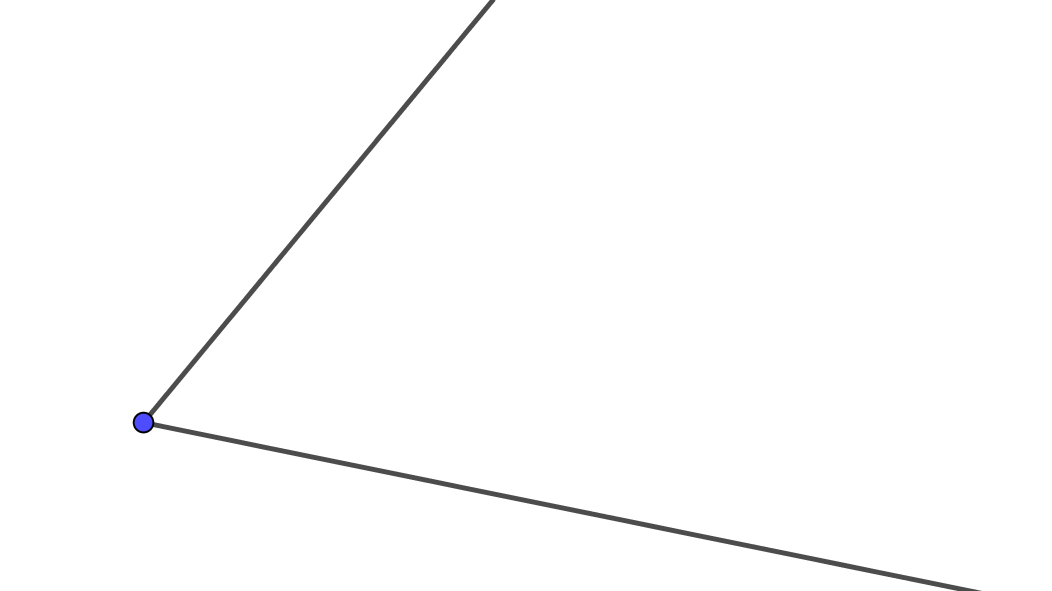
\includegraphics[scale=.75]{bisect_angle_1.png}
  \end{center}

  \begin{enumerate}
    \item We begin by opening the compass to some fixed length, putting the point of the compass at the vertex of the angle, and drawing an arc through the two 
      rays formed by the angle. This determines a point on each ray, equidistant from the vertex. (This uses the third fundamental construction.)
  \begin{center}
    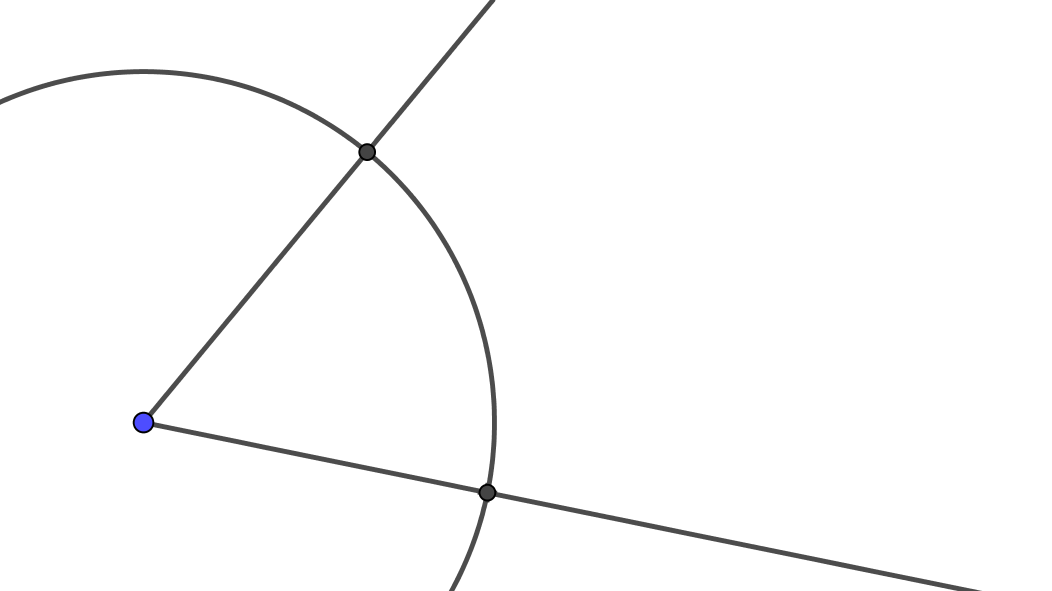
\includegraphics[scale=.75]{bisect_angle_2.png}
  \end{center}
  \item Keeping the compass at a fixed length (but perhaps different from the length in step 1), we put the compass point at each point formed in step 1
    and create two intersecting arcs between the two rays of our angle. (This uses the third fundamental construction.)
  \begin{center}
    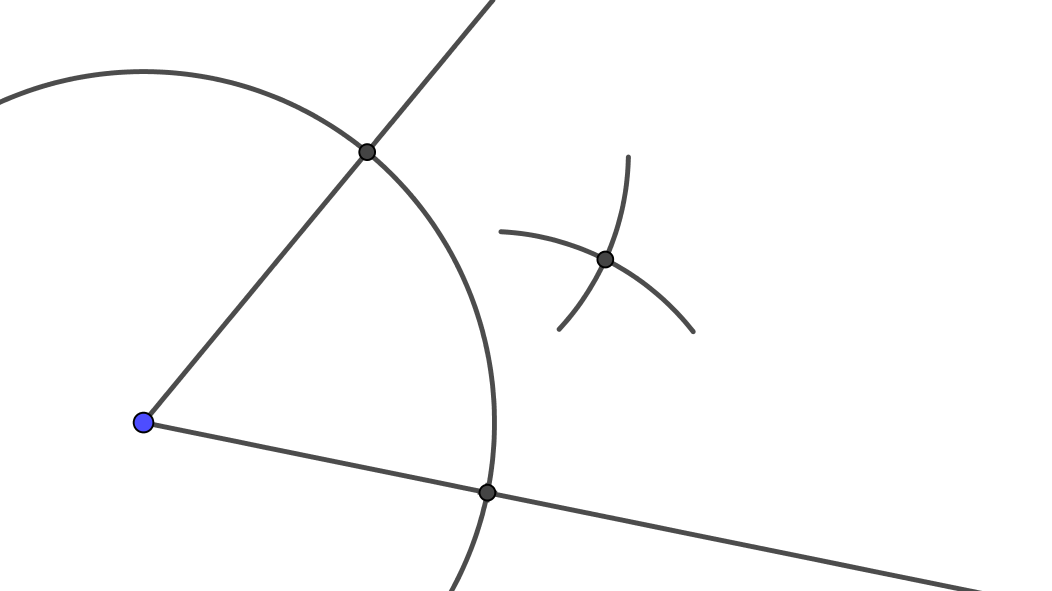
\includegraphics[scale=.75]{bisect_angle_3.png}
  \end{center}
  \item Using the straightedge, we draw a ray from the vertex of the angle through the point of intersection of the two arcs. This ray bisects the given angle.
    (This uses the first fundamental construction.)
  \begin{center}
    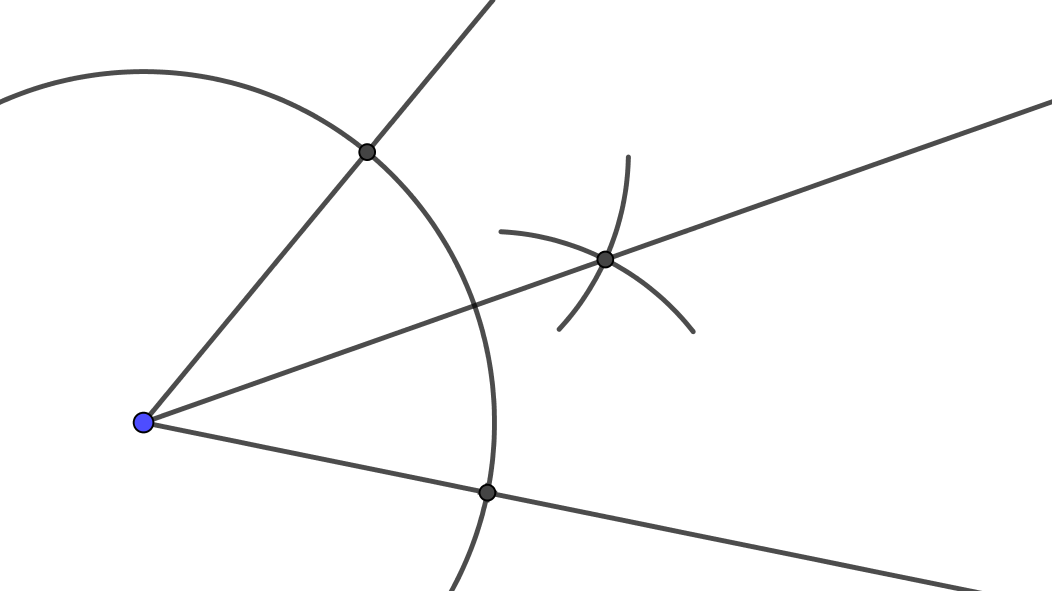
\includegraphics[scale=.75]{bisect_angle_4.png}
  \end{center}
  \end{enumerate}
\end{example}

\subsection{Inquiry: Bisect a line segment}
\begin{task}
  To bisect a line segment, follow these steps:
  \begin{enumerate}
    \item Open the compass to a width greater than half the length of the segment.
    \item Place the point of the compass at one endpoint of the segment and draw an arc which passes over the midpoint of the segment.
    \item Do the same with the point at the other endpoint of the segment without changing the width of the compass.
    \item The arcs should intersect at two points. The line between those points bisects the segment. 
  \end{enumerate}
  \begin{center}
    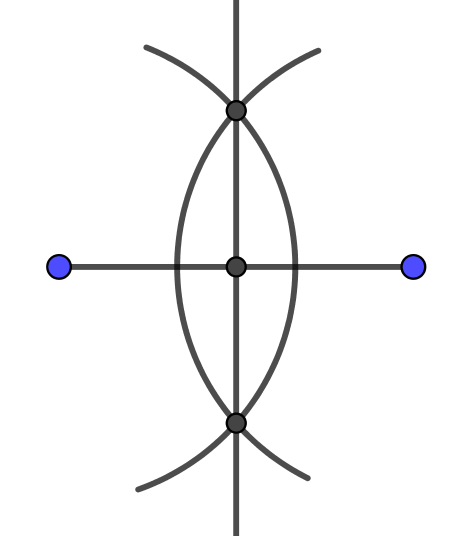
\includegraphics[scale=.75]{bisect_segment.png}
  \end{center}
\end{task}

\subsection{Inquiry: Construct Angles of $30^\circ$ and $60^\circ$}
\begin{task}

Follow these steps to construct angles of $30^\circ$ and $60^\circ$ using only the fundamental constructions.
\begin{enumerate}
  \item Using the straightedge, draw a line segment of some length.
  \item Open the compass to the length of this segment.
  \item Put the point of the compass at one end of the segment and draw an arc over the center of the line segment.
  \item Put the point of the compass at the other end of the segment and draw another arc over the center of the line segment.
  \item Draw a line segment from one end of the original segment to the intersection point of the two arcs.
\end{enumerate}

The angle between the two line segments is $60^\circ$ because the triangle formed by the two endpoints of the original line segment and the
intersection point of the arcs is an equilateral triangle. You can now construct a $30^\circ$ angle by bisecting the $60^\circ$ angle.
\end{task}

\subsection{Inquiry: Construct a line perpendicular to a given line}
\begin{task}
  Using the fundamental constructions, we can draw a line perpendicular to a given line at a point on the line. Suppose we begin with a
  line (or line segment) and a point $P$ on the line.

  \begin{enumerate}
    \item Place your compass point on $P$ and swing an arc of any size below the line that crosses the line twice. You should draw at least a semicircle. 
    \item Open the compass wider.
    \item Place the compass point where the arc crossed the line on one side and make a small arc above the line (the arc could be below the line if you prefer).
    \item Without changing the width of the compass, place the compass point where the first arc crossed the line on the other side and make another arc. 
      Your two small arcs should be intersecting.
    \item Using a straightedge, connect the intersection of the two small arcs to point $P$.
  \end{enumerate}
\end{task}

\subsection{Constructible Lengths}

Now we consider the question of what segment lengths we can construct, assuming we have in hand some given segment lengths. The next lemma essentially
says that all rational numbers are constructible.

Before stating and proving an important lemma, we have an inquiry which asks you to do a crucial step in one part of the proof.

\subsubsection{Inquiry: Using Similar Triangles}
\begin{task}
  Consider the following image:
  \begin{center}
    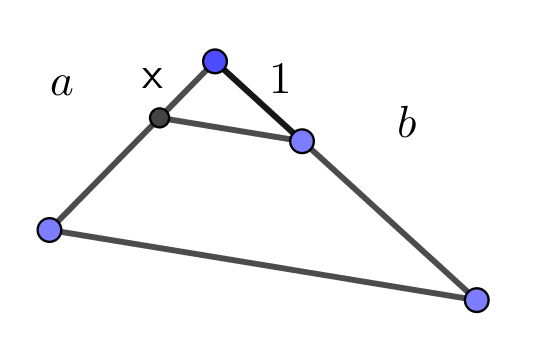
\includegraphics[scale=1]{a_over_b.png}
  \end{center}
  Here one long side of the triangle has length $a$, and a portion of that side is marked as having length $x$. Another side of the
  triangle has length $b$, and a portion of that side is marked as having length $1$. Use similar triangles to prove that in this situation $x = \frac{a}{b}$.
\end{task}

\begin{theorem}
  Given segments of length 1, $a$ and $b$, it is possible to construct segments of lengths $a+b$, $b-a$ (when $b>a$), $ab$, and $a/b$.
  \label{theorem: rational constructions}
\end{theorem}
\begin{proof}
  It is easy to see how to construct segments of length $a+b$ and $a-b$, given segments of length $a$ and $b$. For the sum, suppose we have segments of 
  length $a$ and $b$. Extend the segment of length $a$ to a line using the first fundamental construction. Then set the compass with to the length $b$,
  put the point at one endpoint of the segment of length $a$, and use the compass mark a point on the line a distance of $b$ from that endpoint in the direction
  opposite the other endpoint. The resulting long segment has length $a+b$.
  \begin{center}
    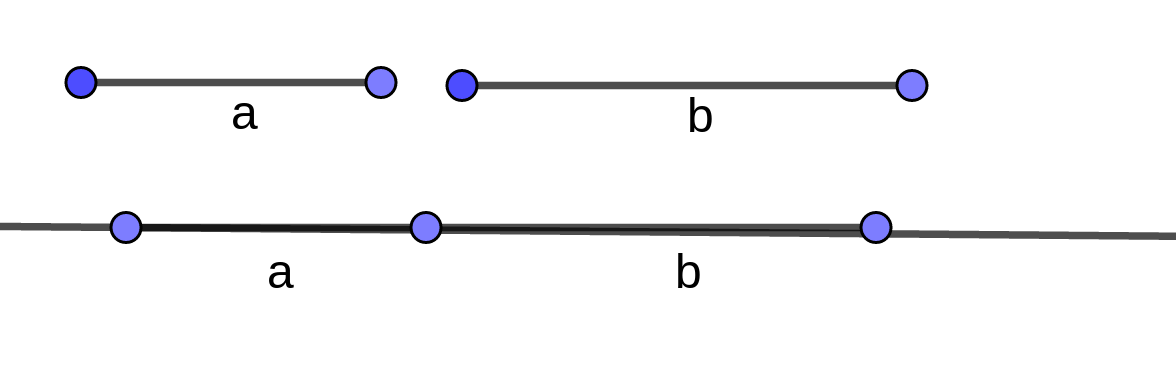
\includegraphics[scale=.1]{a_plus_b.png}
  \end{center}
  For $b-a$ when $b>a$, draw a segment of length $a$ starting from one endpoint of the segment of length $b$, toward the other endpoint of that 
  segment. What's left is a segment of length $b-a$.
  \begin{center}
    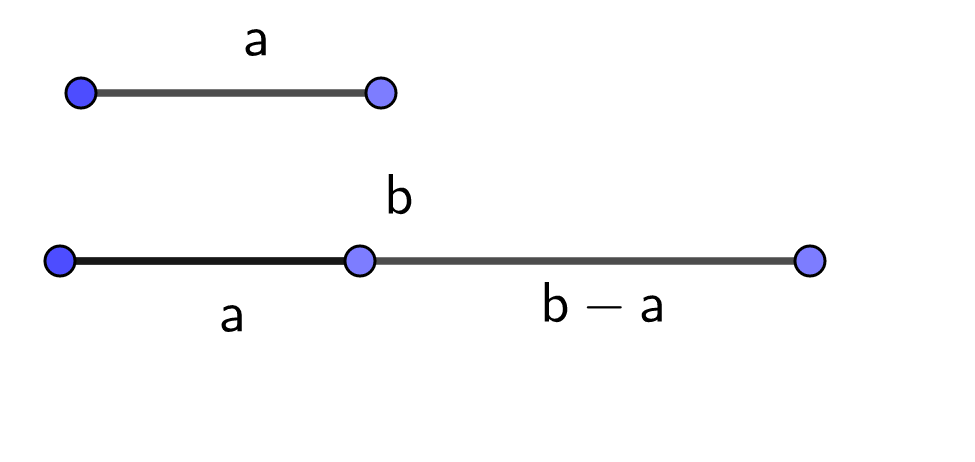
\includegraphics[scale=.1]{b_minus_a.png}
  \end{center}
  Now suppose that we have given segments of lengths $a$ and $b$. How can we construct a segment of length $ab$? This is a little more involved and we will
  do it in multiple steps. First, we pick a point and draw segments of length $a$ and length $1$ emanating from that point with some angle $\theta$ between
  them with $0^\circ < \theta < 180^\circ$
  \begin{center}
    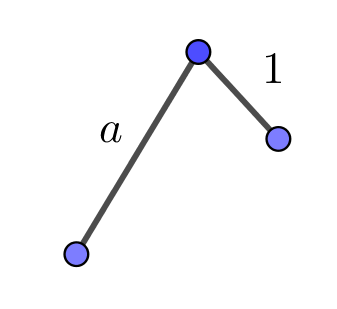
\includegraphics[scale=.75]{ab_1.png}
  \end{center}
  Now we construct two segments. One segment joints the two non-overlapping endpoints of our segment of length $a$ and our segment of length $1$. We also construct
  a segment of length $b$ adjacent to the segment of length $1$ and along the line determined by that segment.
  \begin{center}
    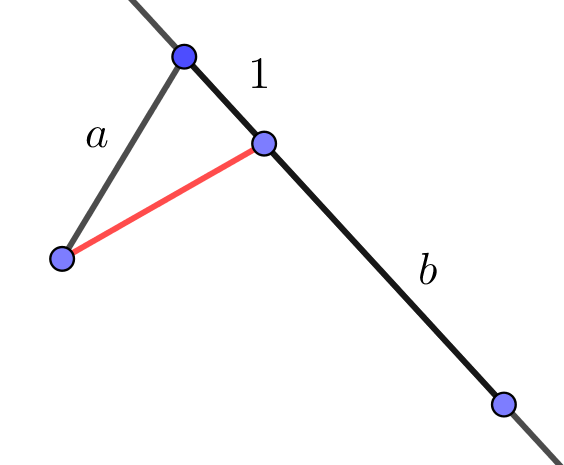
\includegraphics[scale=.75]{ab_2.png}
  \end{center}
  \begin{center}
    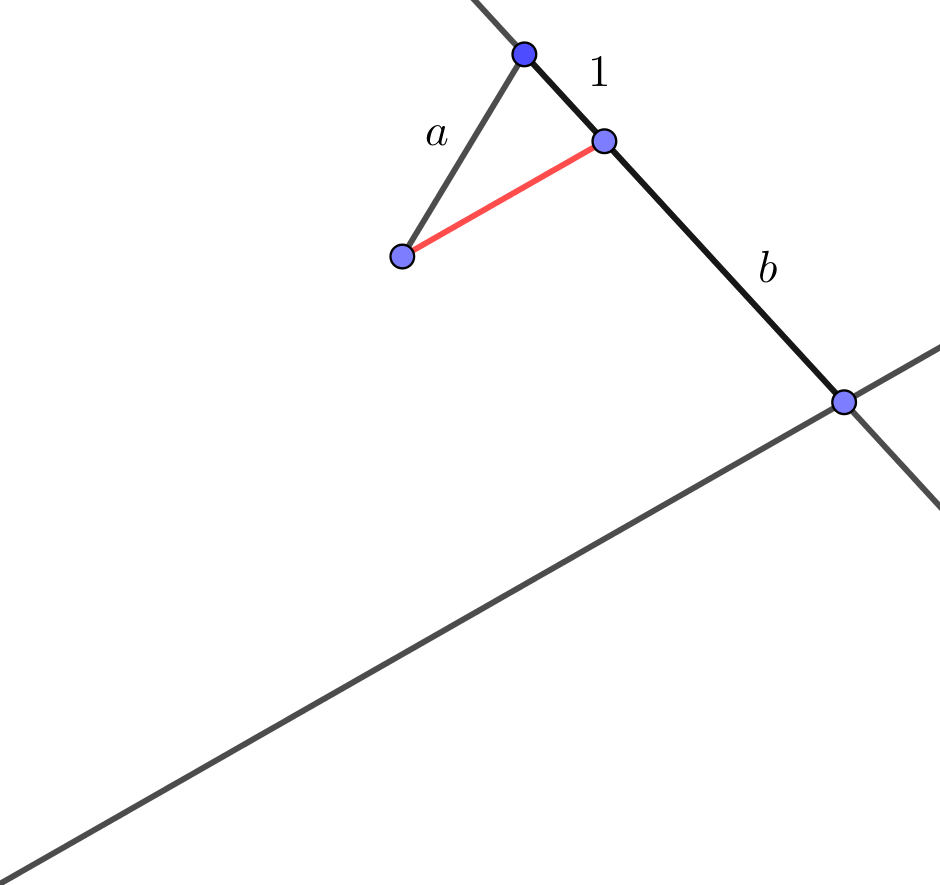
\includegraphics[scale=.75]{ab_3.png}
  \end{center}
  \begin{center}
    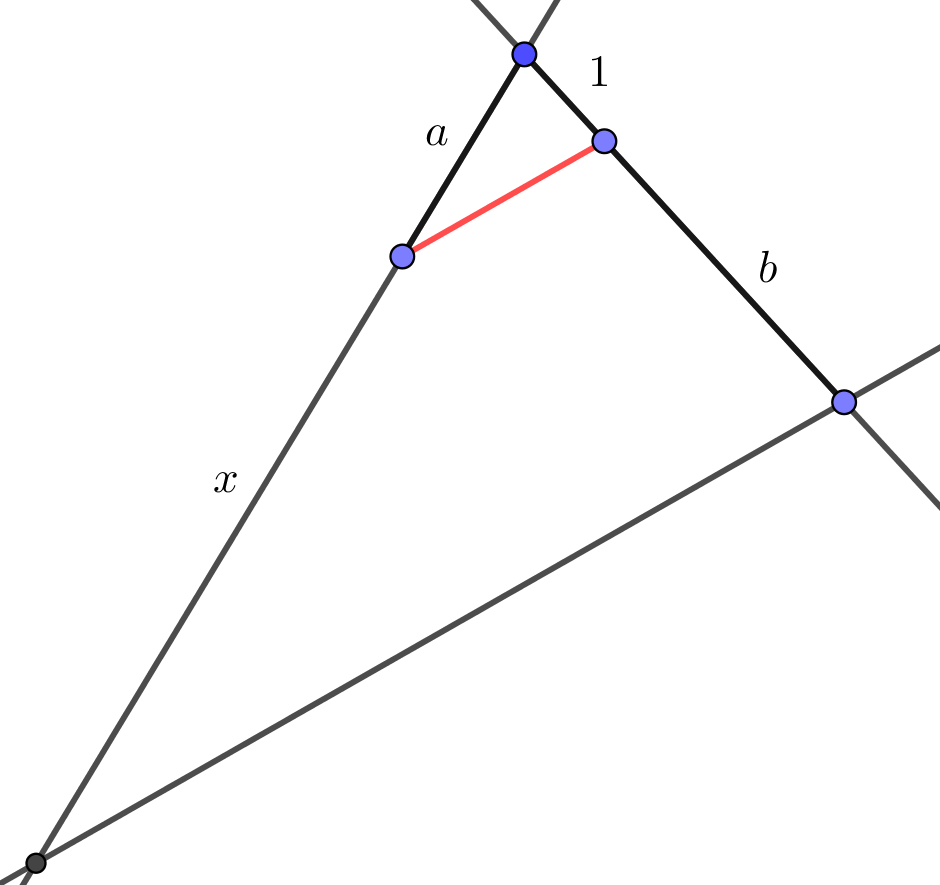
\includegraphics[scale=.75]{ab_4.png}
  \end{center}
  This shows that a segment of length of $ab$ can be constructed if we are given segments of length $a$, $b$, and $1$. As for $a/b$, the diagram
  in the inquiry above shows that a segment of length $a/b$ can be constructed.
  \begin{center}
    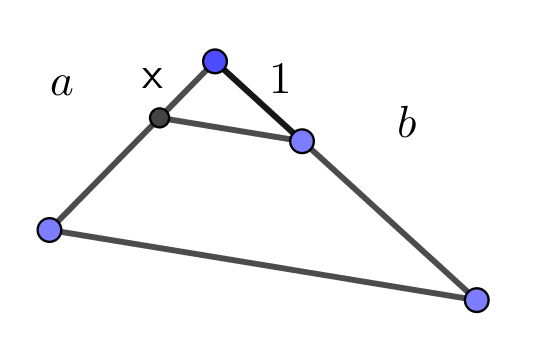
\includegraphics[scale=1]{a_over_b.png}
  \end{center}
  To complete the proof for this case, you must tie up two loose ends. First, explain how to construct this diagram using the fundamental
  constructions. Second, the diagram assumes that $b>1$. We need a diagram which handles the case $b \leq 1$. The tying of these loose ends
  is left to the reader.
\end{proof}

\begin{definition}
  A real number $a$ is constructible if given initially a segment of length $1$, it is possible to construct a segment of length $|a|$.
\end{definition}

This definition together with Theorem \ref{theorem: rational constructions} allow us to conclude that every rational number is constructible. How is this?
It should be clear that if $1$ is constructible, then so is $2$. After all, it's just $1+1$, and if we can construct a segment of length one, then
we can construct two of them side-by-side. And similarly, we can construct segments with the length of any positive natural number. This allows us
to conclude that every integer is constructible. But ratios of constructible numbers are constructible, so we get that every rational number is 
constructible. So, we have that if $1$ is constructible, then so is every natural number. Well, is $1$ a constructible length? Well, recall that our
straightedge is not a ruler - there are no distance marks. In particular, the length of ``$1$'' is not given to us. We are allowed to decide it. That is,
we are free to just create a segment of any length and call it our unit length. Then every other length is measured relative to that. We can create
a segment twice its length, three times its length,etc. Then we're off to the races and we can construct any rational length.

This is all great, but suggests the question of whether or not some non-rational numbers are constructible.  The answer is yes, but remember that to 
show that a particular non-rational number is constructible, we have to construct a line segment of that length.

\subsubsection{Inquiry: Remember the Equilateral Triangle}
\begin{task}
  Above we showed that we could construct angles of $60^\circ$ and $30^\circ$. We did that by
  \begin{enumerate}
    \item constructing an equilateral triangle, and then
    \item bisecting one of the angles in the triangle.
  \end{enumerate}
  Can we generate any constructible numbers from this construction? Use your knowledge of compass and straightedge constructions and trigonometry
  to find some non-rational constructible numbers from this example.
\end{task}

\subsubsection{Inquiry: Constructing Square Roots}

\begin{task}
  Here we suppose that we are given segments of length $1$ and length $a$, and we construct a segment of length $\sqrt{a}$. To do so, follow these
  steps.
  \begin{enumerate}
    \item Construct a segment of length $a+1$. Let $P$ be the point at which the segment of length $a$ meets the segment of length $1$.
  \begin{center}
    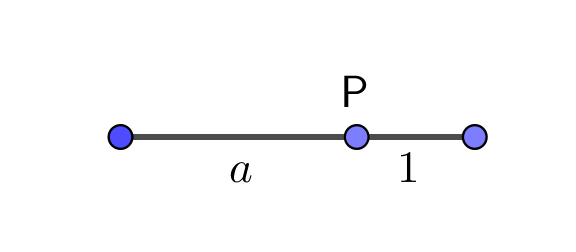
\includegraphics[scale=.75]{square_roots_1.png}
  \end{center}
    \item At point $P$ construct a line $\ell$ perpendicular to the segment.
    \item Bisect the segment, and mark its midpoint.
  %\begin{center}
  %  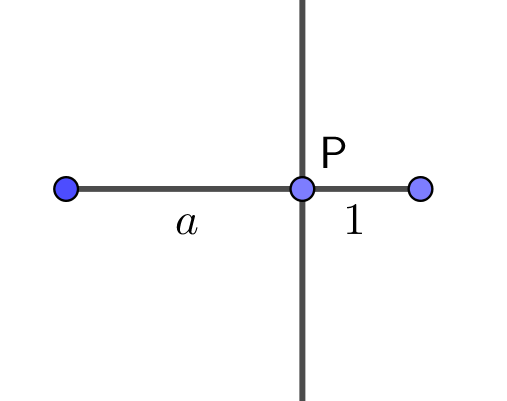
\includegraphics[scale=.75]{square_roots_2.png}
  %\end{center}
    \item Place the point of the compass at the midpoint of the segment, open the compass to half the width of the segment, and draw a circle 
      centered at the midpoint whose radius is half the length of the segment.
    \item The circle intersects the perpendicular bisector $\ell$ at two points. Pick one of them to work with, and let's call it $Q$.
  \begin{center}
    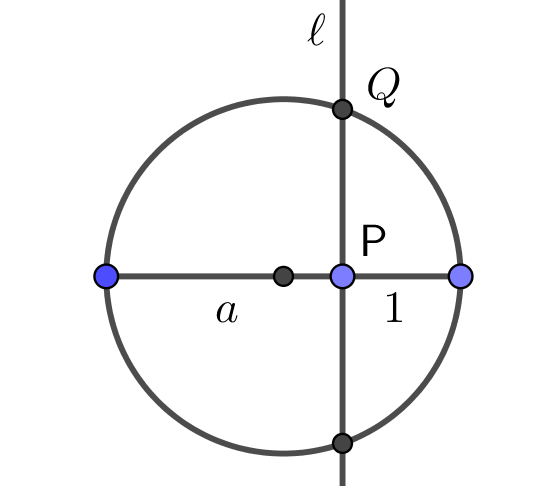
\includegraphics[scale=.75]{square_roots_3.png}
  \end{center}
    \item Let $x$ be the distance from one endpoint of the segment to $Q$ and let $y$ be the distance from $Q$ to the other endpoint. Let $z$ be
      the distance from the segment to $Q$.
  \begin{center}
    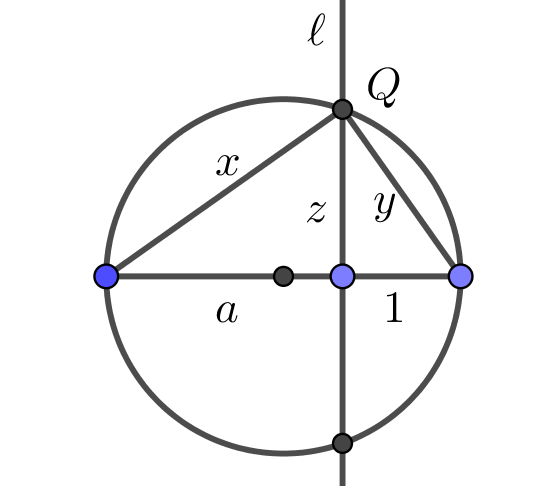
\includegraphics[scale=.75]{square_roots_4.png}
  \end{center}
    \item There are three right triangles in your picture. Write down the corresponding three instances of the Pythagorean theorem.
    \item Use these equations to show that $z=\sqrt{a}$.
  \end{enumerate}
\end{task}

\begin{lemma}
  Given segments of length $1$ and $a$, a segment of length $\sqrt{a}$ may be constructed.
  \label{lemma: sqrt can be constructed}
\end{lemma}
\begin{proof}
  You've just proved this in the inquiry above.
\end{proof}

Notice that, for example, since 1 is constructible, so is 2. This theorem allows us to conclude that $\sqrt{2}$ is constructible. So is
$\sqrt{3}, \sqrt{5}$, etc.

\subsection{Inquiry: Am I Constructible?}
\begin{task}
  In this task, you will be able to conclude based on our previous work that some of the numbers listed are constructible. For others, you will not 
  be able to draw that conclusion. Below, we'll present a theorem that exactly characterizes which numbers are constructible and which are not. Right now
  you can only identify if something is constructible. Showing something is not constructible is harder. For each number listed below indicate ``Constructible''
  or ``No Conclusion.'' If the number is constructible, explain how you would construct it given our previous constructions.
  \begin{itemize}
    \item $100$
    \item $\frac{3}{2}$
    \item $\sqrt{7}$
    \item $\sqrt[3]{7}$
    \item $3 + \sqrt{7}$
    \item $\sqrt{3 + \sqrt{7}}$
    \item $\sqrt{\sqrt{\sqrt{3+\sqrt{7}}}}$
    \item $\sqrt[4]{3 + \sqrt{7}}$
    \item $\sqrt[5]{3 + \sqrt{7}}$
    \item $\sqrt[6]{3 + \sqrt{7}}$
    \item $\sqrt[7]{3 + \sqrt{7}}$
    \item $\sqrt[n]{3 + \sqrt{7}}$, where $n$ is even.
    \item $\sqrt[n]{3 + \sqrt{7}}$, where $n$ is odd.
    \item $\pi$
  \end{itemize}
\end{task}

\subsection{Quadratic Extensions}

Now we come to the important relationship between constructible numbers and field extensions, particularly so called ``quadratic extensions.'' First, recall
the following result.

\begin{theorem}
  If $\mathbb{F}$ is a field, then so is $\mathbb{F}(\sqrt{k})$.
  \label{theorem: quadratic extensions of fields are fields}
\end{theorem}
\begin{proof}
  This was proved as homework problem \ref{homework: quadratic extensions are fields} above.
\end{proof}

First we give a sufficient condition for a number to be constructible.

\begin{theorem}
  A number $a$ is constructible if there is a finite sequence of fields $\mathbb{Q} = \mathbb{F}_0 \subset \mathbb{F}_1\subset \dots \subset \mathbb{F}_N$ with
  $a\in\mathbb{F}_N$ and such that for each $j$, $0\leq j \leq N-1$, $\mathbb{F}_{j+1}$ is a quadratic extension of $\mathbb{F}_j$.
  \label{theorem: constructible if in sequence of quadratic extensions}
\end{theorem}
\begin{proof}
  The proof of this is by induction on $N$. First consider the case where $N=0$. Since $\mathbb{F}_0=\mathbb{Q}$ and we know that every rational number
  is constructible, it follows that the theorem is true for $N=0$. Suppose now that we have a sequence of field extensions
  \[ \mathbb{Q} = \mathbb{F}_0 \subset \mathbb{F}_1\subset \dots \subset \mathbb{F}_N \]
  and that each $j$, $0\leq j \leq N-1$, $\mathbb{F}_{j+1}$ is a quadratic extension of $\mathbb{F}_j$. Suppose further that
  every number in $\mathbb{F}_N$ is constructible, and that $\mathbb{F}_{N+1}$ is a quadratic extension of $\mathbb{F}_N$. In particular, let us suppose that
  $F_{N+1}=\mathbb{F}_N(\sqrt{k})$ where $k \in \mathbb{F}_N$. Suppose that $a \in \mathbb{F}_{N+1}$. Then 
  \[ a = b + c\sqrt{k}\]
  where $b,c\in\mathbb{F}_N$. By hypothesis, every number in $\mathbb{F}_N$ is constructible. So $b$ and $c$ are constructible. Since $k\in\mathbb{F}_N$ it is also
  constructible. We know that we can construct the square root of any constructible number, so it follows that $\sqrt{k}$ is constructible. Products of
  constructible numbers are constructible, so $c\sqrt{k}$ is constructible. Sums of constructible numbers are constructible, so 
  \[ a = b + c\sqrt{k} \]
  is constructible. It follows then that every number in $\mathbb{F}_{N+1}$ is constructible. 
  
  Therefore it follows by induction that for any $N$ if there is a finite sequence of fields 
  $\mathbb{Q} = \mathbb{F}_0 \subset \mathbb{F}_1\subset \dots \subset \mathbb{F}_N$ 
  such that for each $j$, $0\leq j \leq N-1$, $\mathbb{F}_{j+1}$ is a quadratic extension of $\mathbb{F}_j$ and $a\in\mathbb{F}_N$, then $a$ is constructible. 
\end{proof}

\begin{definition}
  If $\mathbb{F}$ is a field, the plane of $\mathbb{F}$ will denote the set of all points $(x,y)$ in the Cartesian plane so that $x$ and $y$ are 
  in $\mathbb{F}$. By a line in $\mathbb{F}$ we mean a line passing through two points in the plane of $\mathbb{F}$. By a circle in $\mathbb{F}$ we 
  mean a circle with both its center and some point on its circumference in the plane of $\mathbb{F}$.
\end{definition}

Note that any fundamental construction using only points in the plane of a field $\mathbb{F}$ involves the construction of a line, line segment, 
or a circle in $\mathbb{F}$. To see this, recall the three fundamental constructions:
  \begin{enumerate}
    \item Given two points, we may draw a line through them, extending it indefinitely in each direction.
    \item Given two points, we may draw the line segment connecting them.
    \item Given a point and line segment, we may draw a circle with center at the point and radius equal to the length of the line segment.
  \end{enumerate}
If we are using only points in the plane of $\mathbb{F}$, then, in particular, the two points we start with in the first two fundamental constructions
must be points in the plane of $\mathbb{F}$. Thus the line or line segment constructed is in $\mathbb{F}$, as defined above. What about the third
fundamental construction? In this case, the center of the circle $(x,y)$ must be in the plane of $\mathbb{F}$ and the length of the line segment $r$ 
that determines the radius must be in $\mathbb{F}$. But then the point $(x+r,y)$ is on the circle and is also in the plane of $\mathbb{F}$.

\begin{lemma}
  Every line in $\mathbb{F}$ can be represented by an equation of the form $ax+by+c = 0$ with $a,b,c\in\mathbb{F}$
  \label{lemma: line in F}
\end{lemma}
\begin{proof}
  Suppose that $(x_1,y_1)$ and $(x_2,y_2)$ are points on a line in $\mathbb{F}$ and that these two points are in the plane of $\mathbb{F}$ so that
  $x_1, x_2,y_1,y_2$ are all in $\mathbb{F}$.
  Then, if the line is not vertical, then the slope of the line is
  \[ m = \frac{y_2-y_1}{x_2-x_1}. \]
  That number $m$ is in $\mathbb{F}$ if all of $x_1, x_2, y_1$, and $y_2$ are. The point-slope equation of the line is then
  \[ y-y_1 = m(x-x_1).\]
  We can rewrite this as $ax+by+c=0$ where $a=m$, $b=-1$, and $c=y_1-x_1$, and these numbers $a,b,c$ are all in $\mathbb{F}$ if $x_1, x_2, y_1$, and $y_2$
  are. If the line is vertical, then both of the points are of the form $(c,y_1)$, $(c,y_2)$ for some fixed $c$ in the $x$-coordinate and the equation of
  the line is $x=c$, or, if you like, $x-c=0$.
\end{proof}

\begin{lemma}
  Every circle in $\mathbb{F}$ can be represented by an equation of the form $x^2 + y^2 + ax + by +c = 0$ with $a,b,c\in\mathbb{F}$.
  \label{lemma: circle in F}
\end{lemma}
\begin{proof}
  The proof of this is the same idea as the proof of Lemma \ref{lemma: line in F}. We start with the center of the circle $(x_0,y_0)$ which is
  assumed to be in the plane of $\mathbb{F}$ and a point on the circumference of the circle $(x_1,y_1)$ which is also assumed to be in the 
  plane of $\mathbb{F}$. Then the radius of the circle is
  \[ r = \sqrt{(x_1-x_2)^2 + (y_1-y_2)^2}\]
  which is in not necessarily in $\mathbb{F}$, but $r^2$ definitely is. The equation of the circle is then
  \[ (x-x_0)^2 + (y-y_0)^2 = r^2.\]
  Expanding the terms on the left hand side and rearranging can clearly get us an equation of the form $x^2 + y^2 + ax + by +c = 0$ with $a,b,c\in\mathbb{F}$.
\end{proof}

\begin{theorem}
  \begin{enumerate}
    \item The point of intersection of two distinct, nonparallel lines in $\mathbb{F}$ is in the plane of $\mathbb{F}$.
    \item The points of intersection of a line in $\mathbb{F}$ and a circle in $\mathbb{F}$ are either in the plane of $\mathbb{F}$
      or in the plane of some quadratic extension of $\mathbb{F}$.
    \item The points of intersection of two circles in $\mathbb{F}$ are either in the plane of $\mathbb{F}$
      or in the plane of some quadratic extension of $\mathbb{F}$.
  \end{enumerate}
  \label{theorem: intersections}
\end{theorem}
\begin{proof}
 You can probably imagine how this is proved. For item (1) we start with two distinct, nonparallel lines. As above, these have equations
 \begin{align*}
   a_1x+b_1y+c_1&=0\\
   a_2x+b_2y+c_2&=0
 \end{align*}
 $a_1,b_1,c_1,a_2,b_2,c_2\in\mathbb{F}$. Now we solve for the intersection point. The lines must have exactly one intersection point because they are
 distinct, nonparallel lines, and that point will have coordinates which use only sums, differences, products and quotients of the coefficients. Since
 the coefficients are in $\mathbb{F}$ and $\mathbb{F}$ is a field, it follows that each of the coordinates of the intersection point will also be
 in $\mathbb{F}$.

 The situation is similar for item (2), except now we have a line and a circle so our equations look like
 \begin{align*}
   a_1x+b_1y+c_1&=0\\
   x^2 + y^2 + a_2x + b_2y +c_2 &= 0
 \end{align*}
 with $a_1,b_1,c_1,a_2,b_2,c_2\in\mathbb{F}$. If we simultaneously solve these two equations we'll use all ($+$, $-$, $\cdot$, $/$) of our arithmetic operations
 but we will also likely have to do a square root. (You can either imagine this or really try it!) If no square roots are needed, then our intersection
 point(s) are in the plane of $\mathbb{F}$. If we do need to take a square root, then our intersection points will be in the plane of a quadratic 
 extension of $\mathbb{F}$.

 In case (3) we now have two circles and our equations look like
 \begin{align*}
   x^2 + y^2 + a_1x + b_1y +c_1 &= 0\\
   x^2 + y^2 + a_2x + b_2y +c_2 &= 0
 \end{align*}
 with $a_1,b_1,c_1,a_2,b_2,c_2\in\mathbb{F}$. It's not so bad to simultaneously solve these two equations. We start by subtracting the second equation from the
 first and we get that 
 \[ (a_1-a_2)x + (b_1-b_2)y + (c_1-c_2) = 0.\]
 So, 
 \[ y = \frac{c_2-c_1}{a_1-a_2} + \frac{b_2-b_1}{c_1-c_2}x.\]
 Now we plug this into one of our original equations to get a quadratic in $x$. We can use the quadratic formula to find either zero, one or two values of $x$.
 That means the circles intersect in zero points, one point, or two points. After we find the $x$ values we determine the $y$ values. Again, to find the
 $x$-values we just take one square root. As a result, our intersection points will either be in the plane of $\mathbb{F}$ or the plane of a 
 quadratic extension of $\mathbb{F}$.
 \end{proof}

\begin{theorem}
  The following statements are equivalent:
  \begin{enumerate}
    \item The number $a$ is constructible.
    \item There is a finite sequence of fields $\mathbb{Q} = \mathbb{F}_0 \subset \mathbb{F}_1\subset \dots \subset \mathbb{F}_N$ with
  $a\in\mathbb{F}_N$ and such that for each $j$, $0\leq j \leq N-1$, $\mathbb{F}_{j+1}$ is a quadratic extension of $\mathbb{F}_j$.
  \end{enumerate}
  \label{theorem: constructible iff in sequence of quadratic extensions}
\end{theorem}
\begin{proof}
  We've already proved that (2) implies (1) above. And, we've done most of the hard work for (1) implies (2). To see that (1) implies (2),
  suppose that $a$ is constructible. That means there was some finite sequence of fundamental constructions that resulted in the construction
  of a segment of length $a$. We start with a segment of length $1$ whose endpoints we assume to have coordinates $(0,0)$ and $(1,0)$. After the
  first fundamental construction we produce a line segment, line, or circle in the plane of $\mathbb{Q}$ or in the plane of some
  quadratic extension of $\mathbb{Q}$. At each stage we produce new points by intersecting our existing constructions with our new constructed
  objects. These intersection points are either in the plane of the field we are working over, or in the plane of some quadratic extension of that
  field. Since our construction of a segment of length $a$ must terminate after a finite number of steps, it follows that if $a$ is constructible,
  then there is a finite sequence of fields $\mathbb{Q} = \mathbb{F}_0 \subset \mathbb{F}_1\subset \dots \subset \mathbb{F}_N$ with
  $a\in\mathbb{F}_N$ and such that for each $j$, $0\leq j \leq N-1$, $\mathbb{F}_{j+1}$ is a quadratic extension of $\mathbb{F}_j$.
\end{proof}

\section{Three Famous Problems}

\subsection{Doubling a Cube}

The question we want to answer in this section is the following: Given a line segment representing the edge of a cube, is it possible 
to construct another line segment representing the edge of a cube with exactly twice the volume of the first cube? Let us explore this
question a bit in the following inquiry.

\subsubsection{Inquiry: Side Length of a Cube}
\begin{task}
  \begin{itemize}
    \item Suppose that a cube, which we'll call Cube 1, has side length $s$, what is its volume?
    \item Suppose that a second cube, which we'll call Cube 2, twice the volume of Cube 1. Write an expression for the volume of Cube 2.
    \item Write an expression for the side length of Cube 2, simplified as much as possible.
    \item Supposing $s$ is a constructible number, under other number must be constructible for the volume of Cube 2 to be constructible.
  \end{itemize}
  
\end{task}

So, to ``double a cube'' means the following: We begin with a cube whose side length $s$ we take to be a constructible number $s$. Of course, 
then the volume of the cube is $V=s^3$. When we are asked to ``double'' that cube, we are being asked to use compass and straightedge 
constructions to construct a line segment of some length $\ell$, so that $\ell^3 = 2V$, which in this case would mean $\ell^3 = 2s^3$. Of 
course, we can solve for $\ell$ and we see that we want to construct a line segment of length $\sqrt[3]{2}s$. We know that $s$ is constructible,
so we may conclude that we can double our cube if and only if $\{sqrt[3]{2}$ is constructible.

\subsubsection{Inquiry: $\sqrt[3]{2}$}
\begin{task}
  Let $\mathbb{F}$ be a field, and suppose that $k\in\mathbb{F}$. Also suppose that
  \[ \sqrt[3]{2} \in \mathbb{F}(\sqrt{k})\]
  so that $\sqrt[3]{2} = a + b\sqrt{k}$ with $a,b \in \mathbb{F}$.
  \begin{itemize}
    \item Now cube both sides of the equation above.
    \item One side of the expression should just be ``2.'' The other side will have four terms, including a term with $\sqrt{k}$ (or $k^{1/2}$) and
      a term with $k^{3/2}$. Group those two terms together and factor out a $k^{1/2}$ to obtain an equation of the form
      \[ 2 = c + d\sqrt{k}.\]
    \item Why must the coefficient of $\sqrt{k}$ be zero?
    \item Explain why this implies that $b=0$, so that $\sqrt[3]{2} = a$ for $a\in \mathbb{F}$.
  \end{itemize}
  Notice that this work shows that if
  \[ \sqrt[3]{2} \in \mathbb{F}(\sqrt{k})\]
  then in fact
  \[ \sqrt[3]{2} \in \mathbb{F}.\]
\end{task}

In the previous inquiry you've proved:

\begin{theorem}
  Let $\mathbb{F}(\sqrt{k})$ be a quadratic extension of a field $\mathbb{F}$. If $\sqrt[3]{2}$ is in $\mathbb{F}(\sqrt{k})$, then $\sqrt[3]{2}$ 
  must be in $\mathbb{F}$ itself.
  \label{theorem: cube root of 2}
\end{theorem}

\begin{theorem}
  It is impossible to double the cube.
  \label{theorem: can't double cube}
\end{theorem}
\begin{proof}
  Suppose that it were possible to double the cube. Then, as we saw above, $\sqrt[3]{2}$ would be a constructible number. By 
  Theorem \ref{theorem: constructible iff in sequence of quadratic extensions}, there is a finite sequence of fields 
  $\mathbb{Q} = \mathbb{F}_0 \subset \mathbb{F}_1\subset \dots \subset \mathbb{F}_N$ with
  $\sqrt[3]{2}\in\mathbb{F}_N$ and such that for each $j$, $0\leq j \leq N-1$, $\mathbb{F}_{j+1}$ is a quadratic extension of $\mathbb{F}_j$.
  But now we repeatedly apply Theorem \ref{theorem: cube root of 2}: Since $\sqrt[3]{2}\in\mathbb{F}_N$ and $\mathbb{F}_N = \mathbb{F}_{N-1}(\sqrt{k})$
  for some $k\in\mathbb{F}_{N-1}$, it follows by Theorem \ref{theorem: cube root of 2} that $\sqrt[3]{2} \in\mathbb{F}_{N-1}$. But
  $\mathbb{F}_{N-1} = \mathbb{F}_{N-1}(\sqrt{k})$ for some $k\in\mathbb{F}_{N-2}$. So again Theorem \ref{theorem: cube root of 2} implies that
  $\sqrt[3]{2}\in\mathbb{F}_{N-2}$. And so on until we arrive at the conclusion that $\sqrt[3]{2}\in\mathbb{Q}$. But $\sqrt[3]{2}\not\in\mathbb{Q}$ - it
  is an irrational number.
\end{proof}
\
\subsection{Trisecting an Angle}

We saw above that it is possible to bisect any angle using compass and straightedge constructions. And, it must be admitted that it is possible to
trisect \textit{some} angles. For example, we know that we can construct angles of $30^\circ$ and $60^\circ$. It follows that it is indeed possible
to trisect angles with measure $3(30^\circ) = 90^\circ$ and $3(60^\circ) = 180^\circ$. But the question here is whether or not there is a general
method for trisecting an arbitrary angle? Above we demonstrated a general method for bisecting an arbitrary angle, and that's what we want here, but
for trisecting.

It turns out that this is impossible - there is no general method for trisecting an arbitrary angle. To demonstrate this fact, we must find an angle for which
we can show that it is impossible trisect that angle with compass and straightedge constructions. 

Here we will show that it is impossible to trisect an angle of $60^\circ$. Note that if this were possible, then it would be possible to construct a 
$20^\circ$ angle. Of course, if we could construct an angle of $20^\circ$, then we would be able to construct a segment of length $\cos(20^\circ)$. That
is, if it is possible to trisect an angle of $60^\circ$ with compass and straightedge constructions, then it would be possible to construct a segment
of length $\cos(20^\circ)$ with compass and straightedge constructions, meaning that $\cos(20^\circ)$ would be a constructible number.

So, to show that it is impossible to trisect an angle of $60^\circ$ it suffices to show that $\cos(20^\circ)$ is not constructible. For this we will need
some trigonometry.

\subsubsection{Inquiry: Remember Your Trig! (Or look it up.)}
\begin{task}
  Our goal in this inquiry is to find a nice polynomial which has as one of its roots the value $\cos(20^\circ)$. We begin by considering
  \[ \cos(3\theta).\]
  Even though we really want to find out something about $\cos(20^\circ)$, we begin by considering $\cos(3\theta)$ because $3(20^\circ)=60^\circ$ and we
  know the cosine of $60^\circ$. So, we'll use trig identities to write $\cos(3\theta)$ in terms of $\cos(\theta)$.

  First let us assemble our arsenal:
      \begin{enumerate}
        \item[A.] Write down the most well know trig identity - the one that hopefully know one in class needs to look up. You know the \textit{one}.
        \item[B.] There are a few well-known version of the identify for $\cos(2\theta)$. We want the one that looks a bit like the previous identity, but
          with a minus sign. (And be sure you have the order of the subtraction correct!)
        \item[C.] Now write down the most common identity for $\sin(2\theta)$.
        \item[D.] Write down the identify for $\cos(\alpha + \beta)$.
      \end{enumerate}
  Now fill in the following steps:
  \begin{enumerate}
    \item By the sum formula for cosine (identity D above):
      \begin{align*}
       \cos(3\theta) &= \cos(2\theta + \theta)\\
                     &=\underline{\hspace{4in}}
      \end{align*}
    \item In the formula above we see an instance of $\cos(2\theta)$ and an instance of $\sin(2\theta)$. Replacing these with their equivalent
      expressions (identities B and C above) we can write:
      \[ \cos(3\theta) =\underline{\hspace{4in}} \]
    \item Simplifying the previous expression we obtain
      \[ \cos(3\theta) = \cos^{\framebox(4,6){}}\theta - \framebox(5,8){}\sin^2\theta\cos\theta\]
    \item Now use identity $A$ above to replace $\sin^2\theta$ with an expression involving $\cos^2\theta$. Doing so, we obtain
      \[ \cos(3\theta) =\underline{\hspace{4in}} \]
    \item Simplify the previous expression and fill in the boxes:
      \[ \cos(3\theta) = \framebox(5,8){}\cos^3\theta - \framebox(5,8){}\cos\theta\]
    \item Now if we set $\theta = 20^\circ$, then $\cos(3\theta) = \cos(60^\circ) = \underline{\hspace{1in}}$. Rewrite the previous
      equation but substitute $20^\circ$ for $\theta$. Since you know the value of $\cos(60^\circ)$, use that value. Just leave
      $\cos(20^\circ)$ as it is - don't try to replace that expression with a decimal value. Write
      the new equation here:
      \[ \]
    \item Now let $u = \cos(20^\circ)$ and rewrite the previous equation here:
      \[ \]
    \item Now rewrite the previous equation as a polynomial in $u$ set equal to zero:
      \begin{equation}
       \framebox(5,8){}u^{\framebox(4,6){}} - 6u - \framebox(5,8){} = 0. 
        \label{equation: cos20 polynomial}
      \end{equation}
  \end{enumerate}
  Notice that this work implies that $\cos(20^\circ)$ is a root of the polynomial on the left-hand side of Equation \ref{equation: cos20 polynomial}.
\end{task}

In the inquiry above we showed that $u = \cos(20^\circ)$ must be a solution to the equation
\[ 8u^3 - 6u - 1 = 0\]
Notice that this equation can be written
 \[ (2u)^3 - 3(2u) - 1 =0. \]
 Therefore, if we take $x = 2u$ we have the polynomial
 \[ x^3 - 3x - 1 =0. \]
 We have the following theorem about this polynomial.

\begin{theorem}
  Suppose that $k\in\mathbb{F}$ and that the field $\mathbb{F}(\sqrt{k})$ contains a root of $x^3-3x-1=0$, then so does $\mathbb{F}$.
  \label{theorem: trisecting set up}
\end{theorem}
\begin{proof}
  Suppose that $a+b\sqrt{k}\in\mathbb{F}(\sqrt{k})$ and that $a+b\sqrt{k}$ is a root of the polynomial $x^3-3x-1$. We want to prove that
  there is some root of the polynomial in $\mathbb{F}$. So if we happened to get lucky and find a root with $b=0$ then we would be done. So let 
  us suppose that $a+b\sqrt{k}\in\mathbb{F}(\sqrt{k})$ and that $a+b\sqrt{k}$ is a root of the polynomial $x^3-3x-1$ \textit{and} that $b\neq 0$. Now
  we have some work to do. We are assuming the root we are given is \textit{not} in $\mathbb{F}$ and we have to produce another root which is
  in $\mathbb{F}$. Well, we claim that in this case $-2a$ is also a root of the polynomial. Notice that since $a\in\mathbb{F}$, it follows that
  $-2a$ is also in $\mathbb{F}$. So, if we can prove that $-2a$ is also a root (in addition to $a+b\sqrt{k}$) then we will have proved our theorem.
  To prove this, let's plug in our known root to $x^3-3x-1$. So
  \[ (a+b\sqrt{k})^3 - 3(a+b\sqrt{k}) -1 = 0.\]
  Let's simplify! We have
  \begin{align*}
  (a+b\sqrt{k})^3 &= a^3 + 3a^2b\sqrt{k} + 3ab^2k + b^3k^{3/2}\\
  -3(a+b\sqrt{k}) &= -3a-3b\sqrt{k}
  \end{align*}
  Thus $(a+b\sqrt{k})^3 - 3(a+b\sqrt{k}) -1 = 0$ becomes 
  \[ (a^3 + 3a^2b\sqrt{k} + 3ab^2k + b^3k^{3/2}) + (-3a-3b\sqrt{k}) -1 = 0.\]
  On the left let's group together the terms with $\sqrt{k}$ and $k^{3/2}$:
  \[ (a^3 + 3ab^2k -3a - 1) + (3a^2b\sqrt{k} + b^3k^{3/2}-3b\sqrt{k}) = 0.\]
  We can write this as
  \[ (a^3 + 3ab^2k -3a - 1) + (3a^2b + b^3k -3b)\sqrt{k} = 0.\]
  For the expression on the left to equal zero we must have
  \begin{align*}
    3a^2b + b^3k -3b &= 0\\
    a^3 + 3ab^2k -3a - 1 &= 0
  \end{align*}
    Notice we can factor $b$ out of $3a^2b+b^2k-3b$ so that $b(3a^2 + b^2k -3) = 3$. Since we are assuming that $b\neq 0$ we must have
    that $3a^2-kb^2-3=0$. Now, notice that the only place $b$ shows up in the second equation is in the term $3ab^2k$. We can use the
    equation $3a^2-kb^2-3=0$ to write $kb^2 = 3-3a^2$ so that
    \[ a^3 + 3ab^2k -3a - 1 = 0.\]
    Becomes
    \[ a^3 + 3a(3-3a^2) -3a - 1 = 0.\]
    This simplifies to
    \[ -8a^3 + 6a - 1 = 0.\]
    We can rewrite this as
    \[ (-2a)^3 - 3(-2a) - 1 = 0.\]
    That is, $-2a$ is a solution to 
    \[ x^3 - 3x - 1 = 0. \]
    That's what we wanted to prove! Thus, we have established that whether or not $b=0$, if there is a root of $x^2-3x-1$ in the field
    $\mathbb{F}(\sqrt{k})$, then there is one in the field $\mathbb{F}$.
\end{proof}

\begin{theorem}
  It is not possible to trisect and arbitrary angle.
  \label{theorem: can't trisect arbitrary angle}
\end{theorem}
\begin{proof}
  If it were possible to trisect a $60^\circ$ angle by compass and straightedge constructions, then that would imply that
  $\cos(20^\circ)$ is constructible, and therefore that a root of 
  \[ x^3 - 3x -1 = 0 \]
  is constructible. Being a constructible number, by Theorem \ref{theorem: constructible iff in sequence of quadratic extensions}
  such a root would be in some field $\mathbb{F}_N$ where
  \[ \mathbb{Q}=\mathbb{F}_0 \subseteq \mathbb{F}_1 \subseteq \cdots \subseteq \mathbb{F}_N \]
  where for $0 \leq j \leq N-1$ each $\mathbb{F}_{j+1}$ is a quadratic extension of $\mathbb{F}_j$. But, by repeated application of
  Theorem \ref{theorem: trisecting set up}, we must have a root in $\mathbb{Q}$. So, suppose that $\frac{m}{n}$ is a rational number in 
  lowest terms which is a solution to $x^3 -3x -1 =0$. That is
  \[ \left( \frac{m}{n} \right)^3 - 3\left( \frac{m}{n} \right) - 1 = 0.\]
  So of course
  \[ \frac{m^3}{n^3} - \frac{3m}{n} - 1 = 0.\]
  Let us multiply both sides of this equation by $n^3$ to obtain
  \[ m^3 - 3mn^2 - n^3 = 0.\]
  Now we can use this equation to solve for both $m^3$ and $n^3$:
  \begin{align*}
    m^3 &= 3mn^2 -n^3 = n(3mn-n^2)\\
    n^3 &= m^3 - 3mn^2 = m(m^2-3n^2)
  \end{align*}
  Now both $m$ and $n$ have prime factors. But the second equation above tells us that if a prime $p$ divides $m$, then it divides $n^3$. And, if
  a prime divides $n^3$, then it must divide $n$. So, any prime that divides $m$ must divide $n$. Similarly, the first equation tells us that if
  a prime $q$ divides $n$, then it divides $m^3$ and therefore $m$. So any prime that divides $n$ must divide $m$. That is, $m$ and $n$ have 
  exactly the same prime factors!  Since we are assuming that $m/n$ is in lowest terms, that means that $m$ and $n$ be $\pm 1$. But, neither 
  $1$ nor $-1$ is a solution to $x^3 - 3x -1 =0$. So, we have a contradiction, and we conclude there is no rational root to this equation. Therefore
  there is no constructible root to this equation. Thus, $2\cos(20^\circ)$, which is a root of this equation, is not constructible. So
  $\cos(20^\circ)$ is not constructible.
\end{proof}

\subsection{Squaring a Circle}

The ``third'' famous Greek problem is to construct a square that has the same area as the unit circle. Of course, the unit circle has radius $r=1$ and therefore
area 
\[ A = \pi r^2 = \pi(1)^2 = \pi.\]
When we say ``construct a square,'' what we really mean is that we want to construct a line segment whose length squared is the desired area. So, in this case
what we really want to do is to construct a line segment of length $\sqrt{\pi}$. If we could construct $\sqrt{\pi}$, then we could construct $\pi$. But,
it turns out that $\pi$ is a so-called ``transcendental number.'' 

An ``algebraic'' number is a real or complex number that is the root of a nonzero polynomial equation with integer (or, equivalently, rational) coefficients. 
A number is transcendental if it is not algebraic. The numbers $\pi$ and $e$ are both transcendental. It is beyond the scope of these notes to 
show that $\pi$ is transcendental, as is the fact that transcendental numbers are not constructible. These proofs lead us back to some beautiful 
mathematics and the reader is encouraged to explore further.

\newpage\subsection{Homework}

\begin{enumerate}
  \item Construct a line parallel to a given line using compass and straightedge constructions.

  \item Consider the number $r = \sqrt[4]{13}+\frac{4}{3}\sqrt{\sqrt{6}+\sqrt{1+2\sqrt{7}}}$. Give an explicit sequence of fields
  $\mathbb{F}_0 = \mathbb{Q} \subset \mathbb{F}_1 \subset \mathbb{F}_2 \subset \dots \subset \mathbb{F}_N$ such that $r \in \mathbb{F}_N$
  and for $1 \leq j \leq N-1$ each $\mathbb{F}_{j+1}$ is a quadratic extension of its predecessor $\mathbb{F}_j$.
  %\begin{solution}
  %  The number $r \in \mathbb{F}_6$ where
  %  \begin{align*}
  %    \mathbb{F}_0 &=\mathbb{Q}\\
  %    \mathbb{F}_1 &=\mathbb{F}_0(\sqrt{7})\\
  %    \mathbb{F}_2 &=\mathbb{F}_1(\sqrt{1+2\sqrt{7}})\\
  %    \mathbb{F}_3 &=\mathbb{F}_2(\sqrt{6})\\
  %    \mathbb{F}_4 &=\mathbb{F}_3(\sqrt{\sqrt{6}+\sqrt{1+2\sqrt{7}}})\\
  %    \mathbb{F}_5 &=\mathbb{F}_4(\sqrt{13})\\
  %    \mathbb{F}_6 &=\mathbb{F}_5(\sqrt[4]{13})
  %  \end{align*}
  %\end{solution}

  \item Can the cube be ``tripled''?
  %\begin{solution}
  %  Nope, same argument as for doubled, but with $\sqrt[3]{3}$.
  %\end{solution}

  \item It is clearly possible to divide an arbitrary angle into four equal parts by repeated bisection.  Show how this may
  also be deduced algebraically from the equation relating $\cos(4\theta)$ and $\cos \theta$.
  %\begin{solution}
  %  Assume that an angle $4\theta$ is constructible. By an argument similar to what we have seen in class (i.e. by \emph{geometry},
  %  this implies that $\cos(4\theta)$ is constructible.  We also know that dividing the angle into four equal parts would be 
  %  equivalent to constructing $\cos(\theta)$. So, we argue that $\cos(\theta)$ is constructible: First, using trig identities you can show that 
  %  \[ \cos(4\theta) = 8\cos^4(\theta)-8\cos^2(\theta)+1 \]
  %  If we let $x = \cos^2(\theta)$ we obtain the equation,
  %  \[ 8x^2 - 8x + (1-\cos(4\theta) = 0\]
  %  The quadratic equation gives
  %  \[ x = \frac{8 \pm \sqrt{64 - 32(1-\cos(4\theta))}}{16} \]
  %  Notice that since $-1 \leq \cos(4\theta) \leq 1$, the discrimiant is at least zero, so the possible values for $x$ are always real 
  %  numbers.  Even more, the values of $x$ can clearly be seen to be in $\mathbb{Q}$ or a quadratic extension of $\mathbb{Q}$. Thus
  %  those possible values for $x$ are constructible.  That gives us that $\cos^2(\theta)$ is constructible, and that implies
  %  $\cos(\theta)$ is constructible.
  %\end{solution}
  \end{enumerate}

\newpage\subsection{In-Class Resources}

\subsubsection{Inquiry: Bisect a line segment}
\begin{task}
  To bisect a line segment, follow these steps:
  \begin{enumerate}
    \item Open the compass to a width greater than half the length of the segment.
    \item Place the point of the compass at one endpoint of the segment and draw an arc which passes over the midpoint of the segment.
    \item Do the same with the point at the other endpoint of the segment without changing the width of the compass.
    \item The arcs should intersect at two points. The line between those points bisects the segment. 
  \end{enumerate}
  \begin{center}
    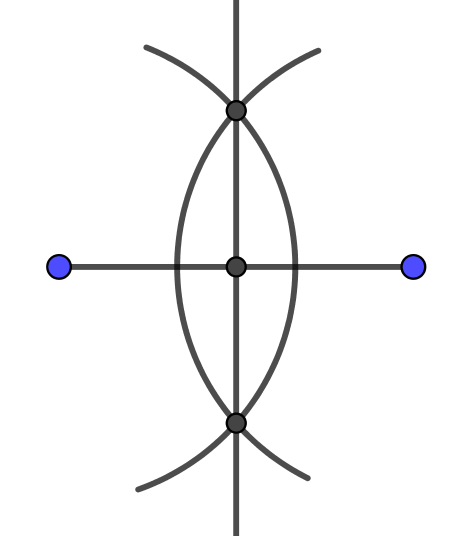
\includegraphics[scale=.75]{bisect_segment.png}
  \end{center}
\end{task}\newpage

\subsubsection{Inquiry: Construct Angles of $30^\circ$ and $60^\circ$}
\begin{task}

Follow these steps to construct angles of $30^\circ$ and $60^\circ$ using only the fundamental constructions.
\begin{enumerate}
  \item Using the straightedge, draw a line segment of some length.
  \item Open the compass to the length of this segment.
  \item Put the point of the compass at one end of the segment and draw an arc over the center of the line segment.
  \item Put the point of the compass at the other end of the segment and draw another arc over the center of the line segment.
  \item Draw a line segment from one end of the original segment to the intersection point of the two arcs.
\end{enumerate}

The angle between the two line segments is $60^\circ$ because the triangle formed by the two endpoints of the original line segment and the
intersection point of the arcs is an equilateral triangle. You can now construct a $30^\circ$ angle by bisecting the $60^\circ$ angle.
\end{task}\newpage

\subsubsection{Inquiry: Construct a line perpendicular to a given line}
\begin{task}
  Using the fundamental constructions, we can draw a line perpendicular to a given line at a point on the line. Suppose we begin with a
  line (or line segment) and a point $P$ on the line.

  \begin{enumerate}
    \item Place your compass point on $P$ and swing an arc of any size below the line that crosses the line twice. You should draw at least a semicircle. 
    \item Open the compass wider.
    \item Place the compass point where the arc crossed the line on one side and make a small arc above the line (the arc could be below the line if you prefer).
    \item Without changing the width of the compass, place the compass point where the first arc crossed the line on the other side and make another arc. 
      Your two small arcs should be intersecting.
    \item Using a straightedge, connect the intersection of the two small arcs to point $P$.
  \end{enumerate}
\end{task}\newpage

\subsubsection{Inquiry: Using Similar Triangles}
\begin{task}
  Consider the following image:
  \begin{center}
    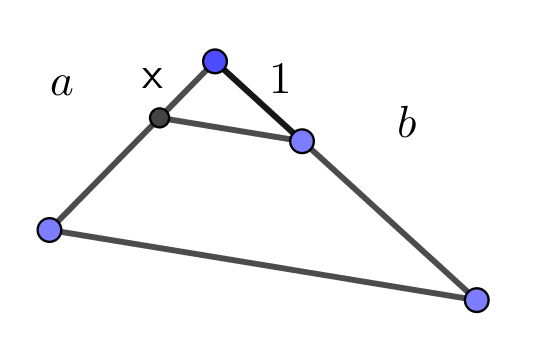
\includegraphics[scale=1]{a_over_b.png}
  \end{center}
  Here one long side of the triangle has length $a$, and a portion of that side is marked as having length $x$. Another side of the
  triangle has length $b$, and a portion of that side is marked as having length $1$. Use similar triangles to prove that in this situation $x = \frac{a}{b}$.
\end{task}\newpage

\subsubsection{Inquiry: Remember the Equilateral Triangle}
\begin{task}
  Above we showed that we could construct angles of $60^\circ$ and $30^\circ$. We did that by
  \begin{enumerate}
    \item constructing an equilateral triangle, and then
    \item bisecting one of the angles in the triangle.
  \end{enumerate}
  Can we generate any constructible numbers from this construction? Use your knowledge of compass and straightedge constructions and trigonometry
  to find some non-rational constructible numbers from this example.
\end{task}\newpage

\subsubsection{Inquiry: Constructing Square Roots}

\begin{task}
  Here we suppose that we are given segments of length $1$ and length $a$, and we construct a segment of length $\sqrt{a}$. To do so, follow these
  steps.
  \begin{enumerate}
    \item Construct a segment of length $a+1$. Let $P$ be the point at which the segment of length $a$ meets the segment of length $1$.
  \begin{center}
    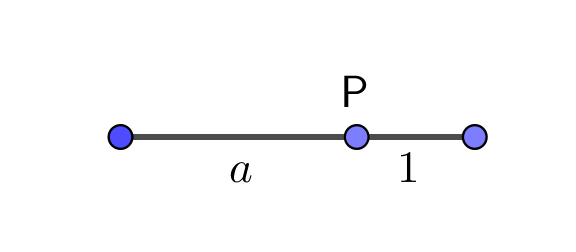
\includegraphics[scale=.75]{square_roots_1.png}
  \end{center}
    \item At point $P$ construct a line $\ell$ perpendicular to the segment.
    \item Bisect the segment, and mark its midpoint.
  %\begin{center}
  %  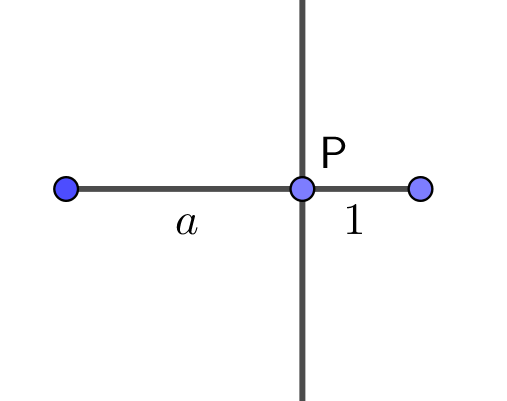
\includegraphics[scale=.75]{square_roots_2.png}
  %\end{center}
    \item Place the point of the compass at the midpoint of the segment, open the compass to half the width of the segment, and draw a circle 
      centered at the midpoint whose radius is half the length of the segment.
    \item The circle intersects the perpendicular bisector $\ell$ at two points. Pick one of them to work with, and let's call it $Q$.
  \begin{center}
    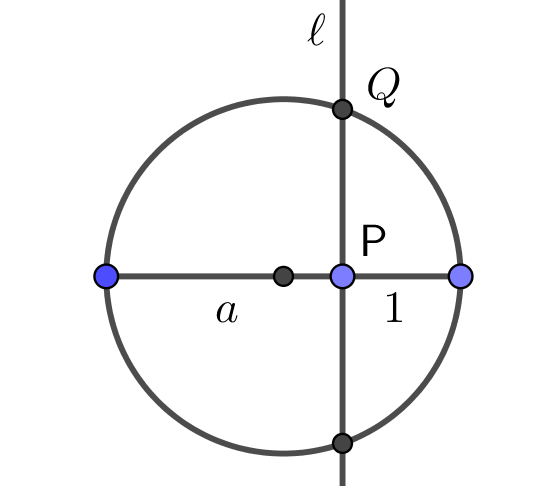
\includegraphics[scale=.75]{square_roots_3.png}
  \end{center}
    \item Let $x$ be the distance from one endpoint of the segment to $Q$ and let $y$ be the distance from $Q$ to the other endpoint. Let $z$ be
      the distance from the segment to $Q$.
  \begin{center}
    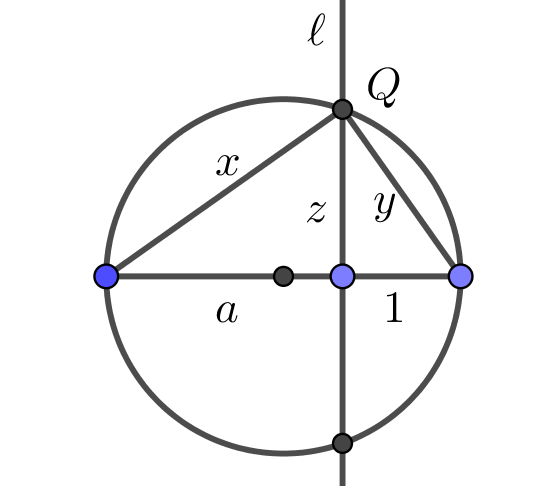
\includegraphics[scale=.75]{square_roots_4.png}
  \end{center}
    \item There are three right triangles in your picture. Write down the corresponding three instances of the Pythagorean theorem.
    \item Use these equations to show that $z=\sqrt{a}$.
  \end{enumerate}
\end{task}\newpage

\subsection{Inquiry: Am I Constructible?}
\begin{task}
  In this task, you will be able to conclude based on our previous work that some of the numbers listed are constructible. For others, you will not 
  be able to draw that conclusion. Below, we'll present a theorem that exactly characterizes which numbers are constructible and which are not. Right now
  you can only identify if something is constructible. Showing something is not constructible is harder. For each number listed below indicate ``Constructible''
  or ``No Conclusion.'' If the number is constructible, explain how you would construct it given our previous constructions.
  \begin{itemize}
    \item $100$
    \item $\frac{3}{2}$
    \item $\sqrt{7}$
    \item $\sqrt[3]{7}$
    \item $3 + \sqrt{7}$
    \item $\sqrt{3 + \sqrt{7}}$
    \item $\sqrt{\sqrt{\sqrt{3+\sqrt{7}}}}$
    \item $\sqrt[4]{3 + \sqrt{7}}$
    \item $\sqrt[5]{3 + \sqrt{7}}$
    \item $\sqrt[6]{3 + \sqrt{7}}$
    \item $\sqrt[7]{3 + \sqrt{7}}$
    \item $\sqrt[n]{3 + \sqrt{7}}$, where $n$ is even.
    \item $\sqrt[n]{3 + \sqrt{7}}$, where $n$ is odd.
    \item $\pi$
  \end{itemize}
\end{task}\newpage

\subsubsection{Inquiry: Side Length of a Cube}
\begin{task}
  \begin{itemize}
    \item Suppose that a cube, which we'll call Cube 1, has side length $s$, what is its volume?
    \item Suppose that a second cube, which we'll call Cube 2, twice the volume of Cube 1. Write an expression for the volume of Cube 2.
    \item Write an expression for the side length of Cube 2, simplified as much as possible.
    \item Supposing $s$ is a constructible number, under other number must be constructible for the volume of Cube 2 to be constructible.
  \end{itemize}
  
\end{task}\newpage

\subsubsection{Inquiry: $\sqrt[3]{2}$}
\begin{task}
  Let $\mathbb{F}$ be a field, and suppose that $k\in\mathbb{F}$. Also suppose that
  \[ \sqrt[3]{2} \in \mathbb{F}(\sqrt{k})\]
  so that $\sqrt[3]{2} = a + b\sqrt{k}$ with $a,b \in \mathbb{F}$.
  \begin{itemize}
    \item Now cube both sides of the equation above.
    \item One side of the expression should just be ``2.'' The other side will have four terms, including a term with $\sqrt{k}$ (or $k^{1/2}$) and
      a term with $k^{3/2}$. Group those two terms together and factor out a $k^{1/2}$ to obtain an equation of the form
      \[ 2 = c + d\sqrt{k}.\]
    \item Why must the coefficient of $\sqrt{k}$ be zero?
    \item Explain why this implies that $b=0$, so that $\sqrt[3]{2} = a$ for $a\in \mathbb{F}$.
  \end{itemize}
  Notice that this work shows that if
  \[ \sqrt[3]{2} \in \mathbb{F}(\sqrt{k})\]
  then in fact
  \[ \sqrt[3]{2} \in \mathbb{F}.\]
\end{task}\newpage

\subsubsection{Inquiry: Remember Your Trig! (Or look it up.)}
\begin{task}
  Our goal in this inquiry is to find a nice polynomial which has as one of its roots the value $\cos(20^\circ)$. We begin by considering
  \[ \cos(3\theta).\]
  Even though we really want to find out something about $\cos(20^\circ)$, we begin by considering $\cos(3\theta)$ because $3(20^\circ)=60^\circ$ and we
  know the cosine of $60^\circ$. So, we'll use trig identities to write $\cos(3\theta)$ in terms of $\cos(\theta)$.

  First let us assemble our arsenal:
      \begin{enumerate}
        \item[A.] Write down the most well know trig identity - the one that hopefully know one in class needs to look up. You know the \textit{one}.
        \item[B.] There are a few well-known version of the identify for $\cos(2\theta)$. We want the one that looks a bit like the previous identity, but
          with a minus sign. (And be sure you have the order of the subtraction correct!)
        \item[C.] Now write down the most common identity for $\sin(2\theta)$.
        \item[D.] Write down the identify for $\cos(\alpha + \beta)$.
      \end{enumerate}
  Now fill in the following steps:
  \begin{enumerate}
    \item By the sum formula for cosine (identity D above):
      \begin{align*}
       \cos(3\theta) &= \cos(2\theta + \theta)\\
                     &=\underline{\hspace{4in}}
      \end{align*}
    \item In the formula above we see an instance of $\cos(2\theta)$ and an instance of $\sin(2\theta)$. Replacing these with their equivalent
      expressions (identities B and C above) we can write:
      \[ \cos(3\theta) =\underline{\hspace{4in}} \]
    \item Simplify the previous expression and fill in the boxes:
      \[ \cos(3\theta) = \cos^{\framebox(4,6){}}\theta - \framebox(5,8){}\sin^2\theta\cos\theta\]
    \item Now use identity $A$ above to replace $\sin^2\theta$ with an expression involving $\cos^2\theta$. Doing so, we obtain
      \[ \cos(3\theta) =\underline{\hspace{4in}} \]
    \item Simplifying the previous expression we obtain
      \[ \cos(3\theta) = \framebox(5,8){}\cos^3\theta - \framebox(5,8){}\cos\theta\]
    \item Now if we set $\theta = 20^\circ$, then $\cos(3\theta) = \cos(60^\circ) = \underline{\hspace{1in}}$. Rewrite the previous
      equation but substitute $20^\circ$ for $\theta$. Since you know the value of $\cos(60^\circ)$, use that value. Just leave
      $\cos(20^\circ)$ as it is - don't try to replace that expression with a decimal value. Write
      the new equation here:
      \[ \]
    \item Now let $u = \cos(20^\circ)$ and rewrite the previous equation here:
      \[ \]
    \item Now rewrite the previous equation as a polynomial in $u$ set equal to zero:
      \begin{equation}
       \framebox(5,8){}u^{\framebox(4,6){}} - 6u - \framebox(5,8){} = 0. 
        \label{equation: cos20 polynomial-2}
      \end{equation}
  \end{enumerate}
  Notice that this work implies that $\cos(20^\circ)$ is a root of the polynomial on the left-hand side of Equation \ref{equation: cos20 polynomial-2}.
\end{task}

\end{document}



